\documentclass[a4paper,12pt]{book}

\usepackage{estilosbase}
\usepackage{textcomp}


\headsep = 27 pt
\clearpage{\pagestyle{empty}\cleardoublepage}


\begin{document}
\selectlanguage{spanish}
\renewcommand{\labelitemi}{$\bullet$}
\renewcommand{\labelitemii}{$\diamond$}
\renewcommand{\figurename}{Figura}
\renewcommand{\listfigurename}{Índice de figuras}
\renewcommand{\tablename}{Tabla}
\renewcommand{\listtablename}{Índice de tablas}
\newcommand{\icontext}[3]{\raisebox{-#1\height}{\includegraphics[scale=#2]{#3}}}

% Este archivo es parte de la memoria del proyecto fin de carrera
% de Manuel López Urbina. Protegida bajo la licencia GFDL.
% Para más información, la licencia completa viene incluida en el
% fichero fdl-1.3.tex
% Fuente tomada del PFC 'libgann' de Francisco Javier Vázquez Púa.
% Fuente tomada de la plantilla LaTeX para
% la realización de Proyectos Final de Carrera de Pablo Recio Quijano.
% Copyright (C) 2009 Pablo Recio Quijano

% Copyright (C) 2017 Manuel López Urbina

\pagestyle{empty}
\begin{titlepage}

  \begin{center}

    
\includegraphics[scale=0.2]{inicio/logo_uca.png} \\

    \vspace{2.0cm}

    \LARGE{\textbf{ESCUELA SUPERIOR DE INGENIERÍA}} \\

    \vspace{1.0cm}

    \Large{\textbf{MÁSTER UNIVERSITARIO EN INVESTIGACIÓN EN INGENIERÍA DE SISTEMAS Y DE LA COMPUTACIÓN}} \\

    \vspace{3.0cm}

    \Large{\textbf{ Multi Sensor Robot System (SensorRS), Vehículo robótico multisensorial de exploración controlado por wifi basado en Arduino y Raspberry Pi. }} \\

    \vspace{3.0cm}

    \normalsize{Manuel López Urbina \\
    Director: Arturo Morgado Estévez }\\

    \vspace{1.5cm}
    Cádiz, \today

  \end{center}
\end{titlepage}



\cleardoublepage

% Este archivo es parte de la memoria del proyecto fin de carrera
% de Manuel López Urbina. Protegida bajo la licencia GFDL.
% Para más información, la licencia completa viene incluida en el
% fichero fdl-1.3.tex
% Fuente tomada del PFC 'libgann' de Francisco Javier Vázquez Púa.
% Fuente tomada de la plantilla LaTeX para
% la realización de Proyectos Final de Carrera de Pablo Recio Quijano.

% Copyright (C) 2018 Manuel López Urbina

\pagestyle{empty}
\begin{center}

  
\includegraphics[scale=0.2]{inicio/logo_uca.png} \\

  \vspace{2.0cm}

  \Large{ESCUELA SUPERIOR DE INGENIERÍA} \\

  \vspace{1.0cm}

  \large{MÁSTER UNIVERSITARIO EN INVESTIGACIÓN EN INGENIERÍA DE SISTEMAS Y DE LA COMPUTACIÓN} \\
  
  \vspace{2.0cm}

  \large{Multi Sensor Robot System (SensorRS), Vehículo robótico multisensorial de exploración controlado por WiFI basado en Arduino y Raspberry Pi.} \\

  \vspace{1.0cm}

\end{center}

\begin{itemize}
\item \large{Departamento: Ingeniería en Automática, Electrónica, Arquitectura y Redes de Computadores}
\item \large{Director del proyecto: Arturo Morgado Estévez}
\item \large{Autor del proyecto: Manuel López Urbina}
\end{itemize}

\vspace{1.0cm}

\begin{flushright}
  \large{Cádiz, \today} \\

  \vspace{2.5cm}

  \large{Fdo: Manuel López Urbina}
\end{flushright}

\cleardoublepage

\frontmatter
\pagestyle{plain}
% Este archivo es parte de la memoria del proyecto fin de carrera
% de Manuel López Urbina. Protegida bajo la licencia GFDL.
% Para más información, la licencia completa viene incluida en el
% fichero fdl-1.3.tex

% Copyright (C) 2017 Manuel López Urbina

\section{Agradecimientos}
\label{sec:agradecimientos}

Este proyecto significa la culminación de mi carrera, por lo que me gustaría dedicárselo a todas las personas que me han ayudado a conseguir acabarla.\bigskip

En primer lugar me gustaría agradecerle, de igual modo que en el PFC de la Ingeniería Técnica, a mi familia el apoyarme y ayudarme durante estos años,
y el esfuerzo que han hecho para que yo haya podido culminar mi ingeniería.\bigskip

Mención especial para Natalia Luciano, mi pareja, la cual ha estado siempre apoyándome en mis objetivos y tanta paciencia y comprensión me ha mostrado tras tantos días, meses e incluso años de estudio 
y dedicación.\bigskip

Agradecimientos a D. Arturo Morgado por su ayuda y dedicación durante la realización y dirección de este proyecto, así como su carácter amable y servicial que han hecho más ameno el trabajo realizado.\bigskip

También me gustaría agradecérselo a mis compañeros, con los que tantos ratos inolvidables he pasado, y que tanto me han ayudado.\bigskip

Por último quiero dedicarle este proyecto a todos los estudiantes de informática, en especial a todos los amantes del fascinante mundo de la robótica, a los que espero que mi trabajo les sea de utilidad.

\cleardoublepage

\section{Licencia}
\label{sec:licencia}

\bigskip
\bigskip

La aplicación RobotUI es software libre: usted puede redistribuirlo y/o modificarlo bajo los términos de la Licencia Pública General de GNU según lo publicado por la Free Software Foundation, ya sea la versión 3 
de la Licencia, o (a su elección) cualquier versión posterior.\\

Este programa se distribuye con la esperanza de que sea útil, pero SIN NINGUNA GARANTÍA, incluso sin la garantía implícita de COMERCIALIZACIÓN o IDONEIDAD PARA UN PROPÓSITO PARTICULAR. Ver el GNU
General Public License para más detalles.\\

Este documento ha sido liberado bajo Licencia GFDL 1.3 (GNU Free Documentation License). Se incluyen los términos de la licencia en inglés al final del mismo. Si no es así, 
consulte \href{http://www.gnu.org/licenses/}{GNU Licenses}.\\\bigskip

\begin{quote}
Copyright \copyright~\the\year~ Manuel López Urbina.\bigskip

Permission is granted to copy, distribute and/or modify this document under the terms of the GNU Free Documentation License, Version 1.3 or  any later version published by the Free Software Foundation; with no Invariant Sections, no Front-Cover Texts, and no Back-Cover Texts. A copy of the license is included
in the section entitled "GNU Free Documentation License".
\end{quote}


\cleardoublepage


\cleardoublepage

% Este archivo es parte de la memoria del proyecto fin de carrera
% de Manuel López Urbina. Protegida bajo la licencia GFDL.
% Para más información, la licencia completa viene incluida en el
% fichero fdl-1.3.tex

% Copyright (C) 2018 Manuel López Urbina

\section*{Resumen}
\label{resumen}

Multi Sensor Robot System (SensorRS), Vehículo robótico multisensorial de exploración controlado por WiFI basado en Arduino y Raspberry Pi, es un proyecto robótico elaborado
principalmente con una placa Raspberry Pi interconectada por pueto serie con una placa Arduino. \\

La placa Arduino se ha utilizado para la conexión de una serie de sensores cuya
finalidad es la obtención de variables del entorno como temperatura, humedad, iluminación, etc. Estos parámetros son obtenidos mediante la programación del microcontrolador 
que la placa Arduino incorpora, encargándose, posteriormente, de transmitir información a la placa Raspberry Pi para su procesamiento y envío al servidor web donde se realiza
el seguimiento y control del vehículo y los parámetros obtenidos.\\

La intención principal de este proyecto es la de permitir que usuarios puedan disponer de un vehículo robótico a coste muy reducido y de componentes de fácil adquisición y
de reducido coste. Este vehículo podrá ser utilizado para la realización de labores de exploración de zonas en las que o bien no puede acceder una persona debido al reducido tamaño o 
dificultoso acceso de las áreas a explorar o bien porque alguna situación peligrosa lo impida. En resumidas cuentas un vehículo robótico con un amplio sistema de telemetría incorporado.\\

Dicho sistema es configurado en la aplicación web RobotUI para permitir sus control por parte de otros usuarios. RobotUI incorpora un asistente mediante el cual, cualquier usuario 
sin conocimientos previos de programación, pueda elaborar una interfaz para el control de su dispositivo robótico personalizada y adaptada a sus necesidades de control 
y a las características del dispositivo en cuestión.\\

Dicha interfaz permitirá realizar el control de los mencionados dispositivos además de permitir que otros usuarios entren en las salas o canales donde podrán visualizar el manejo 
que realiza un usuario de su robot en tiempo real donde obtendrán en todo momento las imágenes captadas junto con los diferentes comandos accionados por el usuario 
que está realizando el control.\\

Con todo ello, lo que se busca es crear un sistema robótico controlable por el usuario y que transmita información en tiempo real destinado a la exploración de áreas peligrosas y 
de coste reducido.\\

\textbf{Palabras clave:} Internet, aplicación web, robótica, robots, interfaz de usuario, streaming de vídeo, control remoto, tiempo real, Raspberry Pi, Arduino, sensores, comunicación serie,
telemetría.\\

\cleardoublepage


\frontmatter

%% Este archivo es parte de la memoria del proyecto fin de carrera
% de Manuel López Urbina. Protegida bajo la licencia GFDL.
% Para más información, la licencia completa viene incluida en el
% fichero fdl-1.3.tex

% Copyright (C) 2017 Manuel López Urbina

\section{Agradecimientos}
\label{sec:agradecimientos}

Este proyecto significa la culminación de mi carrera, por lo que me gustaría dedicárselo a todas las personas que me han ayudado a conseguir acabarla.\bigskip

En primer lugar me gustaría agradecerle, de igual modo que en el PFC de la Ingeniería Técnica, a mi familia el apoyarme y ayudarme durante estos años,
y el esfuerzo que han hecho para que yo haya podido culminar mi ingeniería.\bigskip

Mención especial para Natalia Luciano, mi pareja, la cual ha estado siempre apoyándome en mis objetivos y tanta paciencia y comprensión me ha mostrado tras tantos días, meses e incluso años de estudio 
y dedicación.\bigskip

Agradecimientos a D. Arturo Morgado por su ayuda y dedicación durante la realización y dirección de este proyecto, así como su carácter amable y servicial que han hecho más ameno el trabajo realizado.\bigskip

También me gustaría agradecérselo a mis compañeros, con los que tantos ratos inolvidables he pasado, y que tanto me han ayudado.\bigskip

Por último quiero dedicarle este proyecto a todos los estudiantes de informática, en especial a todos los amantes del fascinante mundo de la robótica, a los que espero que mi trabajo les sea de utilidad.

\cleardoublepage

\section{Licencia}
\label{sec:licencia}

\bigskip
\bigskip

La aplicación RobotUI es software libre: usted puede redistribuirlo y/o modificarlo bajo los términos de la Licencia Pública General de GNU según lo publicado por la Free Software Foundation, ya sea la versión 3 
de la Licencia, o (a su elección) cualquier versión posterior.\\

Este programa se distribuye con la esperanza de que sea útil, pero SIN NINGUNA GARANTÍA, incluso sin la garantía implícita de COMERCIALIZACIÓN o IDONEIDAD PARA UN PROPÓSITO PARTICULAR. Ver el GNU
General Public License para más detalles.\\

Este documento ha sido liberado bajo Licencia GFDL 1.3 (GNU Free Documentation License). Se incluyen los términos de la licencia en inglés al final del mismo. Si no es así, 
consulte \href{http://www.gnu.org/licenses/}{GNU Licenses}.\\\bigskip

\begin{quote}
Copyright \copyright~\the\year~ Manuel López Urbina.\bigskip

Permission is granted to copy, distribute and/or modify this document under the terms of the GNU Free Documentation License, Version 1.3 or  any later version published by the Free Software Foundation; with no Invariant Sections, no Front-Cover Texts, and no Back-Cover Texts. A copy of the license is included
in the section entitled "GNU Free Documentation License".
\end{quote}


\cleardoublepage


\cleardoublepage

\tableofcontents
\listoffigures
\mainmatter

\pagestyle{fancy}
\fancyhead[LE,RO]{\rightmark}
\fancyhead[LO,RE]{\slshape \leftmark}
%\fancyroot[C]{\thepage}

% Este archivo es parte de la memoria del proyecto fin de carrera
% de Manuel López Urbina. Protegida bajo la licencia GFDL.
% Para más información, la licencia completa viene incluida en el
% fichero fdl-1.3.tex

% Copyright (C) 2017 Manuel López Urbina

\chapter{Introducción}
\label{chap:introducción}

\emph{Lo mejor que podemos hacer por otro\\ no es sólo compartir con él nuestras riquezas,\\ sino mostrarle las suyas\\ Benjamin Disraeli}\\


\section{Introducción y antecedentes}
\label{sec:introduccion_y_antecedentes}

La robótica es una rama de la ingeniería, la cual se ocupa del diseño, construcción, operación y uso de robots\footnote{Robot: Máquina automática programable capaz de 
realizar determinadas operaciones de manera autónoma y sustituir a los seres humanos en algunas tareas, en especial las pesadas, repetitivas o peligrosas; puede estar dotada de sensores, 
que le permiten adaptarse a nuevas situaciones.}, así como sistemas informáticos para su control, retroalimentación sensorial y procesamiento de información. Entre las diversas disciplinas aplicadas
a la robótica podemos encontrar: la mecánica, la electrónica, la informática, la inteligencia artificial, la ingeniería de control y la física, entre otras muchas, de lo cual podemos considerar 
la robótica como una ciencia multidisciplinar.\\

En la actualidad, los robots comerciales e industriales son ampliamente utilizados y cada día realizan tareas de forma más exacta o más barata que los humanos. También se les utiliza en trabajos demasiado sucios,
peligrosos o tediosos. Los robots son muy utilizados en plantas de fabricación, montaje y embalaje, en transporte, en exploraciones en la Tierra y en el espacio, cirugía, armamento, investigación en laboratorios y 
en la producción en masa de bienes industriales o de consumo. Otras aplicaciones incluyen la limpieza de residuos tóxicos, minería, búsqueda y rescate de personas y localización de minas terrestres. En definitiva, 
la robótica está presente en prácticamente cualquier ámbito que podamos imaginar en la actualidad.\\

Por otra parte, ninguno de los sistemas robóticos actuales podrían ser funcionales sin un software adecuado para su manejo y control, en ocasiones siendo éste tremendamente complejo y específico para garantizar
una correcta sincronización entre los diferentes elementos hardware y software implicados con la finalidad de garantizar un correcto funcionamiento del conjunto robótico.\\

Por estas razones cada vez son más las escuelas que hacen uso de la robótica para que los estudiantes se interesen en la tecnología ya que pueden encontrar un entorno divertido donde aprender,
y que ofrece multitud de ventajas: 

\begin{enumerate}
\item {Los niños lo encuentran divertido}
Hay varios concursos orientados a distintos grupos de edad que pueden canalizar la competencia de una manera positiva. Por ejemplo, se le puede pedir a los niños que construyan un robot y luego hacer competiciones.\\
\item{Es una manera eficaz de enseñarles programación a los estudiantes}
La programación puede ser muy abstracta. Al tener que controlar un robot físico y ver lo que sale mal, los estudiantes aprenden lo que los robots pueden y no pueden hacer. 
También aprenden la necesidad de dar instrucciones precisas.\\
\item{ Desarrolla habilidades útiles}
Capacidad de resolución de problemas, trabajo en equipo, capacidad de análisis, y un largo etcétera.
\end{enumerate}


De lo anterior se extrae la necesidad de elaborar un sistema que, además de acercar la robótica a los estudiantes, permita compartir las creaciones con otros usuarios en internet. Todos hemos visto alguna vez vídeos en las redes sociales donde los usuarios nos muestran sus dispositivos en funcionamiento donde, en ocasiones, nos gustaría poder tomar control sobre ellos o visualizar su manejo en tiempo real.\\

Por tanto el sistema resultante debe cubrir dos necesidades principales, la primera, dotar al usuario de las herramientas necesarias para permitir la configuración de una interfaz de control de sus dispositivos sin necesidad de amplios conocimientos de programación, y la segunda, cubrir la necesidad paralela en la que los usuarios, orgullosos de sus creaciones, dispongan de una manera de compartir sus robots con el resto del mundo de una manera más dinámica. Es decir, en la que otros usuarios, a modo de espectadores, puedan visualizar el control de los dispositivos por parte de su creador, como si de una sesión de vídeo en streaming se tratara. También se dotará de la posibilidad de permitir el control por otros usuarios externos. En la actualidad no existe ningún medio eficaz donde hacer una difusión de la robótica de una manera similar.\\

Dada la problemática actual presentada, junto con que la programación web y la robótica son temas que causan en mi un especial interés, hicieron que me lanzara a la elaboración de este proyecto que unifica ambos campos anteriormente citados.\\

Así surgió \emph{RobotUI} y con él un nuevo concepto llamado \textit{RobotSharing}.\\

\begin{figure}[H]
  \begin{center}
    
\includegraphics[scale=0.5]{imagenes/logotipo.png}
  \end{center}
  \label{fig:logo}
 \caption{Logo RobotUI \protect\footnotemark.}
\end{figure}

\footnotetext{Logotipo RobotUI.}

\emph{RobotUI} (nombre del sistema resultante) será una combinación de un elemento software (aplicación web) y hardware (vehículo de pruebas y demostración) surgido como muestra de la solución obtenida a los citados problemas.\\



\begin{figure}[H]
  \begin{center}
    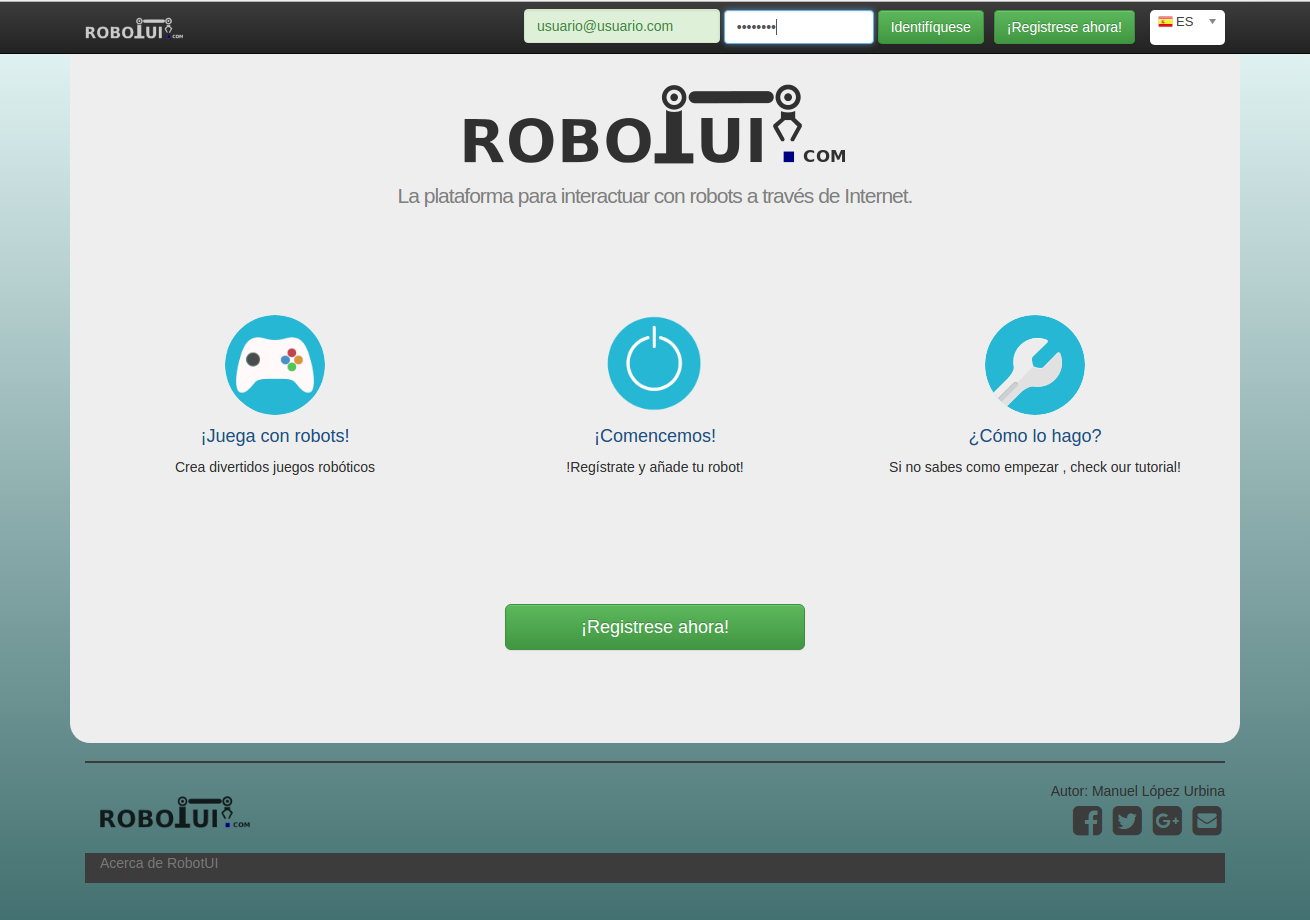
\includegraphics[scale=0.3]{imagenes/manual-usuario/pagina-principal.png}
  \end{center}
  \label{fig:logo}
 \caption{Página principal de de RobotUI.}
\end{figure}


El elemento hardware de este proyecto se compone de un vehículo controlado vía WiFi el cual responde a una serie de señales \emph{comandos} a los que responde realizando determinadas acciones.
La interfaz web se configurará de tal manera que permita el control del susodicho vehículo.\\

\begin{figure}[H]
  \begin{center}
    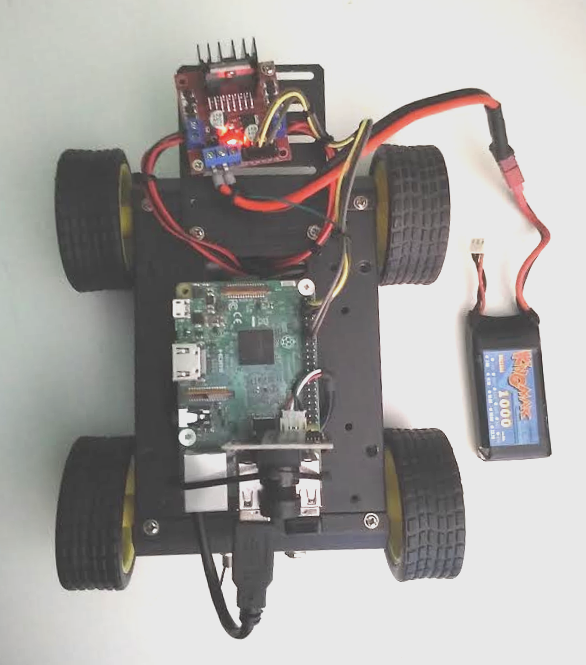
\includegraphics[scale=0.3]{imagenes/robot.jpg}
  \end{center}
  \label{fig:logo}
 \caption{Imagen del vehículo de pruebas desarrollado. \protect\footnotemark.}
\end{figure}

\footnotetext{Vehículo desarrollado para probar el funcionamiento de RobotUI. Su desarrollo y características quedan descritas en el capítulo \ref{chap:robot}.}


\section{Objetivos}
\label{sec:objetivos}

Como hemos visto, se requiere de multitud de conocimientos a la hora de afrontar un proyecto robótico con ciertas garantías. Este proyecto trata, al menos, de reducir, o facilitar, el área relacionada con
la informática, más concretamente con la programación. En la que multitud de personas ven en la programación un impedimento a la hora de comenzar a desarrollar sus ideas.
Por otro lado, existe la imperiosa necesidad de que la comunidad quiera mostrar sus creaciones al resto del mundo, compartir experiencias, problemas opiniones, etc, de una forma directa y no
mediante la grabación de vídeos del funcionamiento de los proyectos robóticos en cuestión, ya que no disponen de una herramienta adecuada para ello. En definitiva, existe la necesidad de que otros
usuarios puedan participar de manera más activa, ya sea visualizando el control por su creador o permitir que otros usuarios tomen el control de esos proyectos en tiempo real.
Por tanto este proyecto busca facilitar la árdua labor de programación de los proyectos robóticos junto con la posibilidad de compartir las creaciones realizadas con otros usuarios.\\

El sistema a desarrollar, por tanto, dispondrá de dos modos de funcionamiento, el primero de ellos proporciona las herramientas para la configuración de una interfaz a gusto del usuario, en la cual, 
una vez configurada, el usuario podrá controlar a su antojo el dispositivo. En el segundo modo de funcionamiento, la aplicación permitirá que otros usuarios puedan visitar la interfaz anteriormente 
configurada y actuar como espectadores en el control del robot por el usuario propietario del mismo. En definitiva, se proporcionará un sistema de control y difusión en uno solo.\\

\section{Acerca de este documento}

El documento se ha sido elaborado en un lenguaje claro y sencillo para permitir que un estudiante universitario de Ingeniería Informática pueda comprender los contenidos sin apenas dificultad añadida.\\

Este documento se organiza en los siguientes capítulos:\\

\begin{itemize}

\item En el capítulo \ref{chap:introducción}, Introducción, se comentan las razones que han motivado la creación de este proyecto, así como el propósito del mismo.

\item En el capítulo \ref{chap:conceptos-básicos}, Conceptos básicos, se incluyen definiciones de aquellos conceptos considerados de interés para la correcta comprensión del contenido de la presente memoria.

\item En el capítulo \ref{chap:herramientas}, Estado del arte y herramientas utilizadas, se realiza una descripción de las diferentes elementos hardware y software empleados durante el desarrollo del proyecto y necesarios para la utilización del mismo. Así como una breve descripción del conocimiento acumulado y tecnologías existentes hasta la fecha.

\item En el capítulo \ref{chap:requisitos}, Especificación y análisis de requisitos, se realiza una descripción de las diferentes elementos hardware y software empleados durante el desarrollo del proyecto y necesarios para la utilización del mismo. Así como una breve descripción del conocimiento acumulado y tecnologías existentes hasta la fecha.

\item En el capítulo \ref{chap:planificación}, Organización temporal, se recoge todo lo que concierne a la distribución y duración de cada una de las tareas llevadas a cabo durante el desarrollo del proyecto que el presente documento describe.

\item En el capítulo \ref{chap:dispositivos-hardware}, Configuración y montaje de los dispositivos hardware, se explica el proceso seguido para la correcta integración de los dispositivos hardware empleados describiendo la interconexión entre ellos así como su configuración. 

\item En el capítulo \ref{chap:desarrollo-software}, Desarrollo software, se realiza un análisis sobre la metodología empleada para el desarrollo software, describiendo los modelos de ciclo de vida utilizados, la descripción de los requisitos funcionales junto con el diagrama de casos de uso.

\item En el capítulo \ref{chap:reconocimiento}, Software de reconocimiento, se hace una descripción explicando los diferentes aspectos y elementos de cada uno de los prototipos desarrollados junto con los problemas encontrados y soluciones adoptadas.

\item En el capítulo \ref{chap:software-de-control}, Software de control, se describe cómo se ha llevado a cabo la comunicación ordenador-vehículo a nivel software.

\item En el capítulo \ref{chap:interfaz-gráfica}, Interfaz gráfica, se recogen aquellos aspectos técnicos de interés referentes a la elaboración de la interfaz gráfica.

\item En el capítulo \ref{chap:manual-usuario}, Guía de usuario, se describen los diferentes aspectos necesarios para la correcta utilización del conjunto software y hardware de los que se compone el presente proyecto.

\item En el capítulo \ref{chap:conclusiones}, Conclusiones, se hace mención de las conclusiones obtenidas tras la realización del proyecto además de las posibles mejoras aplicables.

\item En el capítulo Anexos \ref{chap:anexos}, aparecen los manuales de instalación del software que ha sido necesario para la realización del proyecto.

\end{itemize}


% Este archivo es parte de la memoria del proyecto fin de carrera
% de Manuel López Urbina. Protegida bajo la licencia GFDL.
% Para más información, la licencia completa viene incluida en el
% fichero fdl-1.3.tex

% Copyright (C) 2017 Manuel López Urbina

\chapter{Conceptos básicos}
\label{chap:conceptos-básicos}


En el presente capítulo se recogen aquellos conceptos, definiciones y protocolos que resultan de especial interés y que ayudarán a la comprensión de los diferentes puntos tratados en el resto de 
la memoria sin profundizar demasiado en detalles técnicos.

Todos estos conceptos se encuentran estrechamente ligados con tecnologías de la comunicación y transmisión de información, más concretamente en el ámbito de la programación web.

\section{Transmisión y comunicación}
\label{sec:transmisión}

Se denomina \emph{transmisión} como el proceso de transporte de una señal de un lugar a otro y \emph{comunicación} como el intercambio entre dos entes mediante una transmisión, los cuales son capaces de
interpretar la información circundante entre ellos y en el cual existen un conjunto de reglas definidas, los protocolos\footnote{Protocolo: reglamento o una serie de instrucciones que se fijan por tradición o por convenio. },
que rigen el proceso.


\section{Socket}
\label{sec:def-socket}

\emph{Socket} designa un concepto abstracto mediante el cual dos programas, generalmente situados en computadoras distintas, pueden intercambiar cualquier flujo de datos de manera fiable y ordenada.\\

El término \emph{socket} es también usado como el nombre de una interfaz de programación de aplicaciones (API) para la familia de protocolos de red TCP/IP \footnote{ TCP/IP es un conjunto de protocolos que
permiten la comunicación entre los ordenadores pertenecientes a una red. La sigla TCP/IP significa Protocolo de control de transmisión/Protocolo de Internet. Proviene de los nombres de dos protocolos 
importantes incluidos en el conjunto TCP/IP, es decir, del protocolo TCP y del protocolo IP. }, provista usualmente por el sistema operativo.\\

Los sockets constituyen el mecanismo para la entrega de paquetes de datos provenientes de la tarjeta de red a los procesos o hilos apropiados. Un socket queda definido por un par de direcciones IP local
y remota, un protocolo de transporte y un par de números de puerto local y remoto.\\

Cuando se habla de dirección y puerto local/remoto, se sobreentiende que nos referimos a dos procesos (cliente/servidor o nodo/nodo) ya que ambas direcciones IP y puerto pueden coincidir para el intercambio de información entre procesos dentro de una misma máquina
y; además, la comunicación puede ser perfectamente bidireccional, asumiendo que el par que la inicia es el cliente y su contrapartida un servidor pero pudiendo ejercer de forma ambivalente ambas partes.\\


\begin{figure}[H]
  \begin{center}
    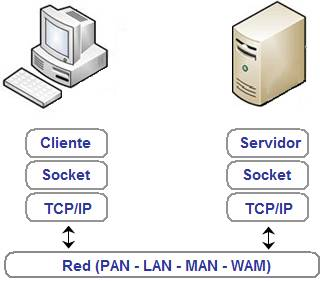
\includegraphics[scale=0.8]{imagenes/comunicaciones/socket.jpg}
  \end{center}
  \caption{ Representación de los sockets como una interfaz de la capa de transporte del protocolo TCP/IP.}
  \label{diagram:socket}
\end{figure}


\section{WebSocket}
\label{sec:def-websocket}

Comprendido previamente el concepto de \emph{socket} descrito en el punto \ref{sec:def-socket}, definimos  \emph{websocket} como una tecnología que proporciona un canal de comunicación bidireccional y full-duplex 
\footnote{Full Duplex: definido como la capacidad de transmisión y recepción en ambas direcciones al mismo tiempo. } utilizada por cualquier aplicación cliente/servidor.\\


La API de WebSocket está siendo normalizada por el W3C, mientras que el protocolo WebSocket ya fue normalizado por la IETF\footnote{Internet Engineering Task Force (IETF) (en español, Grupo de Trabajo de Ingeniería de Internet)
es una organización internacional abierta de normalización, que tiene como objetivos el contribuir a la ingeniería de Internet, actuando en diversas áreas, como transporte, encaminamiento, seguridad.
Se creó en los Estados Unidos, en 1986. Es mundialmente conocido porque se trata de la entidad que regula las propuestas y los estándares de Internet, conocidos como RFC.} como el RFC 6455.\\

Debido a que las conexiones TCP comunes sobre puertos diferentes al 80 son habitualmente bloqueadas por los administradores de redes, el uso de esta tecnología proporcionaría una solución
a este tipo de limitaciones proveyendo una funcionalidad similar a la apertura de varias conexiones en distintos puertos, pero multiplexando diferentes servicios WebSocket sobre un único
puerto TCP a costa de una pequeña sobrecarga del protocolo.


\section{Streaming}
\label{sec:def-streaming}


La retransmisión (en inglés streaming, también denominado transmisión) es la distribución digital de contenido multimedia a través de una red de computadoras, 
de manera que el usuario utiliza el producto a la vez que se es descargado. La palabra retransmisión se refiere a una corriente continua que fluye sin interrupción, habitualmente audio o vídeo, aplicándose la difusión 
de vídeo en el presente proyecto. \\

Este tipo de tecnología funciona mediante un búfer de datos que va almacenando el flujo de descarga en la estación del usuario para inmediatamente mostrarle el material descargado. Esto se contrapone al mecanismo de
descarga de archivos, que requiere que el usuario descargue los archivos por completo para poder acceder al contenido.\\

La retransmisión requiere de una conexión por lo menos de igual ancho de banda que la tasa de transmisión del servicio. La retransmisión de vídeo por Internet se popularizó a fines de la década de 2000, 
cuando la contratación del suficiente ancho de banda para utilizar estos servicios en el hogar se hizo lo suficientemente barato.



\section{Framework}
\label{sec:def-Framework}

Un framework, también denominado entorno de trabajo o marco de trabajo, es un conjunto estandarizado de conceptos, prácticas y criterios para enfocar un tipo de problemática particular que sirve como
referencia, para enfrentar y resolver nuevos problemas de índole similar.\\

Aplicado a informática, concretamente al desarrollo de software, un entorno de trabajo o framework es una estructura conceptual y tecnológica de asistencia definida, normalmente, con artefactos o 
módulos concretos de software, que puede servir de base para la organización y desarrollo software. Típicamente, puede incluir soporte de programas, bibliotecas, y un lenguaje interpretado, entre 
otras herramientas, para así ayudar a desarrollar y unir los diferentes componentes de un proyecto.\\

En  general,  con  el  término  framework, nos estamos refiriendo a una estructura software compuesta de componentes personalizables e intercambiables para el
desarrollo de una aplicación. En otras palabras, un framework se puede considerar como una aplicación genérica incompleta y configurable a la que podemos añadirle las últimas 
piezas para construir una aplicación concreta.\\

Los objetivos principales que persigue un framework son:

\begin{itemize}
 \item Acelerar el proceso de desarrollo
 \item Reutilización de código.
 \item Promover buenas prácticas de desarrollo como el uso de patrones.
\end{itemize}




% Este archivo es parte de la memoria del proyecto fin de carrera
% de Manuel López Urbina. Protegida bajo la licencia GFDL.
% Para más información, la licencia completa viene incluida en el
% fichero fdl-1.3.tex

% Copyright (C) 2017 Manuel López Urbina

\chapter[Herramientas utilizadas]{Estado del arte y tecnologías utilizadas}
\chaptermark{Arte y tecnologías}
\label{chap:herramientas}


\section{Estado del arte}

En la actualidad podemos observar cómo la robótica cada vez se encuentra más presente en nuestras vidas cotidianas tanto como para facilitarnos ciertas tareas como para entretenimiento. Si realizamos 
cualquier búsqueda en internet podemos encontrar multitud de proyectos robóticos en la red. Existen excelentes portales como \url{http://blog.bricogeek.com/} por nombrar alguno de ellos, donde se
publican multitud de proyectos novedosos y originales donde sus autores describen su desarrollo y por regla general lo acompañan de un vídeo donde se demuestra su funcionamiento.\\

Existen también comunidades que organizan competiciones de drones y/o robots, comunidades educativas asociadas a alguna tecnología concreta como pueden ser Arduino o Raspberry Pi, etcétera, donde nuevamente todas las 
descripciones de los diferentes proyectos se realizan con la documentación oportuna y en la mayoría de los casos acompañadas de un vídeo demostrativo con la inexistencia de interacción directa por parte 
del usuario.\\


Dado lo anterior, considero que hay un campo sin cubrir y que resultaría interesante abarcar este espacio con una aplicación con las características de RobotUI, ya que no existe
ninguna plataforma que permita esta interacción usuario-máquina o usuarios-máquina en tiempo real y que sea configurable para cualquier dispositivo que se encuentre conectado a la red.\\



\section{Tecnologías software utilizadas}
\sectionmark{Tecnologías software}


A continuación se detallan las diferentes tecnologías/bibliotecas/lenguajes que se han empleado para la elaboración del proyecto y por qué se han escogido por encima de otras posibles soluciones.


\subsection{\LaTeX}

Web: \url{https://www.latex-project.org/}\\

\LaTeX es un lenguaje de marcado que sirve para la redacción de documentos científicos o técnicos. Con esta herramienta o lenguaje se ha desarrollado la memoria actual del proyecto de final de carrera.



\subsection{WebStorm}

\hspace*{2.25in}{
\includegraphics[scale=0.25]{imagenes/webstorm-logo.png}}

Web: \url{https://www.jetbrains.com/webstorm/}\\

WebStorm es un IDE de JavaScript ligero pero potente, perfectamente equipado para el desarrollo del lado del cliente y el desarrollo del servidor con Node.js. Permite la integración con frameworks de desarollo como Sails js. Para el desarrollo de la aplicación se optó por este IDE. \\

\subsection{Github}


\hspace*{2.25in}{
\includegraphics[scale=0.25]{imagenes/github-logo.png}}

Web: \url{https://about.github.com/}\\
Repositorio: \url{https://github.com/lopi87/SAILS-RobotUI}\\


GitHub es una forja (plataforma de desarrollo colaborativo) para alojar proyectos utilizando el sistema de control de versiones Git. Utiliza el framework Ruby on Rails por GitHub, Inc. (anteriormente conocida como Logical Awesome). Desde enero de 2010, GitHub opera bajo el nombre de GitHub, Inc. El código se almacena de forma pública, aunque también se puede hacer de forma privada, creando una cuenta de pago.


\subsection{Git}

\hspace*{2.1in}{
\includegraphics[scale=0.5]{imagenes/git-logo.png}}

Web: \url{https://git-scm.com/}\\

Git es un sistema open-source de control de versiones diseñado para manejar íntegramente las fases de desarrollo de proyectos, simples y complejos, con velocidad y eficiencia.\\

\subsection{DigitalOcean}

\begin{center}
\includegraphics[scale=0.35]{imagenes/docean-logo.png}\end{center}

Web: \url{https://www.digitalocean.com/}\\

Servidor web para alojar proyectos en la nube. La ventaja de este servicio de VPS \footnote{ VPS: Servidor Virtual Privado, del inglés Virtual Private Server, es un método de particionar un servidor
físico en varios servidores de tal forma que todo funcione como si se estuviese ejecutando en una única máquina. Cada servidor virtual es capaz de funcionar bajo su propio sistema operativo y
además cada servidor puede ser reiniciado de forma independiente.} es que te permite desplegar máquinas de cualquier tipo (siempre que sean software libre) de una manera muy fácil y rápida. 
Además tiene un punto fuerte y es que la información se almacena en discos SSD, con lo que el procesamiento se ve muy mejorado a la hora de computar (en este caso trabajo con websockets y 
transmisión de datos).\\

\begin{figure}[H]
\begin{center}
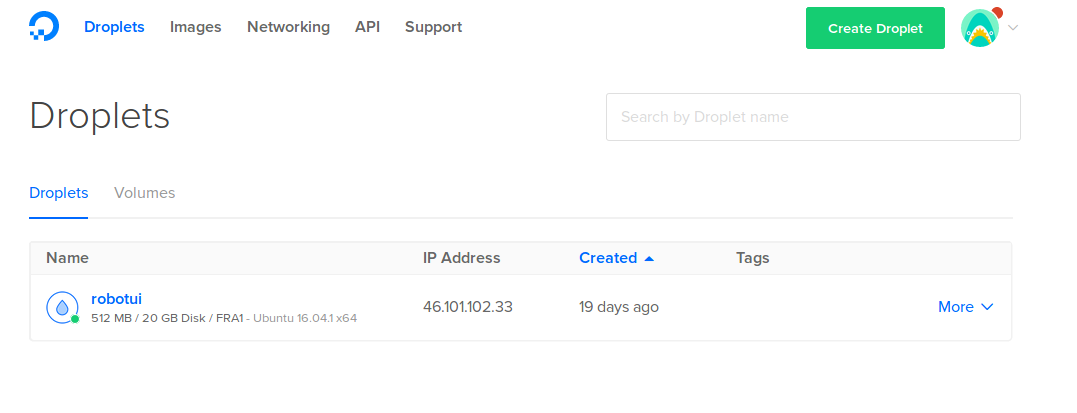
\includegraphics[scale=0.45]{imagenes/droplets.png}
\caption{Droplet desplegado en DigitalOcean}
\end{center}
\end{figure}


\subsection{Node js}

\begin{center}

\includegraphics[scale=0.3]{imagenes/nodejs-logo.png}
\end{center}

Web: \url{https://nodejs.org/es/}\\

Node.js es un entorno de ejecución para JavaScript construido con el motor de JavaScript V8 de Chrome. Node.js usa un modelo de operaciones E/S sin bloqueo y orientado a eventos, que lo hace liviano y eficiente. Incorpora un sistema de gestión de paquetes llamado, npm, es el ecosistema mas grande de librerías de código abierto en el mundo.\\

Node.js tiene una arquitectura basada en eventos capaz de E/S asíncronos. Estas opciones de diseño apuntan a optimizar el rendimiento y la escalabilidad en aplicaciones Web con muchas operaciones de entrada/salida, así como para aplicaciones Web en tiempo real (por ejemplo, programas de comunicación en tiempo real y juegos de navegador), lo que lo hacen ideal para este proyecto.\\


\subsection{Sails js}

\begin{center}

\includegraphics[scale=0.5]{imagenes/sailsjs-logo.png}
\end{center}

Web: \url{http://sailsjs.com/}\\

Sails.js es un framework web que facilita la creación de aplicaciones Node.js de nivel empresarial. Está diseñado para asemejarse a la arquitectura MVC de otros frameworks como Ruby on Rails, pero con soporte para el estilo de desarrollo de aplicaciones web más moderno y orientado a datos.\\

Utiliza Express para funciones como la gestión de peticiones HTTP y websockets. Su integración con el sistema de websockets lo hacen especialmente bueno para construir características en tiempo real. Por estas razones se ha considerado como el framework más adecuado hasta la fecha para la elaboración de este proyecto.


\subsection{Npm}

\begin{center}

\includegraphics[scale=0.4]{imagenes/npm-logo.png}
\end{center}

Web: \url{https://www.npmjs.com/}\\

npm es el gestor de paquetes por defecto para Node.js, un entorno de ejecución para JavaScript. Utilizado para la descarga de las librerías incorporadas al proyecto.


\subsection{SocketIO}

\begin{center}

\includegraphics[scale=0.3]{imagenes/socketio-logo.png}
\end{center}

Web: \url{https://socket.io/}\\

Socket.IO es una biblioteca de JavaScript para aplicaciones web en tiempo real. Permite la comunicación bidireccional en tiempo real entre clientes web y servidores. Consta de dos partes: una biblioteca del lado del cliente
que se ejecuta en el navegador y una biblioteca del lado del servidor para Node.js. Ambos componentes tienen una API casi idéntica. Al igual que Node.js, es impulsado por eventos.

Socket.IO puede usarse simplemente como un wrapper para WebSocket aunque proporciona muchas más funciones, incluyendo la transmisión a múltiples sockets, almacenamiento de datos asociados a cada cliente y E/S asíncronas.


\subsection{ FFmpeg }


\begin{center}

\includegraphics[scale=0.75]{imagenes/Ffmpeg-logo.jpg}
\end{center}

Web: \url{https://ffmpeg.org/}\\

FFmpeg es una colección bibliotecas software libre que permiten grabar, convertir (transcodificar) y hacer streaming de audio y vídeo. Incluye libavcodec, una biblioteca de códecs. FFmpeg está desarrollado en GNU/Linux, pero puede ser compilado
en la mayoría de los sistemas operativos, incluyendo Windows.

FFmpeg es un programa bastante sencillo y de fácil utilización, orientado tanto a personas con conocimientos avanzados como usuarios inexpertos. 

El proyecto FFmpeg está compuesto por:

\begin{itemize}
 \item ffmpeg: es una herramienta de línea de comandos para convertir audio o video de un formato a otro. También puede capturar y codificar en tiempo real desde DirectShow, una tarjeta de televisión u otro dispositivo compatible.
 \item ffserver: es un servidor de streaming multimedia de emisiones en directo que soporta HTTP (la compatibilidad con RTSP está en desarrollo). Todavía no está en fase estable, y de momento no está disponible para Windows.
 \item ffplay: es un reproductor multimedia basado en SDL y las bibliotecas FFmpeg.
 \item libavcodec: es una biblioteca que contiene todos los códecs de FFmpeg. Muchos de ellos fueron desarrollados desde cero para asegurar una mayor eficiencia y un código altamente reutilizable.
 \item libavformat: es una biblioteca que contiene los multiplexadores/demultiplexadores para los archivos contenedores multimedia.
 \item libavutil: es una biblioteca de apoyo que contiene todas las rutinas comunes en las diferentes partes de FFmpeg.
 \item libpostproc: es una biblioteca de funciones de postproceso de vídeo.
 \item libswscale: es la biblioteca de escalado de vídeo.
\end{itemize}

Para el desarrollo de RobotUI, concretamente para la transmisión de vídeo desde el robot de pruebas desarrollado hacia el cliente, el módulo utilizado ha sido el de la herramienta de línea de comandos.


\subsection{Bootstrap}


\begin{center}

\includegraphics[scale=0.3]{imagenes/bootstrap-logo.jpg}
\end{center}

Web: \url{http://getbootstrap.com/}\\

Bootstrap es un framework o conjunto de herramientas de código abierto para diseño de sitios y aplicaciones web. Contiene plantillas de diseño con tipografía, formularios, botones, cuadros, menús de navegación y otros elementos de diseño basado en HTML y CSS, así como, extensiones de JavaScript opcionales adicionales. Se ha utilizado en el presente proyecto para la maquetación de la aplicación.

\subsection{JQuery}


\begin{center}

\includegraphics[scale=0.7]{imagenes/jquery-logo.png}
\end{center}

Web: \url{https://jquery.com/}\\

JQuery es una biblioteca de JavaScript rápida, pequeña y característica. Hace que las cosas como manipulación del código HTML, manejo de eventos, animación, y permite la realización de 
peticiones Ajax de manera mucho más simple gracias a API de fácil manejo, la cual funciona a través de una multitud de navegadores. Gracias a su combinación de versatilidad y extensibilidad jQuery
ha cambiado la forma en que millones de personas desarrollan con JavaScript.\\


\subsection{Mongo DB}

\begin{center}

\includegraphics[scale=0.5]{imagenes/mongodb-logo.png}
\end{center}


Web: \url{https://www.mongodb.com/es}\\

MongoDB ( cuyo nombre proviene de la palabra en inglés “humongous” que significa enorme ) es un sistema de base de datos NoSQL orientado a documentos, desarrollado bajo el concepto de código abierto.\\

La principal particularidad de las bases de datos NoSQL es que en lugar de guardar los datos en tablas como se hace en las base de datos relacionales, guarda estructuras de datos en documentos 
similares a JSON con un esquema dinámico (MongoDB utiliza una especificación llamada BSON), haciendo que la integración de los datos en ciertas aplicaciones sea más fácil y rápida.\\

\subsection{Pm2}

\begin{center}

\includegraphics[scale=0.4]{imagenes/pm2-logo.png}
\end{center}

Web: \url{http://pm2.keymetrics.io/}\\


PM2 es un gestor de procesos de producción para aplicaciones Node.js con un balanceador de carga incorporado. Permite mantener las aplicaciones en ejecución, recargarlas sin tiempo de inactividad
y facilitar las tareas comunes del administrador de sistemas.


\subsection{ Robomongo }

\begin{center}

\includegraphics[scale=0.5]{imagenes/robomongo-logo.png}
\end{center}

Web: \url{https://robomongo.org/}\\


Robomongo es una herramienta de gestión MongoDB de código abierto multi-plataforma basada en shell que incorpora el mismo motor de JavaScript que potencia el shell mongo de MongoDB.
Una de sus particularidades es que Robomongo no sólo analiza la semántica del código, sino que también lo ejecuta en una máquina virtual JavaScript interna, lo que permite dotar a la 
herramienta de un autocompletado en tiempo de ejecución imposible de obtener de forma estática. Esta herramienta ha sido de especial ayuda para la gestión de la base de datos del proyecto.\\


\section{Tecnologías hardware y materiales utilizados}
\sectionmark{Tecnologías hardware}
\label{sec:tecnologias-hardware}


A continuación se detallan las diferentes tecnologías hardware que se han
empleado para la elaboración del vehículo robótico con la finalidad de servir de prototipo durante el desarrollo de la aplicación y a modo demostrativo de la misma. En los sucesivos puntos
se describen las características de cada una de ellas junto con el motivo de su elección.


\subsection{Raspberry Pi Model B}
\label{sec:raspberry}



\begin{center}

\includegraphics[scale=0.3]{imagenes/RaspberryPi-logo.png}
\end{center}

Web: \url{https://www.raspberrypi.org}\\

Raspberry Pi es un ordenador de tamaño reducido y de bajo coste desarrollado en Reino Unido por la Fundación Raspberry Pi, con el objetivo de estimular la enseñanza de ciencias de la computación
en las escuelas. Es ampliamente utilizado y de uso muy extendido por lo que ha sido el principal motivo de su elección, además de su bajo cote y versatilidad.\\

La Raspberry Pi 3 es la tercera generación de Raspberry Pi. Sus especificaciones son las siguientes:

\begin{itemize}
 \item Una CPU ARMv8 quad-core de 64 bits de 64 bits y 1.2 GHz
 \item LAN inalámbrica 802.11n
 \item Bluetooth 4.1
 \item Bluetooth baja energía (BLE)
 \item 1 GB de RAM
 \item 4 puertos USB
 \item 40 conexiones GPIO
 \item Puerto HDMI
 \item Puerto Ethernet
 \item Conector de audio combinado de 3,5 mm y vídeo compuesto
 \item Interfaz de la cámara (CSI)
 \item Interfaz de pantalla (DSI)
 \item Ranura para tarjeta Micro SD
 \item VideoCore IV núcleo de gráficos 3D 
\end{itemize}


\begin{figure}[H]
  \begin{center}
    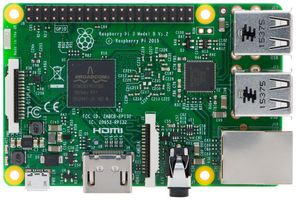
\includegraphics[scale=0.5]{imagenes/raspberry-pi.jpg}\\
    \caption{Imagen de una Raspberry Pi 3 Model B}
  \end{center}
\end{figure}


\subsection{Controladora de motores L298N}


El módulo controlador de motores L298N H-bridge nos permite controlar la velocidad y la dirección de dos motores de corriente continua o un motor paso a paso de una forma muy sencilla,
gracias a los 2 los dos H-bridge que dispone.\\

básicamente un puente-H o H-bridge es un componente formado por 4 transistores que nos permite invertir el sentido de la corriente, y de esta forma podemos 
invertir el sentido de giro del motor.\\

El rango de tensiones en el que trabaja este módulo va desde 3V hasta 35V, y una intensidad de hasta 2A. A la hora de alimentarlo hay que tener en cuenta que la 
electrónica del módulo consume unos 3V, así que los motores reciben 3V menos que la tensión con la que alimentemos el módulo.\\

Además el L298N incluye un regulador de tensión que nos permite obtener del módulo una tensión de 5V, perfecta para alimentar nuestro Arduino. Eso sí, este regulador sólo 
funciona si alimentamos el módulo con una tensión máxima de 12V.\\

Es un módulo que se utiliza mucho en proyectos de robótica, por su facilidad de uso y su reducido precio, lo cual ha servido para que sea seleccionado para el presente proyecto.

\begin{figure}[H]
  \begin{center}
    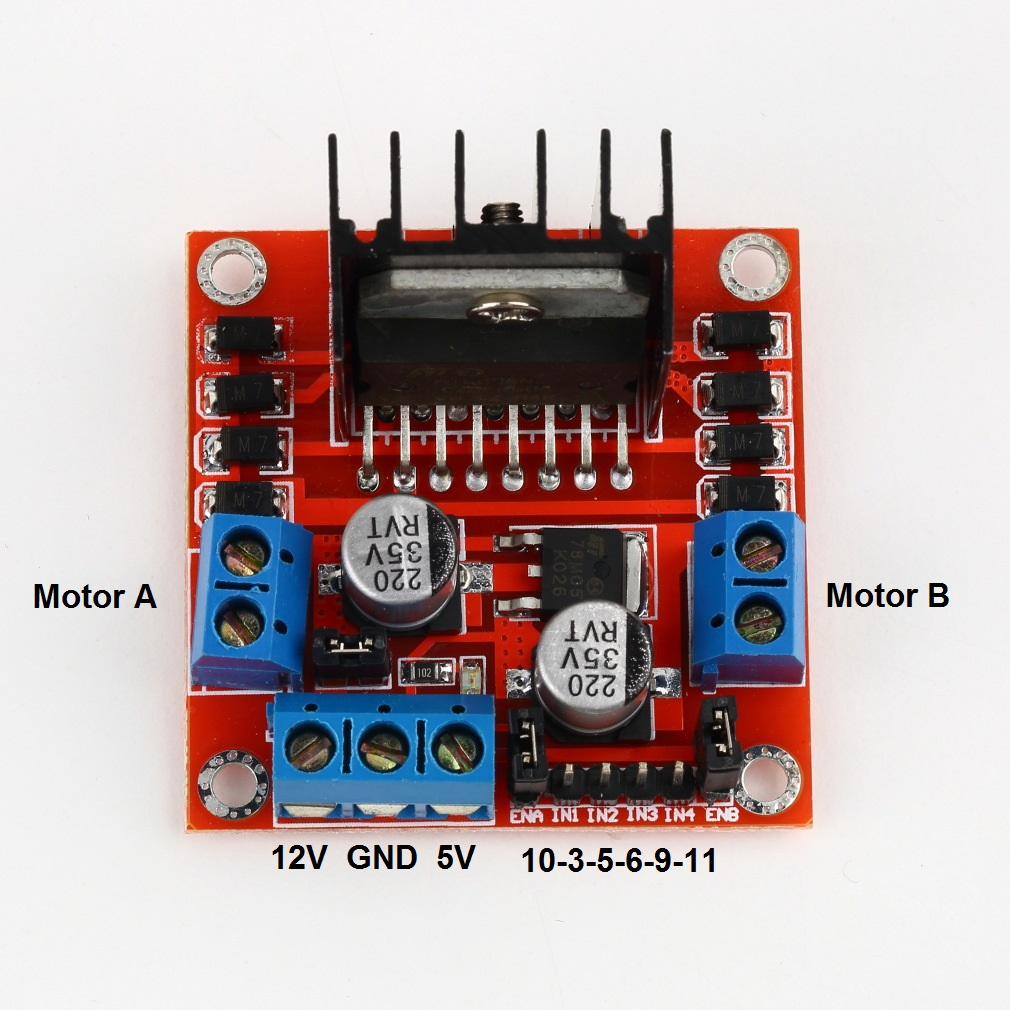
\includegraphics[scale=0.8]{imagenes/l298n.jpg}\\
    \caption{Imagen de la controladora de motores L298n utilizada.}
  \end{center}
\end{figure}



\subsection{ Batería LiPo }

Para alimentar los motores y su controladora se ha empleado una batería LiPo de 1000mAh a 3,7V. Las batería de polímero de iones de litio, son pilas recargables (células de secundaria), compuestas generalmente de varias células secundarias idénticas en paralelo para aumentar la capacidad 
de la corriente de descarga. Siendo ideales para este tipo de usos.

\begin{figure}[H]
  \begin{center}
    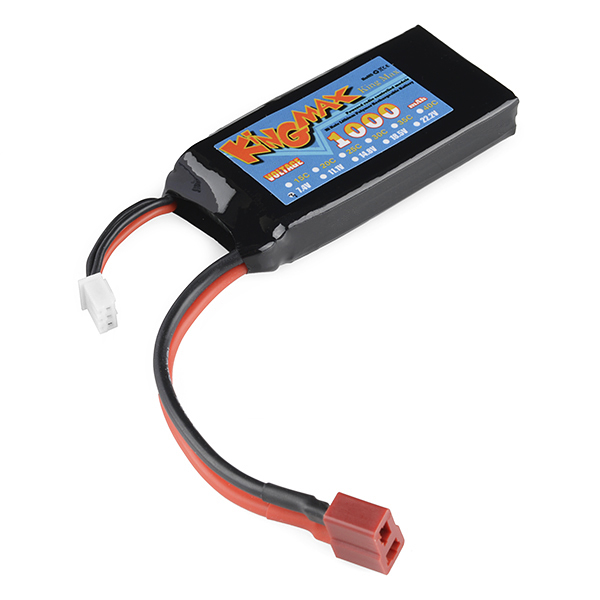
\includegraphics[scale=0.3]{imagenes/robot/bateria-lipo.jpg}\\
    \caption{Imagen de la batería LiPo utilizada.}
  \end{center}
\end{figure}


\subsection{ Tarjeta de expansión con batería de Litio para Raspberry Pi }
\label{componente:bateria-expansion}

Para la alimentación de la placa se ha optado por un módulo de potencia diseñado especialmente para la Raspberry Pi 3 Model B, permitiendo que la placa maestra trabaje sin conexión hasta 9 horas
de forma ininterrumpida.\\

Por otra parte, esta placa dispone de 2 puertos USB adicionales: uno suministra energía para la Raspberry Pi y el otro para una posible pantalla LCD, resultando interesante para otros proyectos.\\

Sus características principales son las siguientes:

\begin{enumerate}
 \item Capacidad de la batería: 3800mAH
 \item Corriente de descarga máxima: 1.8A
 \item Tensión de salida sin carga: 5.1V ± 0.1V
 \item Corriente / voltaje de carga estándar: 1.0A / 5.0V
 \item Tensión de corte de la carga completa de la batería de iones de litio: 4.18V - 4.2V
\end{enumerate}


\begin{figure}[H]
  \begin{center}
    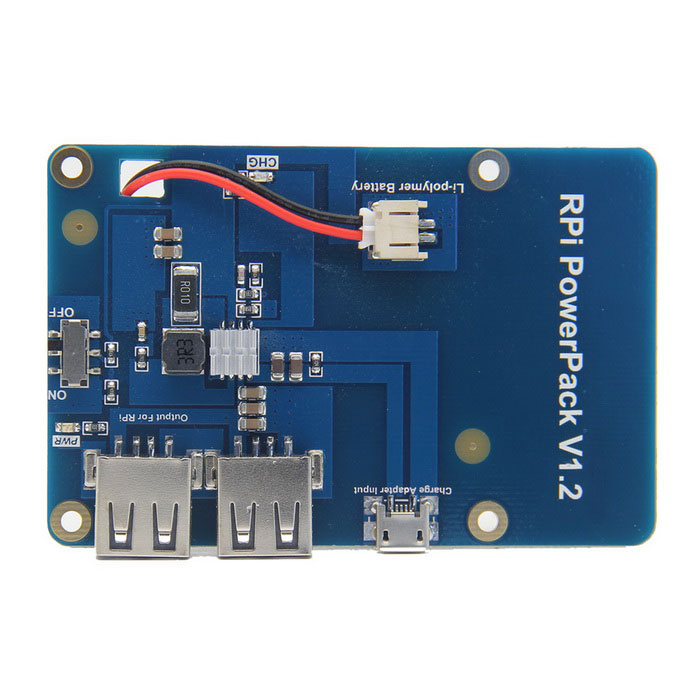
\includegraphics[scale=0.3]{imagenes/robot/modulo-alimentacion.jpg}\\
    \caption{Imagen de la tarjeta de expansión con batería de Litio utilizado.}
  \end{center}
\end{figure}

\subsection{ Cámara USB de alta definición }

Cámara USB para su conexión en la Raspberry para la emisión de imágenes. La cámara seleccionada dispone de las siguientes características:

\begin{itemize}
\item 2 megapíxeles de resolución.
\item Ángulo de visión de 170 grados.
\item Interfaz USB 2.0 de alta velocidad, refresco de 60 fps en resolución 1280X720, 30 fps en resolución 1920X1080
\item Tamaño reducido y perfil delgado ideal para aplicaciones embebidas.
\end{itemize}

\begin{figure}[H]
  \begin{center}
    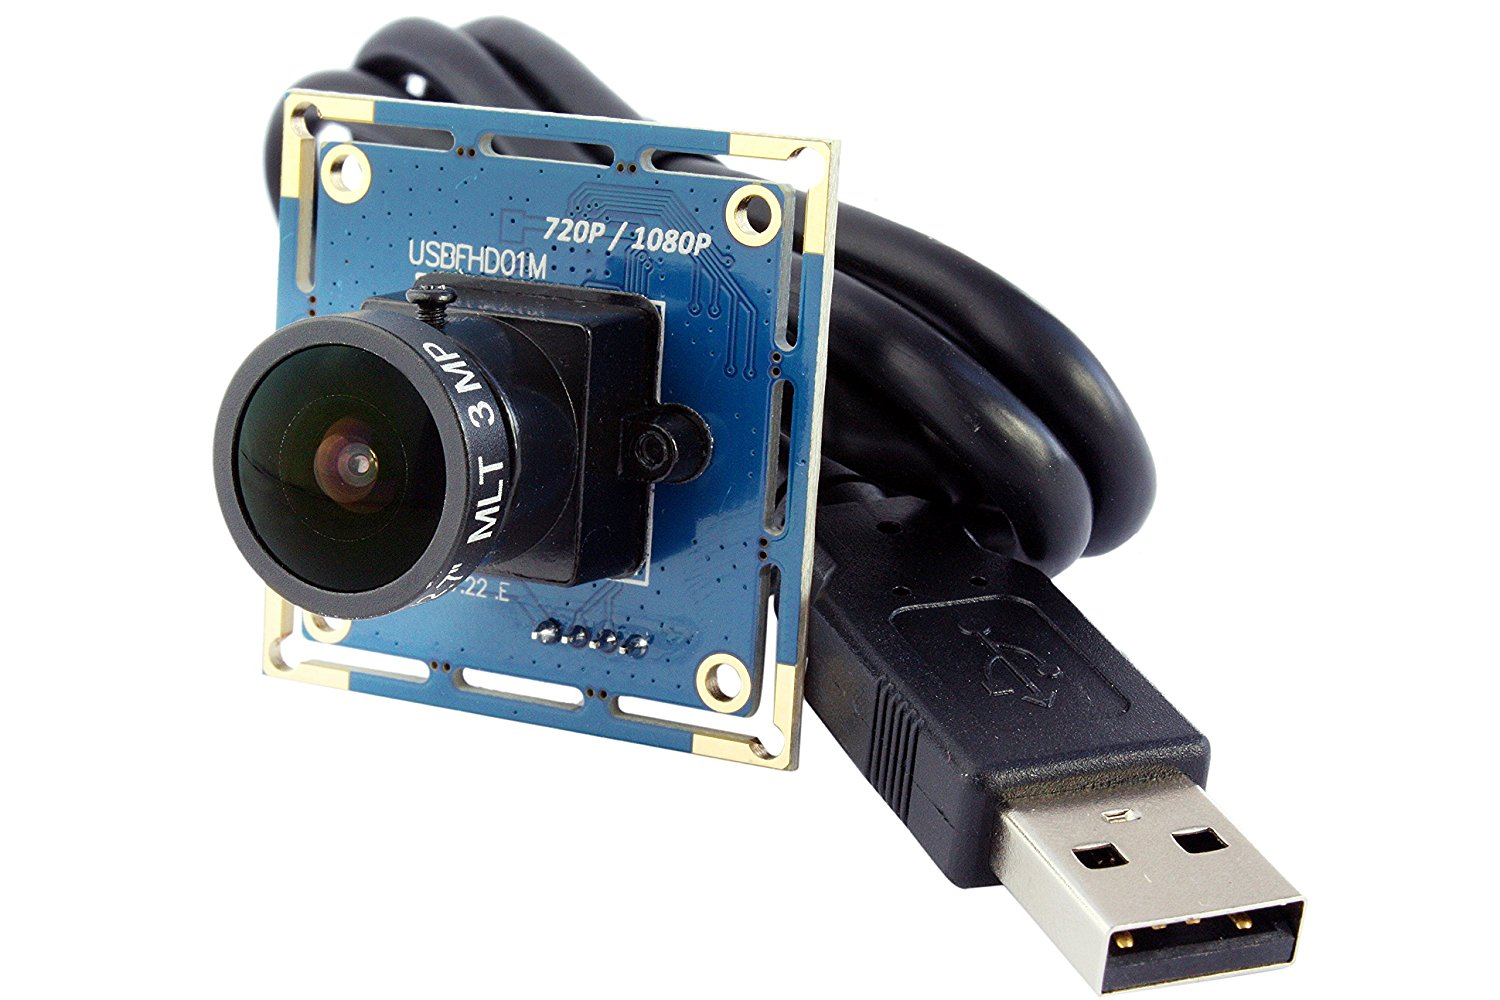
\includegraphics[scale=0.15]{imagenes/robot/camara-usb.jpg}\\
    \caption{Imagen de la cámara USB utilizada.}
  \end{center}
\end{figure}

Los motivos de su elección ha sido principalmente su facilidad de puesta en funcionamiento ya que al tratarse de una cámara USB. Tan sólo debemos conectarla para comenzar con su funcionamiento ya que es detectada 
por prácticamente todas las distribuciones Linux. 

\newpage

\chapter{Desarrollo software }
\chaptermark{desarrollo}
\label{chap:desarrollo-software}


\section{Metodología de desarrollo}

Este proyecto ha sido elaborado empleando una metodología de desarrollo basada en el modelo de desarrollo incremental para la parte software referente a todos los subsistemas web y una metodología de 
desarrollo en cascada para el desarrollo de la parte software referente al robot de pruebas.\\

El modelo de desarrollo incremental proporciona una serie de características que lo hacen idóneo para este proyecto. Dicho modelo se basa en la filosofía de construir 
e ir incrementando las funcionalidades del sistema mediante el desarrollo de los diferentes módulos. Esto permite ir aumentando gradualmente las capacidades del software. \\

Dicha metodología de desarrollo resulta especialmente útil en las siguientes situaciones:\\

\begin{itemize}
 \item Facilita el desarrollo permitiendo a cada miembro del equipo desarrollar un módulo particular. En el caso del presente proyecto me ha permitido desarrollar un módulo tras otro de una manera secuencial.
 \item Es similar al ciclo de vida en cascada aplicándose un ciclo en cada nueva funcionalidad del programa.
 \item A final de cada ciclo se entrega el software al cliente. En el caso que compete a este proyecto se mantenía una reunión con el director del proyecto para su aprobación.
\end{itemize}

Centrándonos nuevamente en el desarrollo del proyecto, los motivos que llevaron a cabo la elección de un modelo de desarrollo incremental viene dada por la necesidad de simplificar e ir
desarrollando de una forma gradual y modularizada debido a la extensión del proyecto. Más si cabe que el equipo de desarrollo solo consta de una persona.\\

Por otro lado, para el desarrollo del vehículo de pruebas y por su simplicidad, se ha optado por un desarrollo en cascada. El modelo de desarrollo en cascada resulta adecuado en situaciones
en las que:\\

\begin{itemize}
 \item Se dispone de unos requisitos claros y precisos.
 \item El sistema a desarrollar es de pequeña envergadura.
 \item Las tecnologías utilizadas son conocidas por los desarrolladores.
\end{itemize}

Siendo precisamente éstas las características del del proyecto del vehículo a desarrollar puesto que se trata de un desarrollo de pequeño tamaño y las herramientas empleadas ya me resultaban conocidas
tras la realización de otros trabajos previos.\\

Por tanto el proyecto queda distribuido en los siguientes subsistemas:\\

\begin{figure}[H]
  \begin{center}
    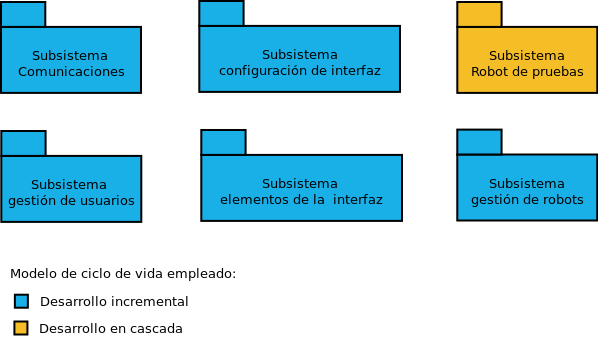
\includegraphics[scale=.6]{diagramas/subsistemas.png}
  \end{center}
  \caption{Subsistemas existentes en el proyecto junto con el modelo de ciclo de vida
utilizado para su desarrollo.}
  \label{website:pagina-principal}
\end{figure}


\section{Recolección de requisitos}

\subsection{Requisitos funcionales}

Para la elaboración de este proyecto se ha utilizado la metodología Métrica V3 así como el estándar ISO/IEC 12207. Métrica es una metodología de planificación, desarrollo y
mantenimiento de los sistemas de información desarrollada por el Ministerio de Administraciones Públicas del Gobierno de España. Tiene como objetivo proporcionar una guía para 
la sistematización de actividades del ciclo de vida de los proyectos software en el ámbito de las administraciones públicas.\\

Métrica V3 \cite{website:metrica} está basada en el modelo de procesos del ciclo de vida de desarrollo ISO/IEC 12207 (Information Technology - Software Life Cycle Processes) así como
en la norma ISO/IEC 15504 SPICE (Software Process Improvement And Assurance Standards Capability Determination).\\

En la página oficial de Métrica V3, sus desarrolladores indican que puede ser utilizada libremente con la única restricción de citar la fuente de su propiedad intelectual, 
la del Ministerio de Administraciones Públicas.\\

En esta etapa del modelado de requisitos se captura el propósito general del sistema:

\begin{itemize}
  \item Se analiza qué debe hacer el sistema.
  \item Se obtiene una versión contextualizada del sistema.
  \item Identifica y delimita el sistema.
  \item Se determinan las características, cualidades y restricciones que debe satisfacer el sistema.
\end{itemize}


Por tanto, Los requisitos funcionales que se han obtenido después del proceso de obtención de requisitos son:\\

\begin{itemize}
  \item Definir los pasos para dar de alta un dispositivo robótico en el sistema.
  \item Una vez configurado el dispositivo, configurar la interfaz de control con las acciones de control específicas.
  \item Realizar un sistema de monitorización y visualización para los usuarios y los dispositivos robóticos en tiempo real.
  \item Sistema de gestión de base de datos en donde se encuentren los datos de la aplicación recogidos.
  \item Disponer de un panel de administración donde visualizar la información de los usuarios conectados y dispositivos en uso en tiempo real. 
  \item Proporcionar un sistema de streaming de vídeo para la difusión de imágenes a los usuarios espectadores procedentes de los robots dispongan de cámara.
  \item Deberá ser una herramienta multiplataforma.  
\end{itemize}



\subsection{Requisitos no funcionales}

Los requisitos no funcionales son aquellos que describen cualidades o restricciones del sistema que no se relacionan de forma directa con el comportamiento funcional del mismo. A continuación se especifican los más importantes del sistema:
\begin{itemize}
\item No requiere un conocimiento específico del sistema una vez puesto en funcionamiento.
\item La aplicación tendrá manual de uso.
\item La base de datos estará implementada en un lenguaje objeto no relacional como MongoDB.
\item La aplicación estará realizada en el lenguaje de programación Python.
\item La interfaz debe reflejar claramente la distinción entre las distintas partes del sistema.
\item El sistema se desplegará sobre una versión GNU Linux Debian 8 Jessie.
\item El código fuente de la aplicación seguirá un estilo uniforme y normalizado para todos los módulos del mismo.
\end{itemize}


\section {Diagrama de casos de uso}

Un caso de uso es una descripción de los pasos o actividades que deberán realizarse para llevar a cabo algún proceso. Los objetivos de los casos de uso son los siguientes:

\begin{itemize}
\item Obtener los requisitos funcionales del sistema y expresarlos desde un punto de vista más cercano al usuario.
\item Proporcionar una guía de todo el proceso de desarrollo del sistema de información. Los casos de uso proporcionan, por tanto, un modo claro y preciso de comunicación entre lo que desea el cliente y el desarrollador proporcionando desde el punto de vista del cliente una visión de ``caja negra'' del sistema eliminando los detalles de su construcción o desarrollo. Para los desarrolladores es utilizado como punto de partida y el eje sobre el que se apoya todo el desarrollo del sistema en los procesos de análisis y diseño.
\end{itemize}

Los diagramas de caso de uso muestran una representación del comportamiento ofrecido por el sistema de información desde el punto de vista del usuario. El comportamiento
del sistema es representado como un conjunto de transacciones ejecutadas entre el sistema y los actores junto con la descripción sobre las de las relaciones de comunicación
existentes entre un actor y el sistema.\\

En la figura \ref{diagram:caso-uso} podemos observar los diagramas de casos de uso resultantes tras la recolección de requisitos:

\begin{figure}[H]
  \begin{center}
    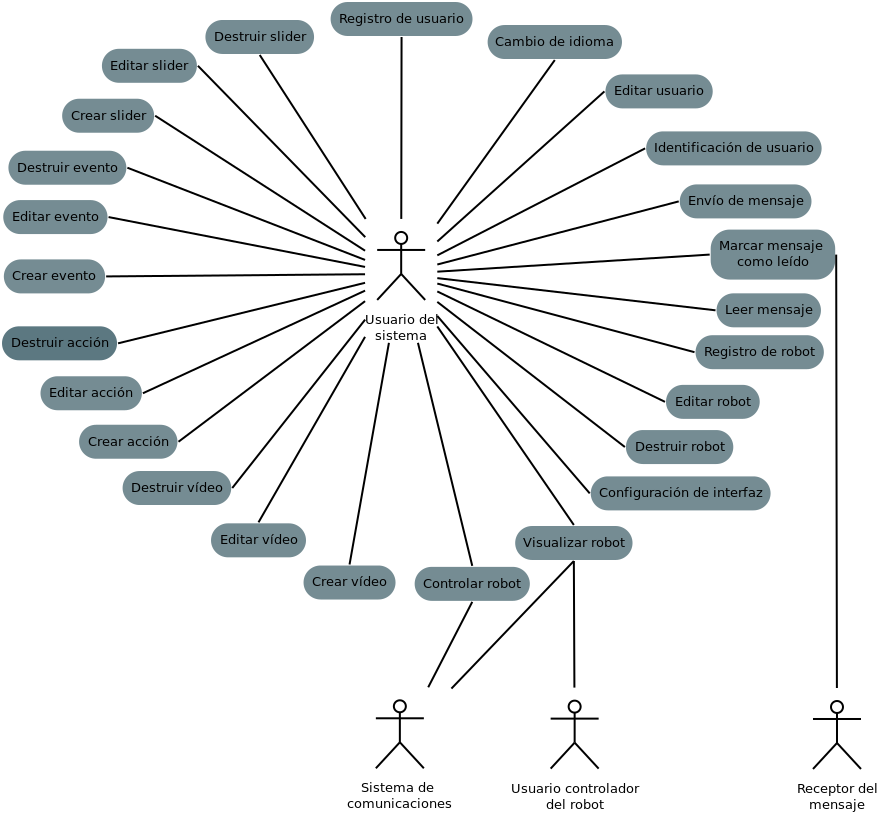
\includegraphics[scale=.5]{diagramas/casos-uso.png}
  \end{center}
  \caption{Diagrama de casos de uso para la interacción con la aplicación.}
  \label{diagram:caso-uso}
\end{figure}


\section{Descripción de los casos de uso}
\label{sec:especificaciones-caso-uso}

A continuación se proporciona la especificaciones de cada uno de los casos de uso de la figura \ref{diagram:caso-uso}:


\begin{table}[H]
  \begin{center}
    \begin{tabular}{|p{3.5cm}|p{10cm}|}
      \hline
      {\textbf{Caso de uso:}} & { Registro de usuario.} \\
      \hline
      {\textbf{Descripción:}} & { El sistema deberá actuar como describe en este caso de uso cuando el usuario solicita el registro en el sistema.} \\
     \hline
      {\textbf{Actor principal:}} & { Usuario del sistema.} \\
      \hline
      {\textbf{Actor secundario:}} & { - } \\
      \hline
      {\textbf{Precondiciones:}} & { - } \\
     \hline   
    {\textbf{Flujo principal:}} & { 
      \begin{enumerate}
	\item El actor usuario del sistema solicita el registro en el sistema.
	\item El sistema solicita los datos correo electrónico, nombre de usuario, avatar, contraseña, confirmación de contraseña e idioma.
	\item El usuario proporciona al sistema al menos los siguientes datos, correo electrónico, nombre de usuario, contraseña y confirmación de contraseña.
	\item El sistema realiza el registro de un nuevo usuario e informa de que el registro se ha realizado con éxito.
      \end{enumerate}
      } \\
     \hline
     {\textbf{Postcondición}} & {Se realiza el registro de un usuario en el sistema.}\\
     \hline
         {\textbf{Excepciones:}} & {
         \begin{enumerate}
          \item Si existe un usuario con el correo electrónico introducido:
          \begin{itemize}
           \item El sistema informa de que no se puede realizar el registro.
           \item Se cancela el caso de uso.
          \end{itemize}
	  \item Si la contraseña y la confirmación no coinciden:
	    \begin{itemize}
	      \item El sistema informa de que no se puede realizar el registro.
	      \item Se cancela el caso de uso.
	    \end{itemize}
         \end{enumerate}
         }\\
     \hline
    \end{tabular}
  \end{center}
\caption{Descripción del caso de uso: Registro de usuario.}
\end{table}




\begin{table}[H]
  \begin{center}
    \begin{tabular}{|p{3.5cm}|p{10cm}|}
      \hline
      {\textbf{Caso de uso:}} & { Identificación de usuario.} \\
      \hline
      {\textbf{Descripción:}} & { El sistema deberá actuar como describe en este caso de uso cuando el usuario solicita la Identificación en el sistema.} \\
     \hline
      {\textbf{Actor principal:}} & { Usuario del sistema.} \\
      \hline
      {\textbf{Actor secundario:}} & { - } \\
      \hline
      {\textbf{Precondiciones:}} & { El usuario debe estar registrado en el sistema } \\
     \hline   
    {\textbf{Flujo principal:}} & { 
      \begin{enumerate}
	\item El actor usuario del sistema solicita la Identificación en el sistema.
	\item El sistema solicita los datos correo electrónico y contraseña.
	\item El usuario proporciona al sistema el correo electrónico y contraseña.
	\item El sistema realiza el logueo del usuario y crea una sesión.
      \end{enumerate}
      } \\
     \hline
     {\textbf{Postcondición}} & {Se realiza la identificación del usuario en el sistema, se crea una sesión y se carga el idioma establecido por el usuario.}\\
     \hline
         {\textbf{Excepciones:}} & {
         \begin{enumerate}
          \item Si no existe un usuario con el correo electrónico introducido:
          \begin{itemize}
           \item El sistema informa de que no existe ningún usuario con ese correo electrónico.
           \item Se cancela el caso de uso.
          \end{itemize}
	  \item Si la contraseña es incorrecta:
	    \begin{itemize}
	      \item El sistema informa de que la contraseña es incorrecta.
	      \item Se cancela el caso de uso.
	    \end{itemize}
         \end{enumerate}
         }\\
     \hline
    \end{tabular}
  \end{center}
\caption{Descripción del caso de uso: Identificación de usuario.}
\end{table}


\begin{table}[H]
  \begin{center}
    \begin{tabular}{|p{3.5cm}|p{10cm}|}
      \hline
      {\textbf{Caso de uso:}} & { Cambio de idioma.} \\
      \hline
      {\textbf{Descripción:}} & { El sistema deberá actuar como describe en este caso de uso cuando el usuario solicita cambiar de idioma la página.} \\
     \hline
      {\textbf{Actor principal:}} & { Usuario del sistema.} \\
      \hline
      {\textbf{Actor secundario:}} & { - } \\
      \hline
      {\textbf{Precondiciones:}} & { - } \\
     \hline   
    {\textbf{Flujo principal:}} & { 
      \begin{enumerate}
	\item El actor usuario del sistema selecciona un idioma disponible.
	\item El sistema establece el idioma seleccionado.
      \end{enumerate}
      } \\
     \hline
     {\textbf{Postcondición}} & {Se realiza el cambio de idioma en la aplicación.}\\
     \hline
         {\textbf{Excepciones:}} & { - }\\
     \hline
    \end{tabular}
  \end{center}
\caption{Descripción del caso de uso: Cambio de idioma.}
\end{table}





\begin{table}[H]
  \begin{center}
    \begin{tabular}{|p{3.5cm}|p{10cm}|}
      \hline
      {\textbf{Caso de uso:}} & { Editar usuario.} \\
      \hline
      {\textbf{Descripción:}} & { El sistema deberá actuar como describe en este caso de uso cuando el usuario solicita editar usuario.} \\
     \hline
      {\textbf{Actor principal:}} & { Usuario del sistema.} \\
      \hline
      {\textbf{Actor secundario:}} & { - } \\
      \hline
      {\textbf{Precondiciones:}} & { El usuario debe estar registrado en el sistema } \\
     \hline   
    {\textbf{Flujo principal:}} & { 
      \begin{enumerate}
	\item El actor usuario del sistema selecciona editar su perfil.
	\item El sistema solicita los nuevos datos de usuario (correo electrónico, nombre de usuario, avatar, contraseña, confirmación de contraseña e idioma).
	\item El usuario modifica al menos uno de los datos anteriores.
	\item El sistema realiza la modificación de los datos al usuario.
      \end{enumerate}
      } \\
     \hline
     {\textbf{Postcondición}} & {Se realiza la modificación de los datos al usuario.}\\
     \hline
     
      {\textbf{Excepciones:}} & {
	\begin{enumerate}
	\item Si existe un usuario con el correo electrónico introducido:
	\begin{itemize}
	  \item El sistema informa de que no se puede realizar el registro.
	  \item Se cancela el caso de uso.
	\end{itemize}
	\item Si la contraseña y la confirmación no coinciden:
	  \begin{itemize}
	    \item El sistema informa de que no se puede realizar el registro.
	    \item Se cancela el caso de uso.
	  \end{itemize}
	\end{enumerate}
	}\\
      \hline
    \end{tabular}
  \end{center}
\caption{Descripción del caso de uso: Edición de usuario.}
\end{table}


\begin{table}[H]
  \begin{center}
    \begin{tabular}{|p{3.5cm}|p{10cm}|}
      \hline
      {\textbf{Caso de uso:}} & { Envío de mensaje usuario.} \\
      \hline
      {\textbf{Descripción:}} & { El sistema deberá actuar como describe en este caso de uso cuando el usuario solicita enviar un mensaje.} \\
     \hline
      {\textbf{Actor principal:}} & { Usuario del sistema.} \\
      \hline
      {\textbf{Actor secundario:}} & { Receptor del mensaje } \\
      \hline
      {\textbf{Precondiciones:}} & { El usuario debe estar registrado e identificado en el sistema } \\
     \hline   
    {\textbf{Flujo principal:}} & { 
      \begin{enumerate}
	\item El actor usuario del sistema solicita comenzar el proceso de envío de un mensaje.
	\item El sistema solicita los nuevos datos del mensaje (título, destinatario y contenido del mensaje).
	\item El usuario proporciona los datos anteriores y ordena mandar el mensaje.
	\item El sistema realiza el envío del mensaje al destinatario e informa al receptor de que dispone un nuevo mensaje en su bandeja de entrada.
      \end{enumerate}
      } \\
     \hline
     {\textbf{Postcondición}} & {Se realiza el envío de un mensaje a un usuario.}\\
     \hline
     
      {\textbf{Excepciones:}} & {
	\begin{enumerate}
	\item Si el usuario no se encuentra logueado en el sistema:
	\begin{itemize}
	  \item El sistema informa de que es necesario identificarse.
	  \item Se cancela el caso de uso.
	\end{itemize}
	\item Si el usuario no ha introducido título, contenido o destinatario:
	  \begin{itemize}
	    \item El sistema informa de que no se puede realizar el envío. Faltan datos obligatorios.
	    \item Se regresa al punto 2.
	  \end{itemize}
	\end{enumerate}
	}\\
      \hline
    \end{tabular}
  \end{center}
\caption{Descripción del caso de uso: Envío de mensaje.}
\end{table}


\begin{table}[H]
  \begin{center}
    \begin{tabular}{|p{3.5cm}|p{10cm}|}
      \hline
      {\textbf{Caso de uso:}} & { Leer mensaje.} \\
      \hline
      {\textbf{Descripción:}} & { El sistema deberá actuar como describe en este caso de uso cuando el usuario solicita leer un mensaje.} \\
     \hline
      {\textbf{Actor principal:}} & { Usuario del sistema.} \\
      \hline
      {\textbf{Actor secundario:}} & { - } \\
      \hline
      {\textbf{Precondiciones:}} & { El usuario debe estar registrado, logueado y disponer de al menos un mensaje en su bandeja de entrada. } \\
     \hline   
    {\textbf{Flujo principal:}} & { 
      \begin{enumerate}
	\item El actor usuario del sistema solicita leer un mensaje de su bandeja de entrada.
	\item El sistema solicita muestra contenido del mensaje y lo establece como leído.
      \end{enumerate}
      } \\
     \hline
     {\textbf{Postcondición}} & { Se muestra el contenido del mensaje.}\\
     \hline
     
      {\textbf{Excepciones:}} & {
	\begin{enumerate}
	  \item Si el usuario no se encuentra logueado en el sistema:
	  \begin{itemize}
	    \item El sistema informa de que es necesario identificarse.
	    \item Se cancela el caso de uso.
	  \end{itemize}
	\end{enumerate}
	}\\
      \hline
    \end{tabular}
  \end{center}
\caption{Descripción del caso de uso: Leer mensaje.}
\end{table}


\begin{table}[H]
  \begin{center}
    \begin{tabular}{|p{3.5cm}|p{10cm}|}
      \hline
      {\textbf{Caso de uso:}} & { Registro de un robot.} \\
      \hline
      {\textbf{Descripción:}} & { El sistema deberá actuar como describe en este caso de uso cuando el usuario solicita el registro de un nuevo robot en el sistema.} \\
     \hline
      {\textbf{Actor principal:}} & { Usuario del sistema.} \\
      \hline
      {\textbf{Actor secundario:}} & { - } \\
      \hline
      {\textbf{Precondiciones:}} & { Usuario registrado e identificado en el sistema. } \\
     \hline   
    {\textbf{Flujo principal:}} & { 
      \begin{enumerate}
	\item El actor usuario del sistema solicita el registro de un robot en el sistema.
	\item El sistema solicita los datos del robot, nombre, dirección IP, puerto, descripción, imagen, usuarios espectadores, usuarios controladores y si es de control abierto o visualización abierta .
	\item El usuario proporciona al sistema al menos los siguientes datos, nombre, dirección IP, puerto, y permisos.
	\item El sistema realiza el registro de un nuevo robot e informa de que la creación se ha realizado con éxito.
      \end{enumerate}
      } \\
     \hline
     {\textbf{Postcondición}} & {Se realiza el registro de un robot en el sistema ligado al usuario que lo ha creado.}\\
     \hline
         {\textbf{Excepciones:}} & {
         \begin{enumerate}
         
          \item Si el usuario no se encuentra logueado en el sistema:
	  \begin{itemize}
	    \item El sistema informa de que es necesario identificarse.
	    \item Se cancela el caso de uso.
	  \end{itemize}
         
          \item Si faltan datos obligatorios:
          \begin{itemize}
           \item El sistema informa de que no se puede realizar el registro.
           \item Vuelve al paso 2.
          \end{itemize}
	  \item Si la dirección IP es inválida:
	    \begin{itemize}
	      \item El sistema informa de que no se puede realizar el registro.
	      \item Vuelve al paso 2.
	   \end{itemize}	   
         \end{enumerate}
         }\\
     \hline
     \multicolumn{2}{c}{\emph{continua en la siguiente página ...}}\\
    \end{tabular}
  \end{center}
\end{table}    


\begin{table}[H]
  \begin{center}
    \begin{tabular}{|p{3.5cm}|p{10cm}|}
     \multicolumn{2}{c}{\emph{continua de la página anterior...}}\\
     \hline
         {\textbf{Excepciones:}} & {
         \begin{enumerate}
           \setcounter{enumi}{3}
	    \item Si el puerto no es un valor numérico:
	    \begin{itemize}
	      \item El sistema informa de que no se puede realizar el registro.
	      \item Vuelve al paso 2.
	    \end{itemize}
          \end{enumerate}
          }\\
       \hline
    \end{tabular}
  \end{center}
\caption{Descripción del caso de uso: Registro de robot.}
\end{table}



\begin{table}[H]
  \begin{center}
    \begin{tabular}{|p{3.5cm}|p{10cm}|}
      \hline
      {\textbf{Caso de uso:}} & { Editar robot.} \\
      \hline
      {\textbf{Descripción:}} & { El sistema deberá actuar como describe en este caso de uso cuando el usuario solicita la edición de un robot en el sistema.} \\
     \hline
      {\textbf{Actor principal:}} & { Usuario del sistema.} \\
      \hline
      {\textbf{Actor secundario:}} & { - } \\
      \hline
      {\textbf{Precondiciones:}} & { Usuario registrado e identificado en el sistema y propietario del robot. } \\
     \hline   
    {\textbf{Flujo principal:}} & { 
      \begin{enumerate}
	\item El actor usuario del sistema solicita la edición de un robot en el sistema.
	\item El sistema solicita los datos del robot, nombre, dirección IP, puerto, descripción, imagen, usuarios espectadores, usuarios controladores y si es de control abierto o visualización abierta .
	\item El usuario proporciona al sistema al menos los siguientes datos, nombre, dirección Ip, puerto, y permisos.
	\item El sistema realiza la modificación de los datos del robot e informa de que la edición se ha realizado con éxito.
      \end{enumerate}
      } \\
     \hline
     \multicolumn{2}{c}{\emph{continua en la siguiente página ...}}\\
    \end{tabular}
  \end{center}
\end{table}    


\begin{table}[H]
  \begin{center}
    \begin{tabular}{|p{3.5cm}|p{10cm}|}
     \multicolumn{2}{c}{\emph{continua de la página anterior...}}\\
     \hline
     {\textbf{Postcondición}} & {Se realiza la edición de un robot en el sistema.}\\
     \hline
         {\textbf{Excepciones:}} & {
         \begin{enumerate}
         
	  \item Si el usuario no se encuentra logueado en el sistema:
	  \begin{itemize}
	    \item El sistema informa de que es necesario identificarse.
	    \item Se cancela el caso de uso.
	  \end{itemize}
      
	  \item Si el robot no pertenece al usuario:
	  \begin{itemize}
	    \item El sistema informa de que no tiene permisos.
	    \item Se cancela el caso de uso.
	  \end{itemize}
	  
         
          \item Si faltan datos obligatorios:
	  \begin{itemize}
	    \item El sistema informa de que no se puede realizar la edición.
	    \item Vuelve al paso 2.
	  \end{itemize}
	    
	  \item Si la dirección IP es inválida:
	  \begin{itemize}
	    \item El sistema informa de que no se puede realizar el registro.
	    \item Vuelve al paso 2.
	  \end{itemize}
	   
	  \item Si el puerto no es un valor numérico:
	   \begin{itemize}
	      \item El sistema informa de que no se puede realizar el registro.
	      \item Vuelve al paso 2.
	   \end{itemize}
	   
         \end{enumerate}
         }\\
     \hline
    \end{tabular}
  \end{center}
\caption{Descripción del caso de uso: Editar robot.}
\end{table}





\begin{table}[H]
  \begin{center}
    \begin{tabular}{|p{3.5cm}|p{10cm}|}
      \hline
      {\textbf{Caso de uso:}} & { Destruir robot.} \\
      \hline
      {\textbf{Descripción:}} & { El sistema deberá actuar como describe en este caso de uso cuando el usuario solicita eliminar un robot existente en el sistema.} \\
     \hline
      {\textbf{Actor principal:}} & { Usuario del sistema.} \\
      \hline
      {\textbf{Actor secundario:}} & { - } \\
      \hline
      {\textbf{Precondiciones:}} & { Usuario registrado e identificado en el sistema, robot existente y perteneciente al usuario. } \\
     \hline   
    {\textbf{Flujo principal:}} & { 
      \begin{enumerate}
	\item El actor usuario del sistema solicita el borrado de un robot en el sistema.
      \end{enumerate}
      } \\
     \hline
     {\textbf{Postcondición}} & {Se realiza el borrado del robot en el sistema junto con la interfaz y todas sus acciones asociadas.}\\
     \hline
         {\textbf{Excepciones:}} & {
         \begin{enumerate}
         
          \item Si el usuario no se encuentra logueado en el sistema:
	  \begin{itemize}
	    \item El sistema informa de que es necesario identificarse.
	    \item Se cancela el caso de uso.
	  \end{itemize}
         
          \item Si no dispone de permisos para realizar el borrado:
          \begin{itemize}
           \item El sistema informa de que no se puede realizar el borrado.
           \item Vuelve al paso 1.
          \end{itemize}
	  \item Si el robot no existe :
	    \begin{itemize}
	      \item El sistema informa de que no se puede realizar el borrado.
	      \item Vuelve al paso 1.
	   \end{itemize}	   
         \end{enumerate}
         }\\
     \hline
    \end{tabular}
  \end{center}
\caption{Descripción del caso de uso: Destruir robot.}
\end{table}



\begin{table}[H]
  \begin{center}
    \begin{tabular}{|p{3.5cm}|p{10cm}|}
      \hline
      {\textbf{Caso de uso:}} & { Configuración de la interfaz.} \\
      \hline
      {\textbf{Descripción:}} & { El sistema deberá actuar como describe en este caso de uso cuando el usuario solicita la configuración de la interfaz de robot existente en el sistema 
      y de su propiedad.} \\
     \hline
      {\textbf{Actor principal:}} & { Usuario del sistema.} \\
      \hline
      {\textbf{Actor secundario:}} & { - } \\
      \hline
      {\textbf{Precondiciones:}} & { Usuario registrado e identificado en el sistema, robot existente y perteneciente al usuario. } \\
     \hline   
    {\textbf{Flujo principal:}} & { 
      \begin{enumerate}
	\item El actor usuario del sistema solicita la configuración de la interfaz de un robot en el sistema.
        \item El sistema muestra el panel de configuración al usuario.
      \end{enumerate}
      } \\
     \hline
     {\textbf{Postcondición}} & {Se almacena en el sistema la configuración de la interfaz de control realizada.}\\
     \hline
         {\textbf{Excepciones:}} & {
         \begin{enumerate}
                   \item Si el usuario no se encuentra logueado en el sistema:
	  \begin{itemize}
	    \item El sistema informa de que es necesario identificarse.
	    \item Se cancela el caso de uso.
	  \end{itemize}
         
          \item Si no dispone de permisos para realizar la configuración:
          \begin{itemize}
           \item El sistema informa de que no se puede realizar la configuración.
           \item Vuelve al paso 1.
          \end{itemize}
	  \item Si el robot no existe:
	    \begin{itemize}
	      \item El sistema informa de que no se puede realizar la configuración.
	      \item Vuelve al paso 1.
	   \end{itemize}	   
         \end{enumerate}
         }\\
     \hline
    \end{tabular}
  \end{center}
\caption{Descripción del caso de uso: Configurar interfaz.}
\end{table}


\begin{table}[H]
  \begin{center}
    \begin{tabular}{|p{3.5cm}|p{10cm}|}
      \hline
      {\textbf{Caso de uso:}} & { Visualización o seguimiento de un robot.} \\
      \hline
      {\textbf{Descripción:}} & { El sistema deberá actuar como describe en este caso de uso cuando el usuario solicita realizar el seguimiento de un robot.} \\
     \hline
      {\textbf{Actor principal:}} & { Usuario del sistema.} \\
      \hline
      {\textbf{Actor secundario:}} & {     
	\begin{enumerate}
	\item Usuario controlador del robot
	\item Sistema de comunicaciones
	\end{enumerate}
      } \\
      \hline
      {\textbf{Precondiciones:}} & { El usuario debe estar registrado e identificado en el sistema además de poseer permisos para realizar el seguimiento del robot, el cual debe estar en modo \emph{online}.} \\
     \hline   
    {\textbf{Flujo principal:}} & { 
      \begin{enumerate}
	\item El actor usuario del sistema solicita comenzar el proceso de seguimiento de un robot.
	\item El sistema añade al usuario en la sesión del robot y muestra su interfaz en modo seguimiento.
	\item El sistema notifica al usuario controlador del robot la existencia de un nuevo usuario realizando el seguimiento.
      \end{enumerate}
      } \\
     \hline
     {\textbf{Postcondición}} & {Se realiza el seguimiento de un robot por parte de un usuario.}\\
     \hline
      {\textbf{Excepciones:}} & {
	\begin{enumerate}
	  \item Si el usuario no se encuentra logueado en el sistema:
	  \begin{itemize}
	    \item El sistema informa de que es necesario identificarse.
	    \item Se cancela el caso de uso.
	  \end{itemize}
	  \item Si el usuario no posee permisos para realizar el seguimiento:
	  \begin{itemize}
	      \item El sistema informa de que no se puede realizar el seguimiento.
	      \item Se regresa al punto 1.
	  \end{itemize}
	\end{enumerate}
	}\\
	\hline
     \multicolumn{2}{c}{\emph{continua en la siguiente página ...}}\\
    \end{tabular}
  \end{center}
\end{table}    


\begin{table}[H]
  \begin{center}
    \begin{tabular}{|p{3.5cm}|p{10cm}|}
     \multicolumn{2}{c}{\emph{continua de la página anterior...}}\\
     \hline
         {\textbf{Excepciones:}} & {
         \begin{enumerate}
           \setcounter{enumi}{3}
	  
	  \item Si el robot no se encuentra en estado \emph{online}:
	  \begin{itemize}
	    \item El sistema informa de que no se puede realizar el control.
	    \item Se regresa al punto 1.
	  \end{itemize}
  	  \item Si el robot no se encuentra en estado \emph{ocupado}:
	  \begin{itemize}
	    \item El sistema informa de que no se puede realizar el control.
	    \item Se regresa al punto 1.
	  \end{itemize}
	\end{enumerate}
	}\\
      \hline
    \end{tabular}
  \end{center}
\caption{Descripción del caso de uso: Visualización de un robot.}
\end{table}




\begin{table}[H]
  \begin{center}
    \begin{tabular}{|p{3.5cm}|p{10cm}|}
      \hline
      {\textbf{Caso de uso:}} & { Control de un robot.} \\
      \hline
      {\textbf{Descripción:}} & { El sistema deberá actuar como describe en este caso de uso cuando el usuario solicita realizar el control de un robot.} \\
     \hline
      {\textbf{Actor principal:}} & { Usuario del sistema.} \\
      \hline
      {\textbf{Actor secundario:}} & {     
	Sistema de comunicaciones
      } \\
      \hline
      {\textbf{Precondiciones:}} & { El usuario debe estar registrado e identificado en el sistema además de poseer permisos para realizar el control del robot, el cual debe estar en modo \emph{online} y \emph{libre}.} \\
     \hline   
    {\textbf{Flujo principal:}} & { 
      \begin{enumerate}
	\item El actor usuario del sistema solicita comenzar el proceso de control de un robot.
	\item El sistema crea la sesión del robot y habilita el acceso para que otros usuarios realicen el seguimiento.
	\item El sistema cambia el estado del robot a ocupado.
	\item El sistema muestra al usuario la interfaz para comenzar el control del robot.
      \end{enumerate}
      } \\
      \hline
     \multicolumn{2}{c}{\emph{continua en la siguiente página ...}}\\
    \end{tabular}
  \end{center}
\end{table}    


\begin{table}[H]
  \begin{center}
    \begin{tabular}{|p{3.5cm}|p{10cm}|}
     \multicolumn{2}{c}{\emph{continua de la página anterior...}}\\
     \hline
      
     {\textbf{Postcondición}} & {Se realiza el control de un robot por parte de un usuario.}\\
     \hline
      {\textbf{Excepciones:}} & {
	\begin{enumerate}
	\item Si el usuario no se encuentra logueado en el sistema:
	\begin{itemize}
	  \item El sistema informa de que es necesario identificarse.
	  \item Se cancela el caso de uso.
	\end{itemize}
	\item Si el usuario no posee permisos para realizar el control:
	  \begin{itemize}
	    \item El sistema informa de que no se puede realizar el control.
	    \item Se regresa al punto 1.
	  \end{itemize}
	  \item Si el robot no se encuentra en estado \emph{online}:
	  \begin{itemize}
	    \item El sistema informa de que no se puede realizar el seguimiento.
	    \item Se regresa al punto 1.
	  \end{itemize}
	\end{enumerate}
	}\\
      \hline
    \end{tabular}
  \end{center}
\caption{Descripción del caso de uso: Control de un robot.}
\end{table}



\begin{table}[H]
  \begin{center}
    \begin{tabular}{|p{3.5cm}|p{10cm}|}
      \hline
      {\textbf{Caso de uso:}} & { Crear vídeo.} \\
      \hline
      {\textbf{Descripción:}} & { El sistema deberá actuar como describe en este caso de uso cuando el usuario solicita la creación de un elemento tipo vídeo para la interfaz de un robot.} \\
     \hline
      {\textbf{Actor principal:}} & { Usuario del sistema.} \\
      \hline
      {\textbf{Actor secundario:}} & { - } \\
      \hline
      {\textbf{Precondiciones:}} & { El usuario debe estar registrado e identificado en el sistema y poseer permisos para la edición del robot } \\
     \hline   
    {\textbf{Flujo principal:}} & { 
      \begin{enumerate}
	\item El actor usuario del sistema solicita comenzar el proceso de creación de un elemento tipo vídeo.
	\item El sistema solicita los nuevos datos del elemento vídeo (nombre y nombre del evento).
	\item El usuario proporciona los datos anteriores y ordena la creación.
	\item El sistema realiza la creación de un elemento tipo vídeo para la interfaz del robot indicado.
      \end{enumerate}
      } \\
     \hline
     {\textbf{Postcondición}} & {Se realiza la creación de un elemento tipo vídeo para la interfaz del robot indicado.}\\
     \hline
      {\textbf{Excepciones:}} & {
	\begin{enumerate}
	\item Si el usuario no se encuentra logueado en el sistema:
	\begin{itemize}
	  \item El sistema informa de que es necesario identificarse.
	  \item Se cancela el caso de uso.
	\end{itemize}
	\item Si el usuario no ha introducido nombre y/o nombre del evento:
	  \begin{itemize}
	    \item El sistema informa de que no se puede realizar la creación del elemento. Faltan datos obligatorios.
	    \item Se regresa al punto 2.
	  \end{itemize}
	\end{enumerate}
	}\\
      \hline
    \end{tabular}
  \end{center}
\caption{Descripción del caso de uso: Creación de vídeo.}
\end{table}


\begin{table}[H]
  \begin{center}
    \begin{tabular}{|p{3.5cm}|p{10cm}|}
      \hline
      {\textbf{Caso de uso:}} & { Editar de elemento vídeo.} \\
      \hline
      {\textbf{Descripción:}} & { El sistema deberá actuar como describe en este caso de uso cuando el usuario solicita editar un elemento tipo vídeo.} \\
     \hline
      {\textbf{Actor principal:}} & { Usuario del sistema.} \\
      \hline
      {\textbf{Actor secundario:}} & { - } \\
      \hline
      {\textbf{Precondiciones:}} & { El usuario debe estar registrado e identificado en el sistema y con permisos de edición en el robot} \\
     \hline   
    {\textbf{Flujo principal:}} & { 
      \begin{enumerate}
	\item El actor usuario del sistema selecciona editar el elemento tipo vídeo de una interfaz.
	\item El sistema solicita los nuevos datos del elemento vídeo ( nombre y nombre del evento).
	\item El usuario modifica al menos uno de los datos anteriores.
	\item El sistema realiza la modificación de los datos del elemento tipo vídeo de la interfaz perteneciente al robot.
      \end{enumerate}
      } \\
     \hline
     {\textbf{Postcondición}} & {Se realiza la modificación de los datos del elemento vídeo de la interfaz del robot.}\\
     \hline
      {\textbf{Excepciones:}} & {
	\begin{enumerate}
	\item No se han introducido algunos de los datos:
	\begin{itemize}
	  \item El sistema informa de que no se puede realizar la edición.
	  \item Vuelve al punto 2.
	\end{itemize}
	\item Si el usuario no posee permisos de edición:
	  \begin{itemize}
	    \item El sistema informa de que no se puede realizar el registro.
	    \item Se cancela el caso de uso.
	  \end{itemize}
	\item Si el usuario no se encuentra logueado en el sistema:
	\begin{itemize}
	  \item El sistema informa de que es necesario identificarse.
	  \item Se cancela el caso de uso.
	\end{itemize}
	\end{enumerate}
	}\\
      \hline
    \end{tabular}
  \end{center}
\caption{Descripción del caso de uso: Edición de elemento tipo vídeo.}
\end{table}


\begin{table}[H]
  \begin{center}
    \begin{tabular}{|p{3.5cm}|p{10cm}|}
      \hline
      {\textbf{Caso de uso:}} & { Destruir vídeo.} \\
      \hline
      {\textbf{Descripción:}} & { El sistema deberá actuar como describe en este caso de uso cuando el usuario solicita eliminar un elemento tipo vídeo de la interfaz de un robot.} \\
     \hline
      {\textbf{Actor principal:}} & { Usuario del sistema.} \\
      \hline
      {\textbf{Actor secundario:}} & { - } \\
      \hline
      {\textbf{Precondiciones:}} & { Usuario registrado e identificado en el sistema, robot existente y perteneciente al usuario. } \\
     \hline   
    {\textbf{Flujo principal:}} & { 
      \begin{enumerate}
	\item El actor usuario del sistema solicita el borrado de un elemento tipo vídeo de la interfaz de un robot existente en el sistema.
      \end{enumerate}
      } \\
     \hline
     {\textbf{Postcondición}} & {Se realiza el borrado del elemento tipo vídeo perteneciente a la interfaz de un robot.}\\
     \hline
         {\textbf{Excepciones:}} & {
         \begin{enumerate}
         
          \item Si el usuario no se encuentra logueado en el sistema:
	  \begin{itemize}
	    \item El sistema informa de que es necesario identificarse.
	    \item Se cancela el caso de uso.
	  \end{itemize}
         
          \item Si no dispone de permisos para realizar el borrado:
          \begin{itemize}
           \item El sistema informa de que no se puede realizar el borrado.
           \item Vuelve al paso 1.
          \end{itemize}
	  \item Si el robot no existe :
	    \begin{itemize}
	      \item El sistema informa de que no se puede realizar el borrado.
	      \item Vuelve al paso 1.
	   \end{itemize}	   
         \end{enumerate}
         }\\
     \hline
    \end{tabular}
  \end{center}
\caption{Descripción del caso de uso: Destruir vídeo.}
\end{table}




\begin{table}[H]
  \begin{center}
    \begin{tabular}{|p{3.5cm}|p{10cm}|}
      \hline
      {\textbf{Caso de uso:}} & { Crear acción.} \\
      \hline
      {\textbf{Descripción:}} & { El sistema deberá actuar como describe en este caso de uso cuando el usuario solicita la creación de un elemento tipo acción o botón para la interfaz de un robot.} \\
     \hline
      {\textbf{Actor principal:}} & { Usuario del sistema.} \\
      \hline
      {\textbf{Actor secundario:}} & { - } \\
      \hline
      {\textbf{Precondiciones:}} & { El usuario debe estar registrado e identificado en el sistema y poseer permisos para la edición del robot } \\
     \hline   
    {\textbf{Flujo principal:}} & { 
      \begin{enumerate}
	\item El actor usuario del sistema solicita comenzar el proceso de creación de un elemento tipo acción o botón.
	\item El sistema solicita los nuevos datos del elemento acción (nombre y código, icono, y colores para el botón ).
	\item El usuario proporciona los datos anteriores y ordena la creación.
	\item El sistema realiza la creación de un elemento tipo acción para la interfaz del robot indicado.
      \end{enumerate}
      } \\
     \hline
     {\textbf{Postcondición}} & {Se realiza la creación de un elemento tipo acción para la interfaz del robot indicado.}\\
     \hline
      {\textbf{Excepciones:}} & {
	\begin{enumerate}
	\item Si el usuario no se encuentra logueado en el sistema:
	\begin{itemize}
	  \item El sistema informa de que es necesario identificarse.
	  \item Se cancela el caso de uso.
	\end{itemize}
	\item Si el usuario no ha introducido alguno de los datos obligatorios:
	  \begin{itemize}
	    \item El sistema informa de que no se puede realizar la creación del elemento. Faltan datos obligatorios.
	    \item Se regresa al punto 2.
	  \end{itemize}
	\end{enumerate}
	}\\
      \hline
    \end{tabular}
  \end{center}
\caption{Descripción del caso de uso: Creación una acción.}
\end{table}


\begin{table}[H]
  \begin{center}
    \begin{tabular}{|p{3.5cm}|p{10cm}|}
      \hline
      {\textbf{Caso de uso:}} & { Editar de elemento acción o botón.} \\
      \hline
      {\textbf{Descripción:}} & { El sistema deberá actuar como describe en este caso de uso cuando el usuario solicita editar un elemento tipo acción.} \\
     \hline
      {\textbf{Actor principal:}} & { Usuario del sistema.} \\
      \hline
      {\textbf{Actor secundario:}} & { - } \\
      \hline
      {\textbf{Precondiciones:}} & { El usuario debe estar registrado e identificado en el sistema y con permisos de edición en el robot} \\
     \hline   
    {\textbf{Flujo principal:}} & { 
      \begin{enumerate}
	\item El actor usuario del sistema selecciona editar el elemento tipo acción de una interfaz.
	\item El sistema solicita los nuevos datos del elemento acción ( nombre, código, icono y colores del botón).
	\item El usuario modifica al menos uno de los datos anteriores.
	\item El sistema realiza la modificación de los datos del elemento tipo acción de la interfaz perteneciente al robot.
      \end{enumerate}
      } \\
     \hline
     {\textbf{Postcondición}} & {Se realiza la modificación de los datos del elemento acción de la interfaz del robot.}\\
     \hline
      {\textbf{Excepciones:}} & {
	\begin{enumerate}
	\item No se han introducido algunos de los datos:
	\begin{itemize}
	  \item El sistema informa de que no se puede realizar la edición.
	  \item Vuelve al punto 2.
	\end{itemize}
	\item Si el usuario no posee permisos de edición:
	  \begin{itemize}
	    \item El sistema informa de que no se puede realizar el registro.
	    \item Se cancela el caso de uso.
	  \end{itemize}
	\item Si el usuario no se encuentra logueado en el sistema:
	\begin{itemize}
	  \item El sistema informa de que es necesario identificarse.
	  \item Se cancela el caso de uso.
	\end{itemize}
	\end{enumerate}
	}\\
      \hline
    \end{tabular}
  \end{center}
\caption{Descripción del caso de uso: Edición de elemento tipo acción.}
\end{table}


\begin{table}[H]
  \begin{center}
    \begin{tabular}{|p{3.5cm}|p{10cm}|}
      \hline
      {\textbf{Caso de uso:}} & { Destruir acción.} \\
      \hline
      {\textbf{Descripción:}} & { El sistema deberá actuar como describe en este caso de uso cuando el usuario solicita eliminar un elemento tipo acción de la interfaz de un robot.} \\
     \hline
      {\textbf{Actor principal:}} & { Usuario del sistema.} \\
      \hline
      {\textbf{Actor secundario:}} & { - } \\
      \hline
      {\textbf{Precondiciones:}} & { Usuario registrado e identificado en el sistema, robot existente y perteneciente al usuario. } \\
     \hline   
    {\textbf{Flujo principal:}} & { 
      \begin{enumerate}
	\item El actor usuario del sistema solicita el borrado de un elemento tipo acción de la interfaz de un robot existente en el sistema.
      \end{enumerate}
      } \\
     \hline
     {\textbf{Postcondición}} & {Se realiza el borrado del elemento tipo acción perteneciente a la interfaz de un robot.}\\
     \hline
         {\textbf{Excepciones:}} & {
         \begin{enumerate}
         
          \item Si el usuario no se encuentra logueado en el sistema:
	  \begin{itemize}
	    \item El sistema informa de que es necesario identificarse.
	    \item Se cancela el caso de uso.
	  \end{itemize}
         
          \item Si no dispone de permisos para realizar el borrado:
          \begin{itemize}
           \item El sistema informa de que no se puede realizar el borrado.
           \item Vuelve al paso 1.
          \end{itemize}
	  \item Si el robot no existe :
	    \begin{itemize}
	      \item El sistema informa de que no se puede realizar el borrado.
	      \item Vuelve al paso 1.
	   \end{itemize}	   
         \end{enumerate}
         }\\
     \hline
    \end{tabular}
  \end{center}
\caption{Descripción del caso de uso: Destruir acción.}
\end{table}



\begin{table}[H]
  \begin{center}
    \begin{tabular}{|p{3.5cm}|p{10cm}|}
      \hline
      {\textbf{Caso de uso:}} & { Crear evento o etiqueta.} \\
      \hline
      {\textbf{Descripción:}} & { El sistema deberá actuar como describe en este caso de uso cuando el usuario solicita la creación de un elemento tipo evento o etiqueta para la interfaz de un robot.} \\
     \hline
      {\textbf{Actor principal:}} & { Usuario del sistema.} \\
      \hline
      {\textbf{Actor secundario:}} & { - } \\
      \hline
      {\textbf{Precondiciones:}} & { El usuario debe estar registrado e identificado en el sistema y poseer permisos para la edición del robot } \\
     \hline   
    {\textbf{Flujo principal:}} & { 
      \begin{enumerate}
	\item El actor usuario del sistema solicita comenzar el proceso de creación de un elemento tipo evento.
	\item El sistema solicita los nuevos datos del elemento evento (nombre y nombre del evento y color).
	\item El usuario proporciona los datos anteriores y ordena la creación.
	\item El sistema realiza la creación de un elemento tipo evento para la interfaz del robot indicado.
      \end{enumerate}
      } \\
     \hline
     {\textbf{Postcondición}} & {Se realiza la creación de un elemento tipo evento o etiqueta para la interfaz del robot indicado.}\\
     \hline
      {\textbf{Excepciones:}} & {
	\begin{enumerate}
	\item Si el usuario no se encuentra logueado en el sistema:
	\begin{itemize}
	  \item El sistema informa de que es necesario identificarse.
	  \item Se cancela el caso de uso.
	\end{itemize}
	\item Si el usuario no ha introducido alguno de los datos obligatorios:
	  \begin{itemize}
	    \item El sistema informa de que no se puede realizar la creación del elemento. Faltan datos obligatorios.
	    \item Se regresa al punto 2.
	  \end{itemize}
	\end{enumerate}
	}\\
      \hline
    \end{tabular}
  \end{center}
\caption{Descripción del caso de uso: Creación de evento.}
\end{table}


\begin{table}[H]
  \begin{center}
    \begin{tabular}{|p{3.5cm}|p{10cm}|}
      \hline
      {\textbf{Caso de uso:}} & { Editar de elemento evento.} \\
      \hline
      {\textbf{Descripción:}} & { El sistema deberá actuar como describe en este caso de uso cuando el usuario solicita editar un elemento tipo evento.} \\
     \hline
      {\textbf{Actor principal:}} & { Usuario del sistema.} \\
      \hline
      {\textbf{Actor secundario:}} & { - } \\
      \hline
      {\textbf{Precondiciones:}} & { El usuario debe estar registrado e identificado en el sistema y con permisos de edición en el robot} \\
     \hline   
    {\textbf{Flujo principal:}} & { 
      \begin{enumerate}
	\item El actor usuario del sistema selecciona editar el elemento tipo evento de una interfaz.
	\item El sistema solicita los nuevos datos del elemento vídeo ( nombre y nombre del evento y color).
	\item El usuario modifica al menos uno de los datos anteriores.
	\item El sistema realiza la modificación de los datos del elemento tipo evento de la interfaz perteneciente al robot.
      \end{enumerate}
      } \\
     \hline
     {\textbf{Postcondición}} & {Se realiza la modificación de los datos del elemento evento de la interfaz del robot.}\\
     \hline
      {\textbf{Excepciones:}} & {
	\begin{enumerate}
	\item No se han introducido algunos de los datos:
	\begin{itemize}
	  \item El sistema informa de que no se puede realizar la edición.
	  \item Vuelve al punto 2.
	\end{itemize}
	\item Si el usuario no posee permisos de edición:
	  \begin{itemize}
	    \item El sistema informa de que no se puede realizar el registro.
	    \item Se cancela el caso de uso.
	  \end{itemize}
	\item Si el usuario no se encuentra logueado en el sistema:
	\begin{itemize}
	  \item El sistema informa de que es necesario identificarse.
	  \item Se cancela el caso de uso.
	\end{itemize}
	\end{enumerate}
	}\\
      \hline
    \end{tabular}
  \end{center}
\caption{Descripción del caso de uso: Edición de evento.}
\end{table}


\begin{table}[H]
  \begin{center}
    \begin{tabular}{|p{3.5cm}|p{10cm}|}
      \hline
      {\textbf{Caso de uso:}} & { Destruir evento.} \\
      \hline
      {\textbf{Descripción:}} & { El sistema deberá actuar como describe en este caso de uso cuando el usuario solicita eliminar un elemento tipo evento de la interfaz de un robot.} \\
     \hline
      {\textbf{Actor principal:}} & { Usuario del sistema.} \\
      \hline
      {\textbf{Actor secundario:}} & { - } \\
      \hline
      {\textbf{Precondiciones:}} & { Usuario registrado e identificado en el sistema, robot existente y perteneciente al usuario. } \\
     \hline   
    {\textbf{Flujo principal:}} & { 
      \begin{enumerate}
	\item El actor usuario del sistema solicita el borrado de un elemento tipo evento de la interfaz de un robot existente en el sistema.
      \end{enumerate}
      } \\
     \hline
     {\textbf{Postcondición}} & {Se realiza el borrado del elemento tipo evento perteneciente a la interfaz de un robot.}\\
     \hline
         {\textbf{Excepciones:}} & {
         \begin{enumerate}
         
          \item Si el usuario no se encuentra logueado en el sistema:
	  \begin{itemize}
	    \item El sistema informa de que es necesario identificarse.
	    \item Se cancela el caso de uso.
	  \end{itemize}
         
          \item Si no dispone de permisos para realizar el borrado:
          \begin{itemize}
           \item El sistema informa de que no se puede realizar el borrado.
           \item Vuelve al paso 1.
          \end{itemize}
	  \item Si el robot no existe :
	    \begin{itemize}
	      \item El sistema informa de que no se puede realizar el borrado.
	      \item Vuelve al paso 1.
	   \end{itemize}	   
         \end{enumerate}
         }\\
     \hline
    \end{tabular}
  \end{center}
\caption{Descripción del caso de uso: Destruir evento.}
\end{table}





\begin{table}[H]
  \begin{center}
    \begin{tabular}{|p{3.5cm}|p{10cm}|}
      \hline
      {\textbf{Caso de uso:}} & { Crear slider.} \\
      \hline
      {\textbf{Descripción:}} & { El sistema deberá actuar como describe en este caso de uso cuando el usuario solicita la creación de un elemento tipo slider para la interfaz de un robot.} \\
     \hline
      {\textbf{Actor principal:}} & { Usuario del sistema.} \\
      \hline
      {\textbf{Actor secundario:}} & { - } \\
      \hline
      {\textbf{Precondiciones:}} & { El usuario debe estar registrado e identificado en el sistema y poseer permisos para la edición del robot } \\
     \hline   
    {\textbf{Flujo principal:}} & { 
      \begin{enumerate}
	\item El actor usuario del sistema solicita comenzar el proceso de creación de un elemento tipo slider.
	\item El sistema solicita los nuevos datos del elemento slider (nombre y nombre del evento, valores mínimos, máximos, step y si es de tipo horizontal o vertical).
	\item El usuario proporciona los datos anteriores y ordena la creación.
	\item El sistema realiza la creación de un elemento tipo slider para la interfaz del robot indicado.
      \end{enumerate}
      } \\
     \hline
     {\textbf{Postcondición}} & {Se realiza la creación de un elemento tipo slider para la interfaz del robot indicado.}\\
     \hline
      {\textbf{Excepciones:}} & {
	\begin{enumerate}
	\item Si el usuario no se encuentra logueado en el sistema:
	\begin{itemize}
	  \item El sistema informa de que es necesario identificarse.
	  \item Se cancela el caso de uso.
	\end{itemize}
	\item Si el usuario no ha introducido alguno de los datos obligatorios:
	  \begin{itemize}
	    \item El sistema informa de que no se puede realizar la creación del elemento. Faltan datos obligatorios.
	    \item Se regresa al punto 2.
	  \end{itemize}
	\end{enumerate}
	}\\
      \hline
    \end{tabular}
  \end{center}
\caption{Descripción del caso de uso: Creación de slider.}
\end{table}


\begin{table}[H]
  \begin{center}
    \begin{tabular}{|p{3.5cm}|p{10cm}|}
      \hline
      {\textbf{Caso de uso:}} & { Editar de slider.} \\
      \hline
      {\textbf{Descripción:}} & { El sistema deberá actuar como describe en este caso de uso cuando el usuario solicita editar un elemento tipo slider.} \\
     \hline
      {\textbf{Actor principal:}} & { Usuario del sistema.} \\
      \hline
      {\textbf{Actor secundario:}} & { - } \\
      \hline
      {\textbf{Precondiciones:}} & { El usuario debe estar registrado e identificado en el sistema y con permisos de edición en el robot} \\
     \hline   
    {\textbf{Flujo principal:}} & { 
      \begin{enumerate}
	\item El actor usuario del sistema selecciona editar el elemento tipo evento de una interfaz.
	\item El sistema solicita los nuevos datos del elemento slider (nombre y nombre del evento, valores mínimos, máximos, step y si es de tipo horizontal o vertical).
	\item El usuario modifica al menos uno de los datos anteriores.
	\item El sistema realiza la modificación de los datos del elemento tipo slider de la interfaz perteneciente al robot.
      \end{enumerate}
      } \\
     \hline
     {\textbf{Postcondición}} & {Se realiza la modificación de los datos del elemento slider de la interfaz del robot.}\\
     \hline
      {\textbf{Excepciones:}} & {
	\begin{enumerate}
	\item No se han introducido algunos de los datos:
	\begin{itemize}
	  \item El sistema informa de que no se puede realizar la edición.
	  \item Vuelve al punto 2.
	\end{itemize}
	\item Si el usuario no posee permisos de edición:
	  \begin{itemize}
	    \item El sistema informa de que no se puede realizar el registro.
	    \item Se cancela el caso de uso.
	  \end{itemize}
	\item Si el usuario no se encuentra logueado en el sistema:
	\begin{itemize}
	  \item El sistema informa de que es necesario identificarse.
	  \item Se cancela el caso de uso.
	\end{itemize}
	\end{enumerate}
	}\\
      \hline
    \end{tabular}
  \end{center}
\caption{Descripción del caso de uso: Edición de slider.}
\end{table}


\begin{table}[H]
  \begin{center}
    \begin{tabular}{|p{3.5cm}|p{10cm}|}
      \hline
      {\textbf{Caso de uso:}} & { Destruir slider.} \\
      \hline
      {\textbf{Descripción:}} & { El sistema deberá actuar como describe en este caso de uso cuando el usuario solicita eliminar un elemento tipo slider de la interfaz de un robot.} \\
     \hline
      {\textbf{Actor principal:}} & { Usuario del sistema.} \\
      \hline
      {\textbf{Actor secundario:}} & { - } \\
      \hline
      {\textbf{Precondiciones:}} & { Usuario registrado e identificado en el sistema, robot existente y perteneciente al usuario. } \\
     \hline   
    {\textbf{Flujo principal:}} & { 
      \begin{enumerate}
	\item El actor usuario del sistema solicita el borrado de un elemento tipo slider de la interfaz de un robot existente en el sistema.
      \end{enumerate}
      } \\
     \hline
     {\textbf{Postcondición}} & {Se realiza el borrado del elemento tipo slider perteneciente a la interfaz de un robot.}\\
     \hline
         {\textbf{Excepciones:}} & {
         \begin{enumerate}
         
          \item Si el usuario no se encuentra logueado en el sistema:
	  \begin{itemize}
	    \item El sistema informa de que es necesario identificarse.
	    \item Se cancela el caso de uso.
	  \end{itemize}
         
          \item Si no dispone de permisos para realizar el borrado:
          \begin{itemize}
           \item El sistema informa de que no se puede realizar el borrado.
           \item Vuelve al paso 1.
          \end{itemize}
	  \item Si el robot no existe :
	    \begin{itemize}
	      \item El sistema informa de que no se puede realizar el borrado.
	      \item Vuelve al paso 1.
	   \end{itemize}	   
         \end{enumerate}
         }\\
     \hline
    \end{tabular}
  \end{center}
\caption{Descripción del caso de uso: Destruir slider.}
\end{table}



\pagebreak

\section{Diagrama de clases}

En esta sección de la arquitectura es dónde se define la parte de la interacción con la base de
datos y que tablas se han definido y con que relaciones.\\


La clase o tabla que contendrá el peso de toda la jerarquía de base de datos será la clase Robot. Esta tabla contendrá referencias externas o “foreign keys” a cada tabla que
haga partícipe en su definición, es decir:

\begin{itemize}
 \item Interfaz.
 \item Usuario propietario.
 \item Usuarios conductores.
 \item Usuarios espectadores.
 \item Room.
\end{itemize}

Otra de las clases con mayor presencia en el modelo es la clase Interfaz, la cual está directamente relacionada con el robot y que incorpora las siguientes relaciones:

\begin{itemize}
 \item Acción.
 \item Vídeo.
 \item Evento.
 \item Slider.
\end{itemize}

Por último destacar la clase Usuario que incorpora las siguientes relaciones:

\begin{itemize}
 \item Robot en propiedad.
 \item Robot con permisos de conducción.
 \item Robots con permisos de visualización.
 \item Mensajes enviados.
 \item Mensajes recibidos.
 \item Sesiones abiertas.
 \item Iconos.
\end{itemize}


La jerarquía de clases queda de la siguiente manera:

\begin{figure}[H]
  \begin{center}
    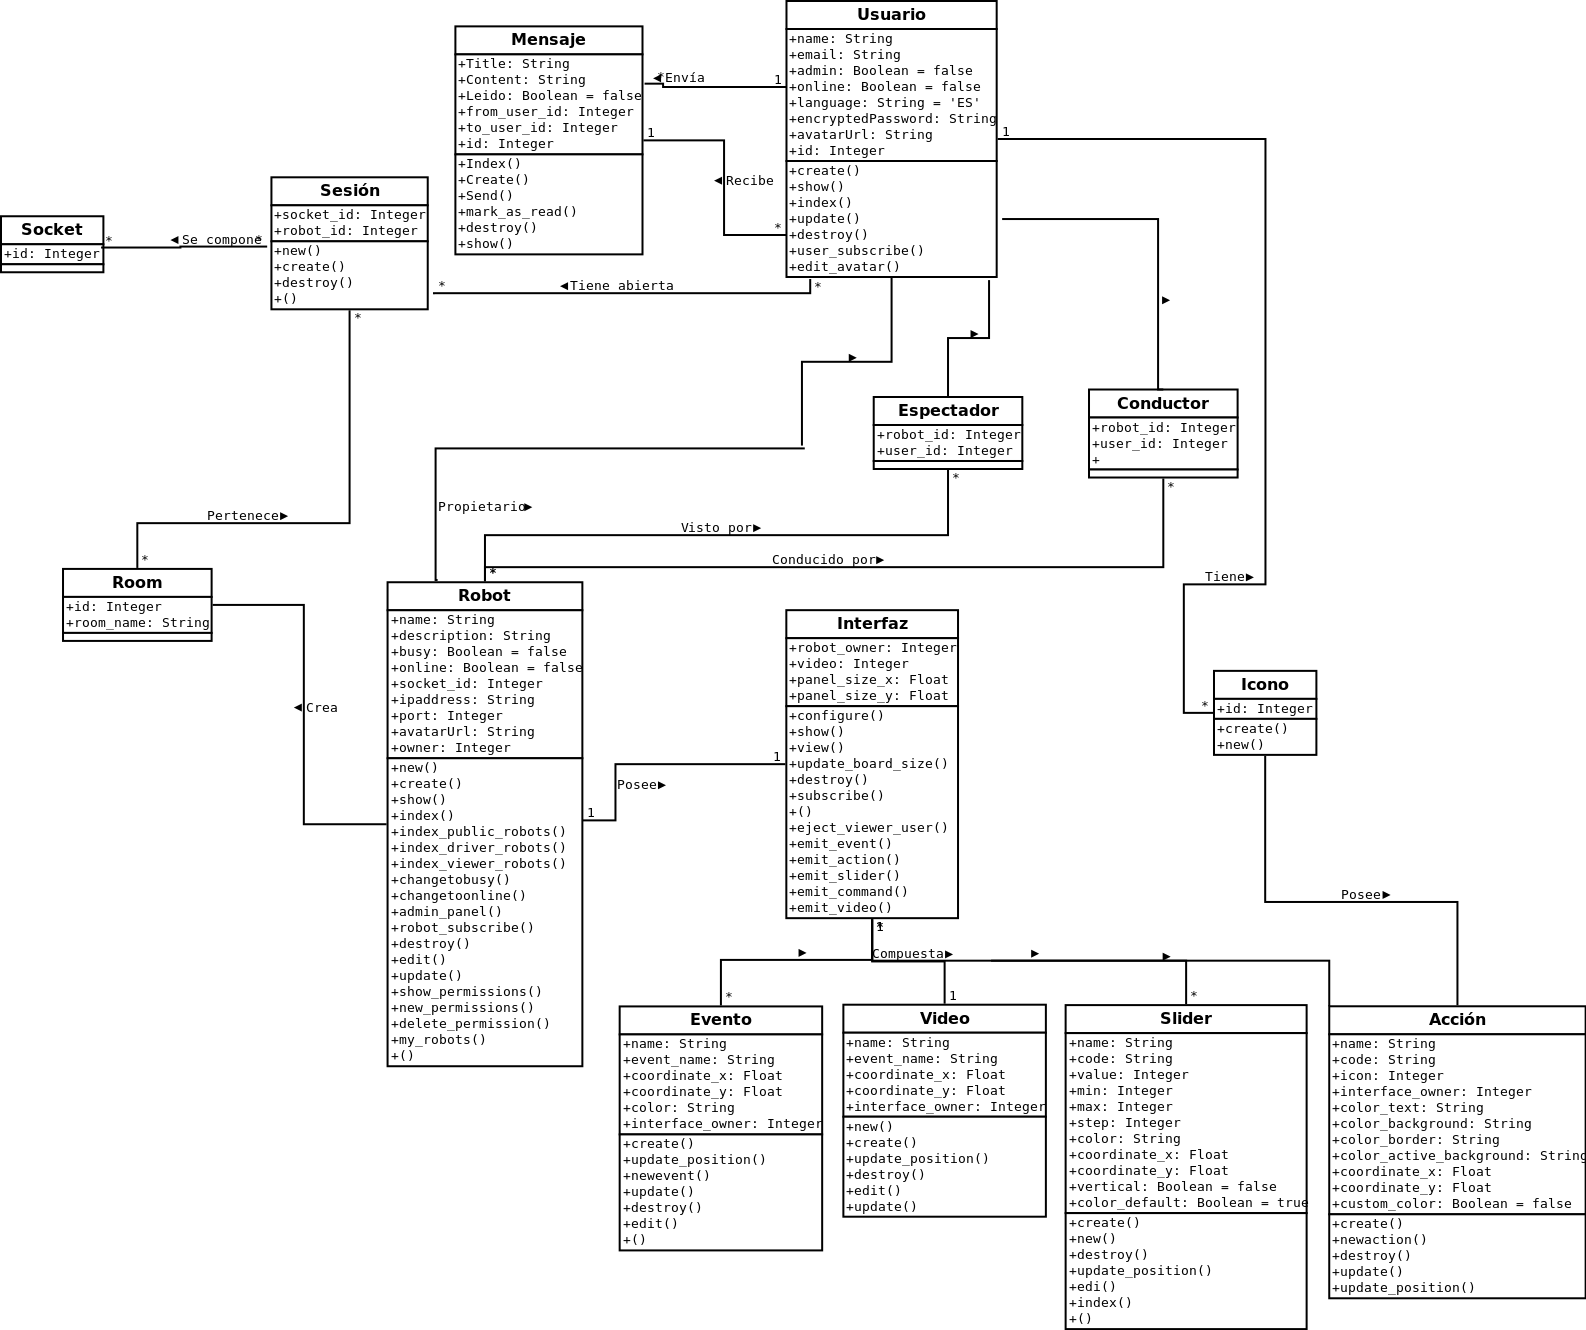
\includegraphics[scale=0.35,angle=270]{diagramas/ModeloUML.png}
  \end{center}
  \caption{Diagrama de clases para la BD.}
  \label{diagram:caso-uso}
\end{figure}



% Este archivo es parte de la memoria del proyecto fin de carrera
% de Manuel López Urbina. Protegida bajo la licencia GFDL.
% Para más información, la licencia completa viene incluida en el
% fichero fdl-1.3.tex

% Copyright (C) 2017 Manuel López Urbina

\chapter{ Desarrollo Frontend }
\label{chap:interfaz-gráfica}

\section {Elementos de la interfaz gráfica}

Para la elaboración de parte referente al front\footnote{ El FrontEnd son todas aquellas tecnologías que corren del lado del cliente, es decir, todas aquellas tecnologías que corren del lado del 
navegador web, generalizándose más que nada en tres lenguajes, Html , CSS Y JavaScript, normalmente el FrontEnd se encarga de estilizar la página de tal manera que la página pueda quedar cómoda 
para la persona que la utiliza transmitiendo una experiencia de usuario cómoda.} de la aplicación se ha empleado Bootstrap, un potente framework CSS que fue creado por Twitter para simplificar el
proceso de maquetación. Este framework CSS presenta multitud de ventajas:

\begin{itemize}
  \item Permite crear interfaces adaptables a los diferentes navegadores, tanto de escritorio como tablets o móviles con distintas escalas y resoluciones.

  \item Se integra perfectamente con las principales librerías Javascript, entre ellas JQuery.

  \item Ofrece un diseño sólido usando LESS y estándares como CSS3/HTML5.

  \item Es un framework ligero y fácilmente integrable en la mayoría de proyectos.

  \item Funciona con los navegadores más populares.

  \item Dispone de distintos layouts predefinidos con estructuras fijas a 940 píxeles de distintas columnas o diseños fluidos.
\end{itemize}

Por otra parte, dada la cantidad de efectos dinámicos necesarios en la aplicación junto con múltiples llamadas Ajax, se ha utilizando jQuery que es un framework Javascript que facilita toda esta
labor haciéndola compatible con los navegadores más comúnmente utilizados.\\

Se consideró antes de comenzar a definir los diferentes estilos y características desarrollo de la interfaz gráfica, una serie de elementos mínimos imprescindibles que dicha interfaz debería incorporar.\\

Dada las características del proyecto, era necesario proporcionar a la aplicación de un entorno gráfico sencillo, intuitivo pero a la vez funcional teniendo como principal objetivo ofrecer al usuario, tras 
una visión rápida, la localización de los diferentes elementos para control del robot y deducir el funcionamiento general de la aplicación.\\

Las vistas principales desarrolladas en la aplicación son los siguientes:

\begin{itemize}
 \item Vista principal de la aplicación.
 \item Panel de administración para el visionado de los usuarios conectados en tiempo real.
 \item Panel de administración para el visionado de los robots conectados en tiempo real.
 \item Formularios de registro de usuarios y robots.
 \item Panel de creación y edición de interfaces de control.
 \item Panel de control de robots.
 \item Panel de visualización de robots.
 \item Índice de robots disponibles.
\end{itemize}


El desarrollo de todos los componentes anteriormente mencionados se han ido realizando paralelamente al desarrollo de la parte Backend\footnote{El BackEnd, en contraposición al FrontEnd
es el área dedicada a la parte lógica de un sitio web, el BackEnd engloba toda la parte no visible para el usuario, excluyendo toda la parte de diseño o de elementos gráficos.} correspondiente.\\


\newpage

\chapter{Comunicaciones}
\label{chap:robot}


En el presente capítulo comenzaremos con una introducción sobre el funcionamiento y los fundamentos teóricos sobre cómo se gestionan las diferentes conexiones y eventos de cualquier aplicación
Sails para, posteriormente, centrarnos específicamente en la descripción de un caso práctico desarrollado en el presente proyecto con la finalidad de comprender mejor su funcionamiento y poder afianzar
conocimientos.


\subsection{Introduccion}
\label{sec:fundamentos}

En esta sección se comenzaremos destacando aquellos aspectos teóricos sobre cómo Sails, framework Node JS utilizado en el desarrollo, trabaja con websocket y socket.io.\\

Como sabemos, un servidor http no puede enviar datos a menos que un cliente los haya solicitado mediante una petición. Los Websockets, en cambio, presentan la particularidad de que
permiten que un servidor envíe datos a un cliente sin la necesidad de que éstos sean solicitados, al menos de una manera inmediata. Estas solicitudes, realizadas con anterioridad, se formalizan mediante suscripciones, concepto que 
iremos constantemente haciendo referencia a lo largo del presente capítulo y que debemos recordar.\\


\begin{figure}%
    \centering
    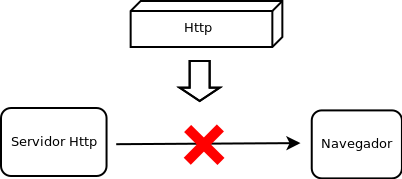
\includegraphics[width=7cm]{diagramas/http-weboscket.png}
    \qquad
    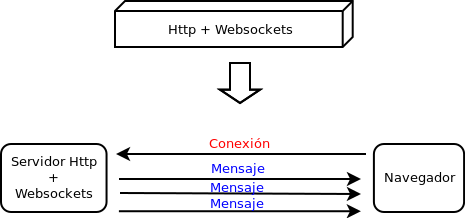
\includegraphics[width=7cm]{diagramas/http+weboscket.png}
    \caption{Peticiones entre un navegador y un servidor http con y sin el empleo de websockets.}%
    \label{fig:http-request}%
\end{figure}

Anteriormente comentamos que el servidor http no puede enviar datos a menos que el cliente lo haya solicitado y los Websockets permiten que un servidor envíe datos no solicitados una vez que se hace 
una conexión inicial (suscripción) desde el lado del cliente. Una aplicación Sails típica queda dividida en dos partes. La primera, en el lado del servidor, consta de un servidor http junto con un nodo
central que actúa como un servidor de sockets.\\ 

En segundo lugar, en el lado del cliente, se dispone de los diferentes códigos html y funciones JavaScript para realizar las conexiones con el servidor. Estas conexiones cliente-servidor permiten que 
cualquier otro cliente conectado pueda enviar mensajes al servidor para que a su vez éstos sean emitidos a los clientes que se encuentren conectados en la aplicación en ese instante.\\

Además cada socket posee un identificador único que identifica de manera inequívoca el cliente o, en nuestro, caso el navegador que está accediendo a la página.\\

Destacar también el concepto de salas o rooms de Socket.io. Las salas nos permite agrupar los sockets de modo que en lugar de mensajes que son enviados a todos los sockets conectados, se puede enviar mensajes
sólo a los sockets que están asociados con una sala. De esta podremos mandar mensajes específicos para un cliente concreto, todos ellos o un conjunto de los mismos. \\


\begin{figure}[H]
  \begin{center}
    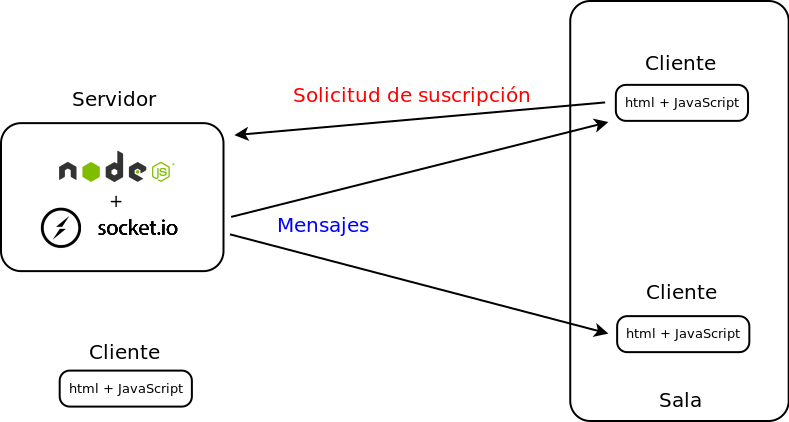
\includegraphics[scale=0.35]{diagramas/salas-websocket.png}
  \end{center}
  \caption{Representación de una sala compuesta por dos clientes.}
  \label{view:userindex}
\end{figure}


De todo los anterior podemos deducir que Sails es un framework especialmente potente, el cual proporciona infinidad de posibilidades a desarrollar. A continuación se cita un fragmento tal y 
como podemos extraer de la página oficial de Sails:\\

\begin{center}
\emph{Sails.js facilita el desarrollo de aplicaciones Node.js empresariales. Ha sido diseñado para imitar el patrón MVC de frameworks como Ruby on Rails, pero con soporte para los requisitos de aplicaciones modernas: data-driven APIs con una arquitectura escalable y service-oriented. Es especialmente bueno para el desarrollo de chats, cuadros de mando en tiempo real o juegos multijugadores.} 
\end{center}


En este caso menciona diferentes aplicaciones tipo que pueden desarrollarse con Sails, desde un chat, cuadros de mando en tiempo real o juegos multijugadores. RobotUI resulta como una combinación de las 
anteriores puesto que incorpora cuadros de mandos, sistema de mensajería y también es considerado como un juego ya que también está enfocado al entretenimiento.\\





\subsection{ Comunicaciones en RobotUI }
\label{sec:comunicaciones-robotui}



Tras la comprensión de los fundamentos teóricos descritos en el punto \ref{sec:fundamentos} donde se recogen los fundamentos del framework y sabiendo cómo trabaja y gestiona los sockets pasamos
a trasladarlos a un caso práctico describiendo una de las funcionalidades del proyecto de tal manera que se facilite su comprensión.\\

Como sabemos, Sails nos ayuda a incorporar funcionalidades en tiempo real a nuestra aplicación web. Sails gestiona los eventos aplicándolos sobre los modelos. Comenzamos realizando una descripción
del ejemplo a desarrollar.\\

Centrémonos en el modelo \emph{Usuario} de RobotUI. Uno de los atributos de este modelo es un booleano \emph{online}, el cual representa si un usuario se encuentra logueado en el sistema o no. El objetivo 
es saber cuando el usuario cambia el estado para poder proporcionar una actualización en tiempo real de la página de gestión de usuarios \ref{view:userindex} de manera que cuando usuario inicie sesión o salga de la 
aplicación se alterne entre las imágenes online: \icontext{.2}{.35}{imagenes/comunicaciones/online.png} y offline: \icontext{.2}{.35}{imagenes/comunicaciones/offline.png} sin necesidad de refrescar la página manualmente.\\

\begin{figure}[H]
  \begin{center}
    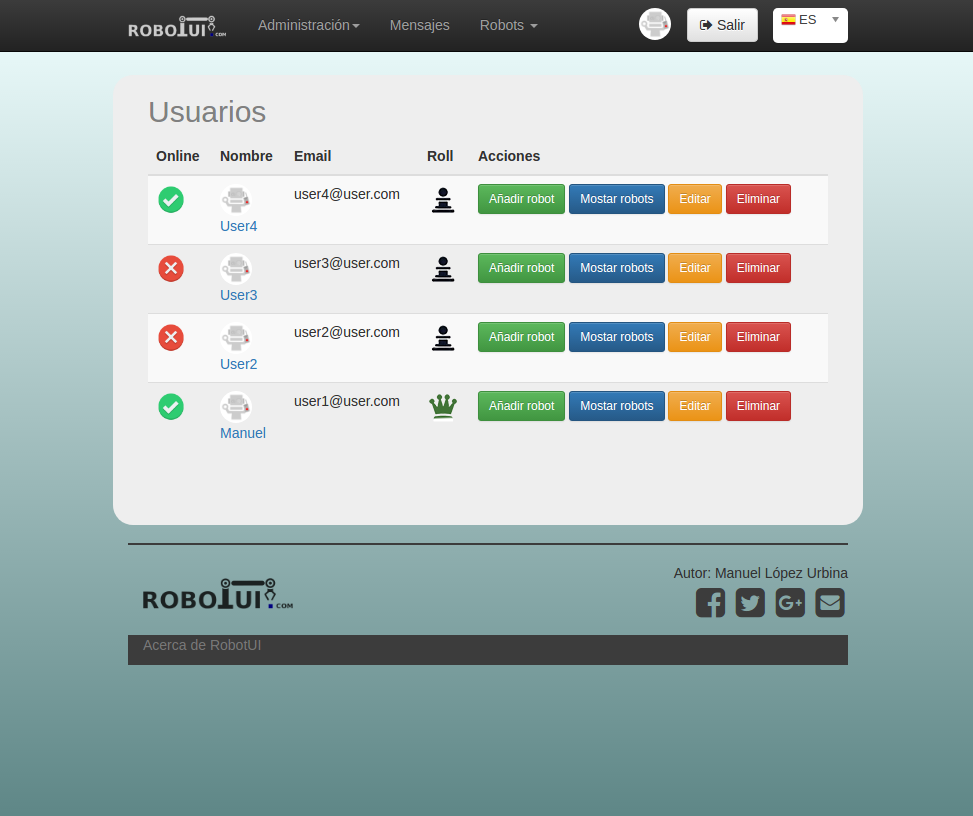
\includegraphics[scale=0.35]{imagenes/comunicaciones/index-usuarios.png}
  \end{center}
  \caption{Página de gestión de usuarios actualizable en tiempo real.}
  \label{view:userindex}
\end{figure}

Para capturar los eventos correspondientes al modelo \emph{Usuario} o cualquier otro debemos realizar una suscripción. Sails incorpora dos modalidades de suscripción. suscripción a clase y 
suscripción a modelo.\\

¿Cuál es la diferencia entre suscribirse a una ``clase'' frente a la suscripción a una ``instancia''? Al suscribirse a la ``clase'' del modelo, el socket podrá escuchar la creación de 
nuevas instancias de modelo mediante un método denominado publishCreate(). Mientras que la suscripción a ``instancia'' permite al socket escuchar los cambios de modelos
a través de los métodos publishUpdate y/o publishDestroy de una instancia o conjunto de instancias en concreto.\\


Por tanto, centrándonos en el ejemplo de los usuarios, debemos realizar la suscripción mediante la definición de una acción en el controlador de usuario. La acción se denominará \emph{user\_subscribe}.\\

En dicha acción podremos acceder al socket solicitante vía req.socket. Así que, primeramente se realiza una suscripción a la sala de ``clase'' del usuario mediante User.watch y pasando 
req.socket como argumento. De esta manera nos hemos suscrito a la clase del modelo de usuario.\\

Seguidamente se realiza la suscripción a las instancias del modelo de usuario mediante el método User.subscribe pasando como parámetro el socket solicitante obtenido a través de req.socket seguido
de un segundo argumento, que son las instancias existentes de usuarios. Las instancias de los usuarios existentes son recuperadas mediante un método de búsqueda para que, posteriormente, su salida 
sea pasada al método de suscripción como segundo argumento. Con esto ya nos hemos suscrito a las salas de instancias del modelo de usuario.\\

A continuación mostramos el código que realiza la suscripción al modelo Usuario en sus dos modalidades, suscripción a modelo y suscripción a instancias de modelo descrito anteriormente:

\begin{lstlisting}[language=JavaScript]

  user_subscribe: function (req, res, next) {
    if (req.isSocket) {
      //Update, destroy...
      User.find(function foundUsers(err, users) {
        if (err) return res.badRequest(err);

        User.subscribe(req.socket, users);
      });

      //Create
      User.watch(req);
      console.log('User ' + req.session.User.id + 'with socket id ' + sails.sockets.id(req) + ' is now subscribed to the model class \'User\'.');
    } else {
      res.view();
    }
  }
  
\end{lstlisting}

Ahora bien, ya nos encontramos suscritos a un modelo, pero... ¿Qué ocurre con publishCreate, publishUpdate y publishDestroy?, ¿Dónde se realiza la llamada a estos métodos?\\


Para ello solamente debemos llamar al método en la acción deseada, por ejemplo, al crear una sessión, tan solo debemos actualizar el usuario como online y mandar el mensaje correspondiente mediante
el método publishUpdate:\\

\begin{lstlisting}[language=JavaScript]

        //Cambio de estado a online
        User.update(user.id, {online: true, longitude: long, latitude: lat}, function (err){
          if (err) return next(err);

          //Informar a otros clientes (sockets abiertos) que el usuario esta logueado
          User.publishUpdate(user.id, {
            loggedIn: true,
            id: user.id
          });
         });

\end{lstlisting}


Del mismo modo para publishCreate o publishDestroy.\\


¿Y desde el lado del cliente? ¿Cómo realizamos las llamadas a las diferentes acciones de suscripción y cómo capturamos los eventos?\\


Las siguientes funciones resultan de vital importancia:\\

\begin{lstlisting}[language=JavaScript]


<script type="text/javascript">

  $.when(savesocket()).done(function(){
    if (typeof subscribeAndListen == 'function') {
      subscribeAndListen();
    }
    listenMessages();
  });

  //Funcion para tener en to do momento almacenado en la tabla session los sockets conectados junto con el usuario al que pertenece
  function savesocket() {
    io.socket.get("/session/saveSocketID");
  }
</script>

\end{lstlisting}


Primeramente tenemos la función \emph{savesocket} la cual realiza la llamada al método saveSocketID del controlador \emph{session}. Dicho método realiza el registro en base de datos ligando el identificador del 
socket abierto con el usuario al que corresponde, de tal manera que siempre sabremos qué socket corresponde con qué usuario.

\begin{lstlisting}[language=JavaScript]


  //Almacenamiento en la base de datos la sesion de cada usuario de la pagina
  saveSocketID: function(req, res) {
    if (!req.isSocket) return res.badRequest();

    var socketId = sails.sockets.id(req);
    // => "BetX2G-2889Bg22xi-jy"

    var sessionObj = {
      socket_id: socketId,
      user_id: req.session.User != undefined ? req.session.User.id : null
    };

    Session.create(sessionObj).exec( function (err, session) {
      if (err) return res.badRequest();

      console.log('\n....................................................');
      console.log('Conectando a Sails js...');
      console.log('Cliente conectado - id del socket: ' + socketId);
      console.log('....................................................');

      return;
    });
  }
  
\end{lstlisting}

Una vez tenemos almacenado el par socket-usuario buscamos la función subscribeAndListen, la cual será específica según la vista en la que nos encontremos, por ejemplo, si nos encontramos en el panel
de administración de usuarios, la función subscribeAndListen será específica para 


\begin{lstlisting}[language=JavaScript]


<script type="text/javascript">

  function subscribeAndListen() {
    io.socket.get('/user/user_subscribe');

    io.socket.on('user', function (obj) {
      if (obj.verb == 'created') {
        var user = obj.data;
        $.ajax({
          url: '/user/render',
          type: 'GET',
          data: {id: user.id},
          success: function(data){
            $("#user_list").append(data);
           toastr.info('<%= i18n('user_created')%>', 'RobotUI' )
          }
        });
      }

      if (obj.verb == 'updated') {
        var data = obj.data;
        change_img_state(data.id, data.loggedIn, '<%= i18n('connect')%>', '<%= i18n('disconnect')%>');

        if (data.id != '<%= req.session.User.id %>') {
          if (data.loggedIn) {
           toastr.info('<%= i18n('user_connected')%>', 'RobotUI');
          } else {
           toastr.info('<%= i18n('user_disconnected')%>', 'RobotUI');
          }
          console.log('User has been updated to online:' + data.loggedIn);
        }
      }

      if (obj.verb == 'destroyed') {
        $("#user_" + obj.id).remove();
       toastr.info('<%= i18n('user_destroyed') %>', 'RobotUI' );
      }

    });

  }

</script>

\end{lstlisting}





\begin{figure}[H]
  \begin{center}
    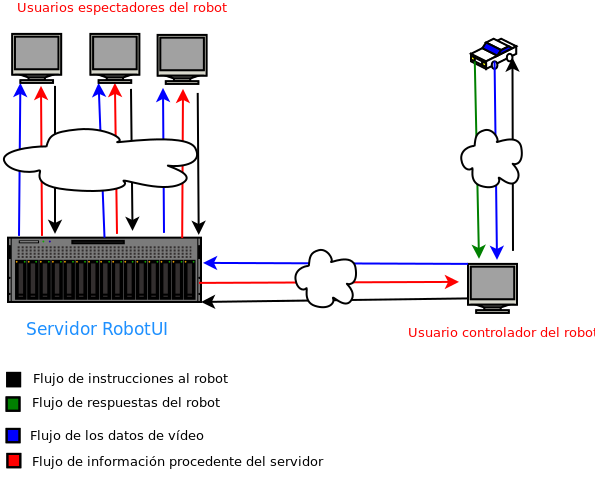
\includegraphics[scale=0.5]{diagramas/flujo-comunicaciones.png}
  \end{center}
  \caption{Esquema representativo del flujo de conexiones de RobotUI.}
  \label{diagram:conexiones}
\end{figure}

\subsubsection{ Conexión }
\label{sec:conexion}


Cuando se realiza una una conexión de un usuario al sistema, un nuevo cliente, realiza una petición al servidor, el cual captura la llamada y renderiza la vista correspondiente elaborando una respuesta.\\

Dicha respuesta se corresponde con el cógido Html y JavaScript que recibe el navegador. En el archivo \emph{views/layout.js} se encuentra el siguiente código JavaScript de gran importancia
para el funcionamiento de toda la aplicación por lo que resulta interesante su comprensión.\\

Primeramente al realizarse una nueva conexión de un cliente en el sistema el servidor debe conocer y registrar a dicho cliente con la finalidad de seguir su comportamiento, sus acciones y 
movimientos por toda la aplicación.\\

\begin{lstlisting}[language=JavaScript]
  \/\/Funcion para tener en todo momento almacenado en la tabla session los sockets conectados junto con el usuario al que pertenece
  function savesocket() {
    io.socket.get("/session/saveSocketID");
  }  
\end{lstlisting}


Función que realiza el registro de un nuevo cliente en la base de datos:\\

\begin{lstlisting}[language=JavaScript]


  //Almacenamiento en la base de datos la sesion de cada usuario de la pagina
  saveSocketID: function(req, res) {
    if (!req.isSocket) return res.badRequest();

    var socketId = sails.sockets.id(req);
    // => "BetX2G-2889Bg22xi-jy"

    var sessionObj = {
      socket_id: socketId,
      user_id: req.session.User != undefined ? req.session.User.id : null
    };

    Session.create(sessionObj).exec( function (err, session) {
      if (err) return res.badRequest();

      console.log('\n....................................................');
      console.log('Conectando a Sails js...');
      console.log('Cliente conectado - id del socket: ' + socketId);
      console.log('....................................................');

      return;
    });
  },

\end{lstlisting}

Una vez finaliza el registro en el servidor del nuevo cliente se comprueba si existe definida la función \emph{ subscribeAndListen } llamándose en caso afirmativo. Dicha función es específica para cada
funcionalidad que queramos inicializar o a qué eventos nos deseemos suscribir. Por ejemplo, suscribirnos a los eventos de conexión y desconexión de usuarios del panel de administración descrito en el apartado
\ref{sec:fundamentos} mediante la definición de la función \emph{subscribeAndListen} en la vista correspondiente.\\


Por otro lado, siempre se realiza la llamada a la función \emph{listenMessages} ya que independientemente de la vista en la que nos encontremos siempre nos mantendremos a la escucha de los mensajes 
recibidos a nuestra bandeja de entrada por parte de otros usuarios.\\

Finalmente mostramos el código JavaScript al completo localizado en el archivo \emph{views/layout.js}:\\


\begin{lstlisting}[language=JavaScript]

<script type="text/javascript">

  $.when(savesocket()).done(function(){
    if (typeof subscribeAndListen == 'function') {
      subscribeAndListen();
    }
    listenMessages();
  });

  //Funcion para tener en todo momento almacenado en la tabla session los sockets conectados junto con el usuario al que pertenece
  function savesocket() {
    io.socket.get("/session/saveSocketID");
  }

</script>
 
\end{lstlisting} 
 
\subsubsection { Desconexión }
\label{sec:deconexion}

En este apartado describiremos los puntos de mayor relevancia a la hora de la desconexión de alguna de las diferentes comunicaciones establecidas comenzando con la desconexión de un usuario.\\

Cuando un usuario realiza una desconexión, bien deslogueándose de la página o cerrando una de las ventanas abiertas, automáticamente se lanza una llamada a la 
función \emph{afterDisconnect} localizada en el fichero \emph{config/Socket.js} del servidor. Función que será ejecutada cada vez que un socket es desconectado del sistema.\\

Dicha función primeramente localiza qué sesión en la base de relacionada está relacionada con identificador del socket desconectado. Si este socked estaba usando algún robot, éste se libera cambiando el estado
del robot a \emph{libre}. Y se informa a todos los sockets abiertos que el robot queda libreado y accesible al resto de usuarios.\\

\begin{lstlisting}[language=JavaScript]
  Robot.update({id: session.robot_id}, {busy: false}, function robotUpdated(err) {
    if (err) return next(err);

    //Informar a otros clientes (sockets abiertos) que el robot queda liberado
    Robot.publishUpdate(session.robot_id, {
      busy: false,
      id: session.robot_id
    });
  });
\end{lstlisting}


A continuación, se comprueba si el usuario no dispone de más sockets abiertos. Si fuera el caso de que no los disponga, entonces se procede a cambiar su estado a desconectado y se emite o se informa al resto de clientes (sockets abiertos)
que el usuario ya no se encuentra en el sistema. Llamada al método \emph{User.publishUpdate}: \\

\begin{lstlisting}[language=JavaScript]
   User.publishUpdate(session.user_id, {
    loggedIn: false,
    id: session.user_id
  });
\end{lstlisting}


Se comprueba si el usuario desconectado se encontraba en alguna \emph{room}. Pongamos como ejemplo que el usuario ha abandonado la visualización de un robot por lo queda
se debe informar a todos los sockets integrantes de esa \emph{room} que un usuario la ha abandonado con la función \emph{ sails.sockets.broadcast }. A continuación se muestra el fragmento de código:\\


\begin{lstlisting}[language=JavaScript]

//Emite a cada room que que se encuentre la sesión que un usuario la ha abandonado

session.rooms.forEach(function (room) {
  //sails.sockets.leave(session.socket_id, room.room_name, function(err) {
  //  if (err) {return res.serverError(err);}
  //});
  sails.sockets.broadcast(room.room_name, {type: 'exit', msg: {user_id: session.user_id}});
});

\end{lstlisting}



Finalmente se destruye la sesión:\\

\begin{lstlisting}[language=JavaScript]
    Session.destroy(session.id, function sessionDestroyed(err) {
      if (err) return cb();
      return cb();
    });
\end{lstlisting}


A continuación mostramos el código completo de la función \emph{afterDisconnect}:\\


\begin{lstlisting}[language=JavaScript]

  afterDisconnect: function(session, socket, cb) {
     console.log('Cliente desconectado - id del socket: ' + socket.id);

    //Session del socket cerrado,
    Session.findOne({socket_id: socket.id}).populate('rooms').exec(function (err, session) {
      if (err) return cb();
      if (!session) return cb();

      //Comprobar si el soscket estaba usando algun robot para liberarlo:
      if (session.robot_id) {
        console.log('Socked was using a robot');

        Robot.update({id: session.robot_id}, {busy: false}, function robotUpdated(err) {
          if (err) return next(err);

          //Informar a otros clientes (sockets abiertos) que el robot queda liberado
          Robot.publishUpdate(session.robot_id, {
            busy: false,
            id: session.robot_id
          });
        });
      }


      //Emite a cada room que que se encuentre la sesión que un usuario la ha abandonado ->  
      session.rooms.forEach(function (room) {
        //sails.sockets.leave(session.socket_id, room.room_name, function(err) {
        //  if (err) {return res.serverError(err);}
        //});
        sails.sockets.broadcast(room.room_name, {type: 'exit', msg: {user_id: session.user_id}});
      });


      //Comprobar si el usuario tiene más sockets abiertos:
      Session.count({user_id: session.user_id}).exec(function countUserSessions(error, n_sessions) {
        console.log('There are ' + n_sessions + ' users ' + session.user_id);

        //Cambiamos el usuario a offline si solo tenía una ventana o conexión abierta.
        if (n_sessions == 1) {
          User.update(session.user_id, {online: false}, function (err) {
            if (err) return cb(err);

            //Informar a otros clientes (sockets abiertos) que el usuario ya NO se encuentra logueado
            User.publishUpdate(session.user_id, {
              loggedIn: false,
              id: session.user_id
            });
          });
        }

        Session.destroy(session.id, function sessionDestroyed(err) {
          if (err) return cb();
          return cb();
        });
      });
    });
  }

\end{lstlisting}
 

\chapter{Robot de pruebas}
\label{chap:robot}

Con la finalidad de demostrar y hacer un primer uso de la aplicación RobotUI se ha decidido abordar la elaboración de un vehículo de pruebas. Dicho vehículo será utilizado de modelo o guía para el 
resto de personas que quieran crear un robot para su integración en la aplicación o bien para programar un robot del que ya dispongan previamente.\\

En el presente capítulo se detalla los diferentes pasos que se han seguido a la hora de la construcción y programación del vehículo desarrollado. Este capítulo tiene como objetivo proporcionar al usuario
una guía básica a partir de la cual poder desarrollar sus propios robots e integrarlos en la aplicación RobotUI.\\


\begin{figure}[H]
  \begin{center}
    \includegraphics[scale=0.2]{imagenes/robot2.jpg}
  \end{center}
  \caption{Imagen del robot de pruebas desarrollado.}
  \label{robot:robot02}
\end{figure}


\section{Análisis}
\label{sec:analisis}

\subsection{Análisis de requerimientos hardware}
\label{sec:requerimientos-hardware}

Se ha optado por la construcción de un  pequeño robot móvil dotado de un chasis de 4 ruedas donde cada una de ellas está accionada por un motor. Los motores seleccionados deberán funcionar a 
corriente continua de manera que en función de la polarización de los terminales haga girar las ruedas en una dirección o la contraria (marcha adelante o atrás).\\

El chasis utilizado deberá permitir añadir multitud de componentes necesarios para construir el robot, deberá disponer de paneles para instalar las diferentes
placas electrónicas y sensores.\\

El robot además necesita de una cámara para la obtención de vídeo y su transmisión siendo necesaria una cámara de pequeñas dimensiones de alta definición.\\

Por otra parte, todo robot necesita de una unidad de central de procesamiento donde se localizará el programa de control. Este programa tendrá la función de interpretar las diferentes señales recibidas,
control de sensores y dispositivos conectados. Además, esta placa es la encargada de distribuir la alimentación por los diferentes componentes hardware que lo necesiten y recibir las señales de
los sensores y enviarla a los motores. Utilizando para ello la placa Raspberry Pi modelo B cuya descripción se encuentra en la sección \ref{sec:raspberry}.\\

Este modelo de placa dispone de  una serie de pines denominados GPIO (General Purpose Input/Output) que son, como su propio nombre indica, un sistema de E/S (Entrada/Salida) de propósito general,
es decir, una serie de conexiones que se pueden usar como entradas o salidas para usos múltiples. Estos pines están incluidos en todos los modelos de Raspberry Pi, con la
finalidad de ser utilizados en diferentes proyectos de una manera similar a la que se haría con Arduino\footnote{Arduino es una plataforma de prototipos electrónica de código abierto (open-source) 
basada en hardware y software flexibles y fáciles de usar.}.

\section{Análisis de requerimientos de Software}

Habiendo detallado los requerimientos hardware para la construcción del robot, pasamos al análisis de los diferentes requerimiento software para la correcta
gestión de los diferentes elementos hardware y para su correcto funcionamiento.\\

En cuanto a la programación del robot, uno de los requisitos fundamentales es el de disponer de una vía de comunicación bidireccional.\\

Para ello se ha seleccionado el entorno de ejecución Node.Js, el cual permite escribir programas en JavaScript además de disponer de una gran cantidad de bibliotecas hechas por toda una comunidad que la respalda.
Además de que permite escribir programas relativamente complejos en tan sólo unas pocas líneas de código.\\

se ha realizado haciendo uso de Websockets los cuales presentan algunas ventajas sobre simples solicitudes http:

\begin{itemize}
 \item Velocidad: Una petición http normal tiene que establecer una conexión antes de comenzar las transacciones, la cual toma bastante tiempo. 
 Los Websockets, una vez establecida la conexión, siempre están abiertos y listos para enviar o recibir datos. Esto significa que el retraso puede ser tan bajo como su ping,
 en torno a un milisegundo o dos en la mayoría de los casos.
 \item Bidireccional: Los Websockets permiten transmisión de datos en ambas direcciones permitiendo la activación de eventos en el cliente y viceversa.
\end{itemize}

Como podemos ver las propiedades anteriormente descritas resultan esenciales para nuestro proyecto que, como cabe recordar, queremos realizar lectura de sensores y envío de órdenes desde un servidor 
externo. Además de la transmisión de vídeo.\\

\section{Montaje}

En esta sección se recogen todas las descripciones y procedimientos seguidos y que han resultado de mayor interés a la hora de la construcción del robot y sus diferentes interconexiones.\\

\subsection{Interconexión de elementos}

En el presente punto, se recoge todos aquellos puntos de interés referentes a la interconexión de elementos utilizados, los cuales quedaron descritos en la sección \emph{Tecnologías hardware}
\ref{sec:tecnologias-hardware} junto con sus especificaciones.\\

Comenzando por el módulo central del sistema, la placa Raspberry Pi Model B+, dispone de una serie de pines denominados GPIO (General Purpose Input/Output) es, como su propio nombre indica, 
un sistema de E/S (Entrada/Salida) de propósito general, es decir, una serie de conexiones que se pueden usar como entradas o salidas para usos múltiples. Estos pines se encuentran en todos
los modelos de Raspberry Pi.\\

Los GPIO representan la interfaz entre la Raspberry Pi y el mundo exterior. En este caso para el control de los motores del vehículo.\\

Primeramente, antes de comenzar a utilizarlos debemos conocer sus características y como están distribuidos en nuestra placa. los pines GPIO para la Raspberry Pi 3 Model B, se encuentran distribuidos 
de la siguiente manera:

\begin{figure}[H]
  \begin{center}
    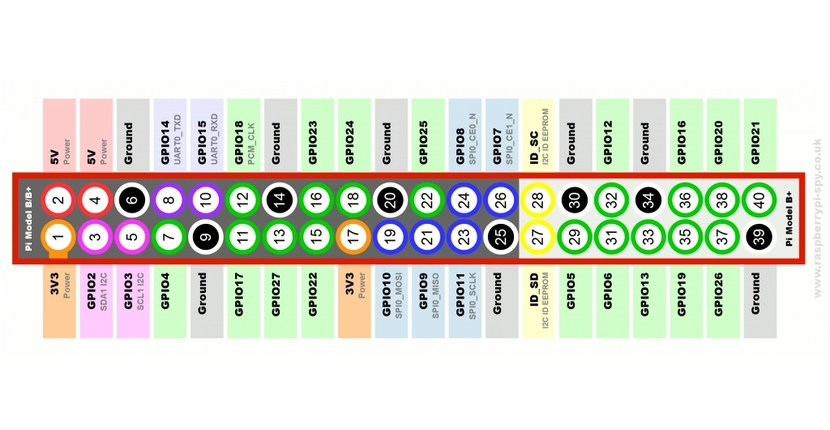
\includegraphics[scale=0.4]{imagenes/robot/gpio-conexiones.jpg}
  \end{center}
  \caption{Esquema GPIO de una Raspberry Pi Model B+.}
  \label{gantt:tareas01}
\end{figure}

Los pines empleados son los siguientes para la construcción del robot han sido los siguientes:\\

\begin{table}[H]
  \begin{center}
    \begin{tabular}{|p{2.5cm}|p{2.5cm}|p{4.5cm}|}
      \hline
      {\textbf{GPIO}} & \textbf{ Modo } & \textbf{ Control }\\
      \hline
      {\textbf{ 2 }} & { OUTPUT } & { Motores lado izquierdo }  \\
     \hline
      {\textbf{ 3 }} & { OUTPUT } & { Motores lado izquierdo } \\
      \hline
      {\textbf{ 17 }} & { OUTPUT } & {  Motores lado derecho } \\
      \hline
      {\textbf{ 27 }} & { OUTPUT } & { Motores lado derecho } \\
     \hline   
    \end{tabular}
  \end{center}
\caption{ Tabla con los puertos GPIO utilizados, su configuración establecida y su utilización. }
\end{table}


Pero existe una problemática y es que no podemos conectar directamente los pines de salida de nuestra placa Raspberry Pi directamente a los motores. Esto es debido a
que la placa no dispone de potencia suficiente para mover actuadores. De hecho, la función de la placa no debe ser ejecutar acciones sino mandar ejecutar acciones a drivers que realicen
el trabajo pesado.\\

Para ello empleamos el L298N, un controlador (driver) de motores, el cual nos permite encender y controlar dos motores de corriente continua desde una Raspberry Pi, Arduino o cualquier placa similiar,
variando tanto la dirección como la velocidad de giro.\\

La corriente máxima que el L298N puede suministrar a los motores es, en teoría, 2A por salida (hasta 3A de pico) y una tensión de alimentación de 3V a 35V. Sin embargo, el L298N tiene una 
eficiencia baja. La electrónica supone una caída de tensión de unos 3V, es decir, la tensión que recibe el motor es unos 3V inferior a la tensión de alimentación.\\

Estas pérdidas se disipan en forma de calor lo que se traduce en que, a efectos prácticos, es difícil que podamos obtener más de 0.8-1A por fase sin exceder el rango de temperatura de funcionamiento.\\

El L298N incorpora protecciones contra efectos que pueden producirse al manejar motores de corriente continua. Dispone de protecciones contra sobre intensidad, sobre temperatura, y diodos de protección
contra corrientes inducidas.\\

El módulo seleccionado, el cual incorpora el controlador L298N, cuenta con todos los componentes necesarios para funcionar sin necesidad de elementos adicionales, entre ellos diodos de protección
y un regulador \textbf{LM7805} que suministra 5V a la parte lógica del integrado L298N. Además cuenta con jumpers de selección para habilitar cada una de las salidas del módulo (A y B).
La \textbf{salida A} esta conformada por \textbf{OUT1} y \textbf{OUT2} y la \textbf{salida B} por \textbf{OUT3} y \textbf{OUT4}. Los pines de habilitación son \textbf{ENA} y \textbf{ENB} respectivamente.\\

En la figura \ref{diagrama:L298N-salidas} se muestra el módulo empleado con sus diferentes pines al detalle.\\


\begin{figure}[H]
  \begin{center}
    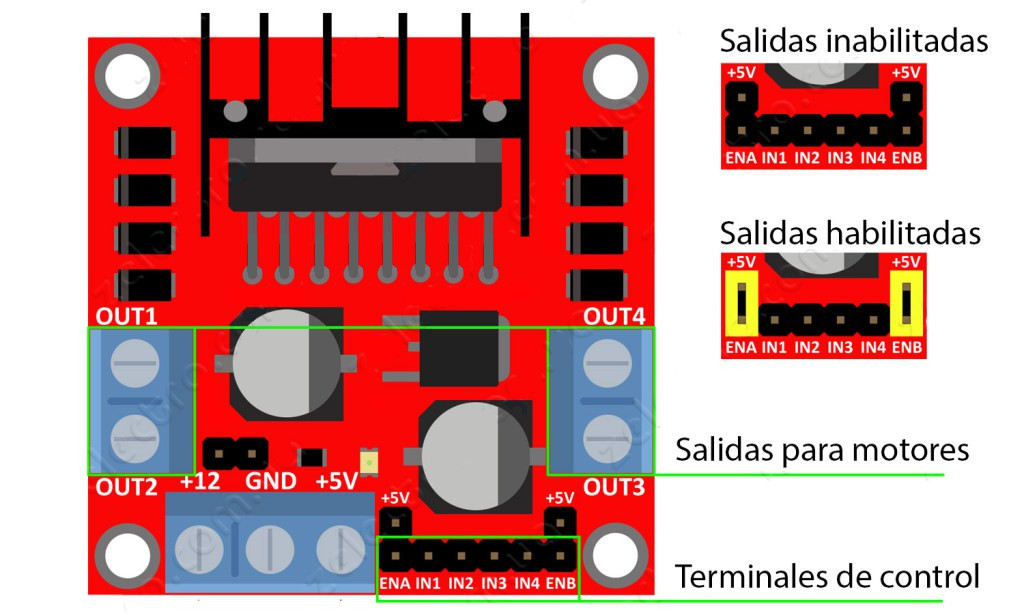
\includegraphics[scale=2.5]{imagenes/L298N-conexiones.jpg}
  \end{center}
  \caption{Pines de entrada/salida del módulo L298N empleado.}
  \label{diagrama:L298N-salidas}
\end{figure}

\subsubsection{Alimentación}

Para la alimentación del conjunto se ha optado por la utilización de dos baterías. Una para dotar de energía a la placa de control y otra para la alimentación de los motores debido a la gran cantidad de energía 
que éstos demandan y su elevado consumo.\\

Para la alimentación de la placa Raspberry Pi, se ha optado por la utilización de una batería de Litio desarrollada específicamente para su uso con este modelo de placas el cual permite una integración
perfecta. Dicho módulo de alimentación queda descrito en la subapartado correspondiente de herramientas utilizadas \ref{componente:bateria-expansion}.

Imagen de la Raspberry Pi junto con su módulo de expansión de batería:

\begin{figure}[H]
  \begin{center}
    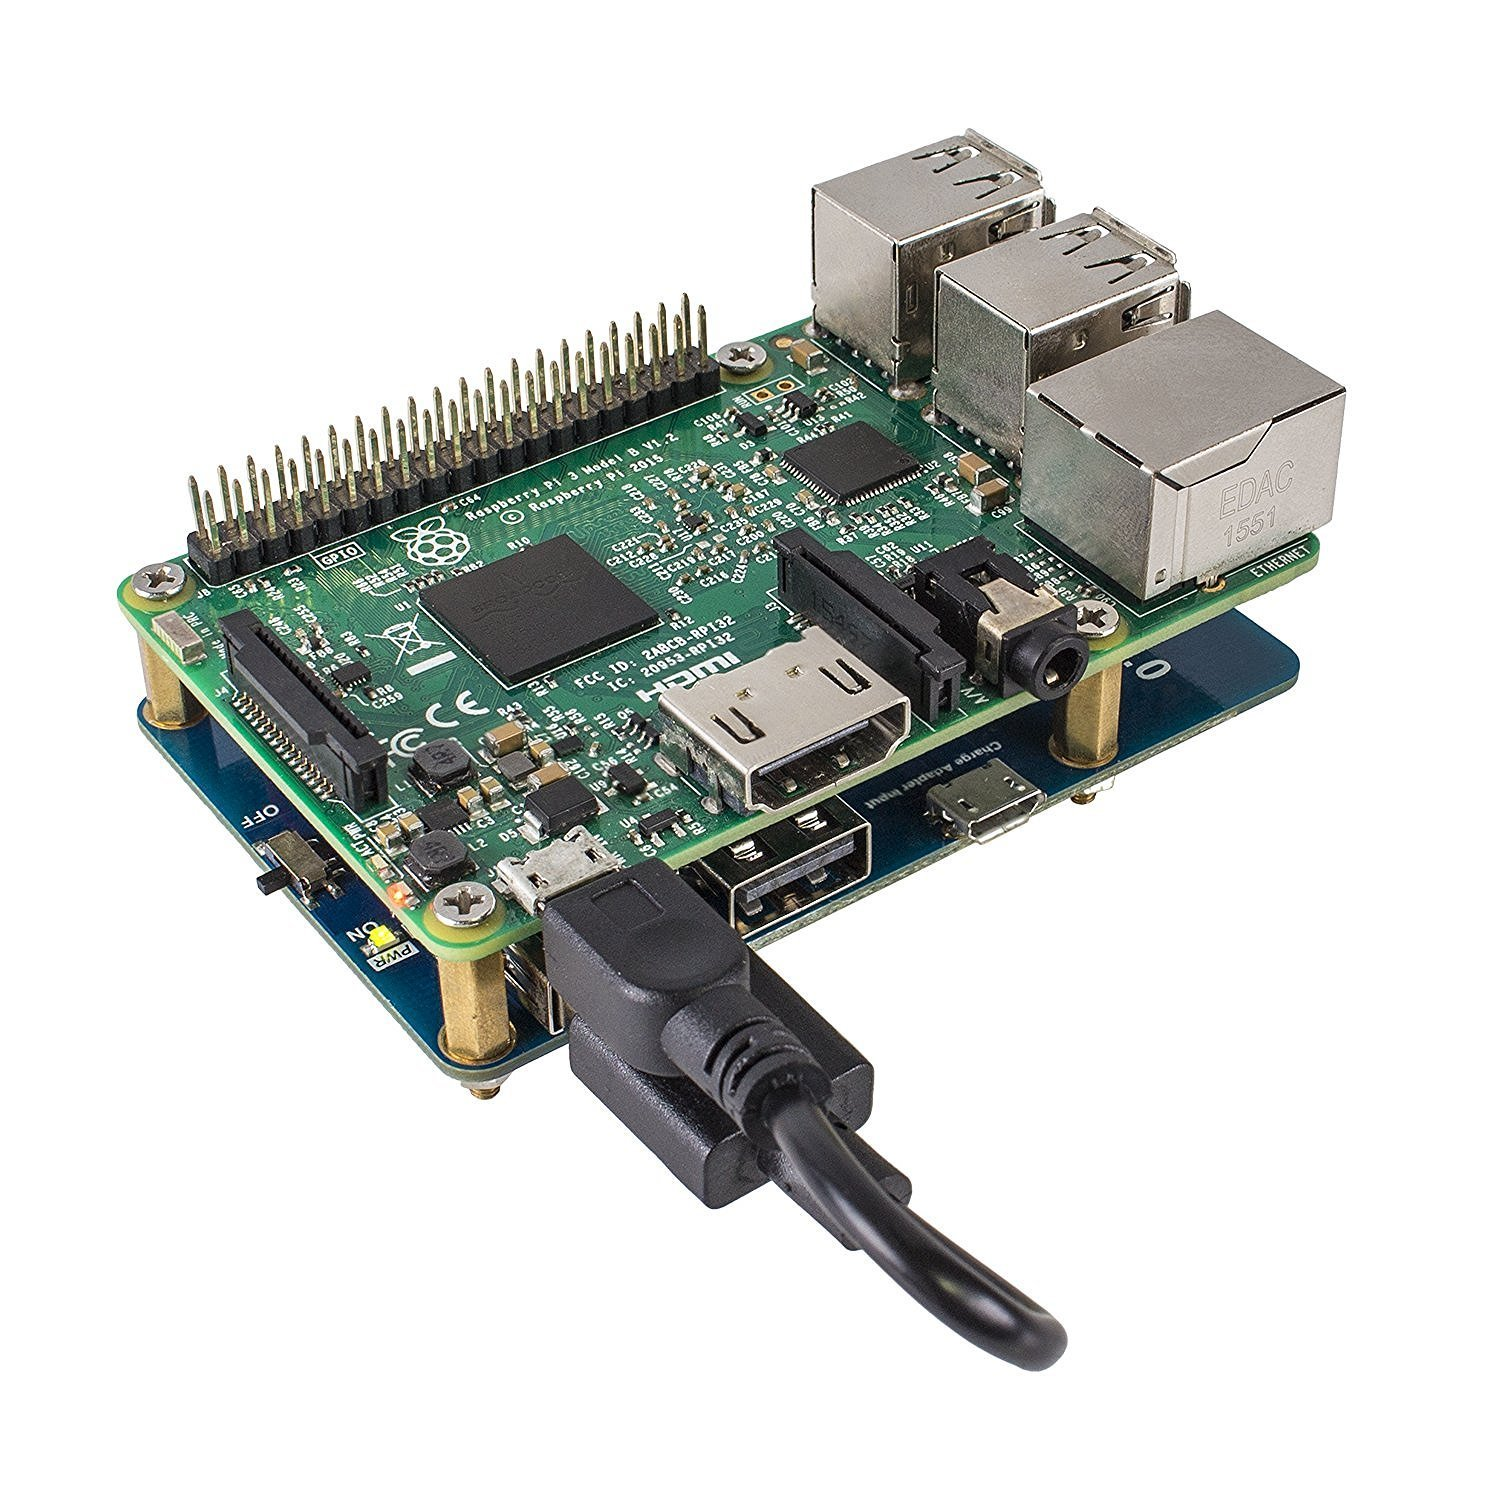
\includegraphics[scale=0.15]{imagenes/modulo-expansion-rpi.jpg}
  \end{center}
  \caption{Conjunto Raspberry Pi y módulo de expansión de alimentación.}
  \label{figura:rpi-modulo-bateria}
\end{figure}


Imagen de la batería LiPo para la alimentación de los motores:


\begin{figure}[H]
  \begin{center}
    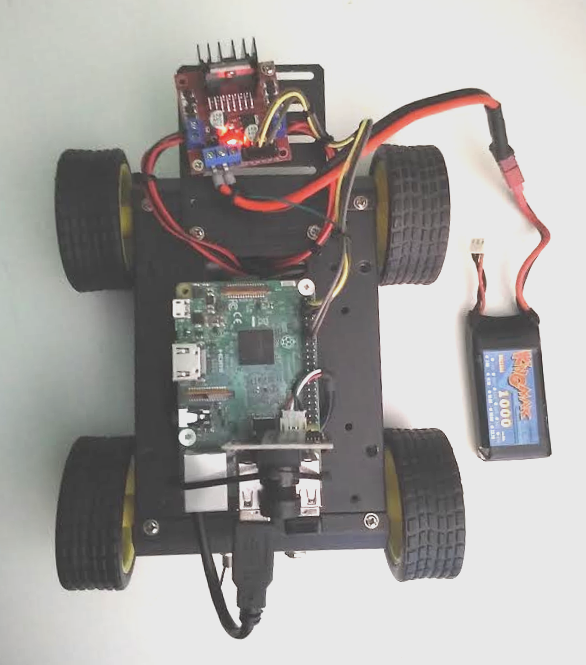
\includegraphics[scale=0.4]{imagenes/robot/robot-bateria-lipo.png}
  \end{center}
  \caption{Vista de la batería LiPo que alimenta los motores.}
  \label{figura:rpi-modulo-bateria}
\end{figure}



\subsubsection{Esquema de conexiones}

El siguiente gráfico \ref{diagrama:esquema-conexiones} muestra las conexiones de todo el conjunto:

\begin{figure}[H]
  \hspace*{.5in}{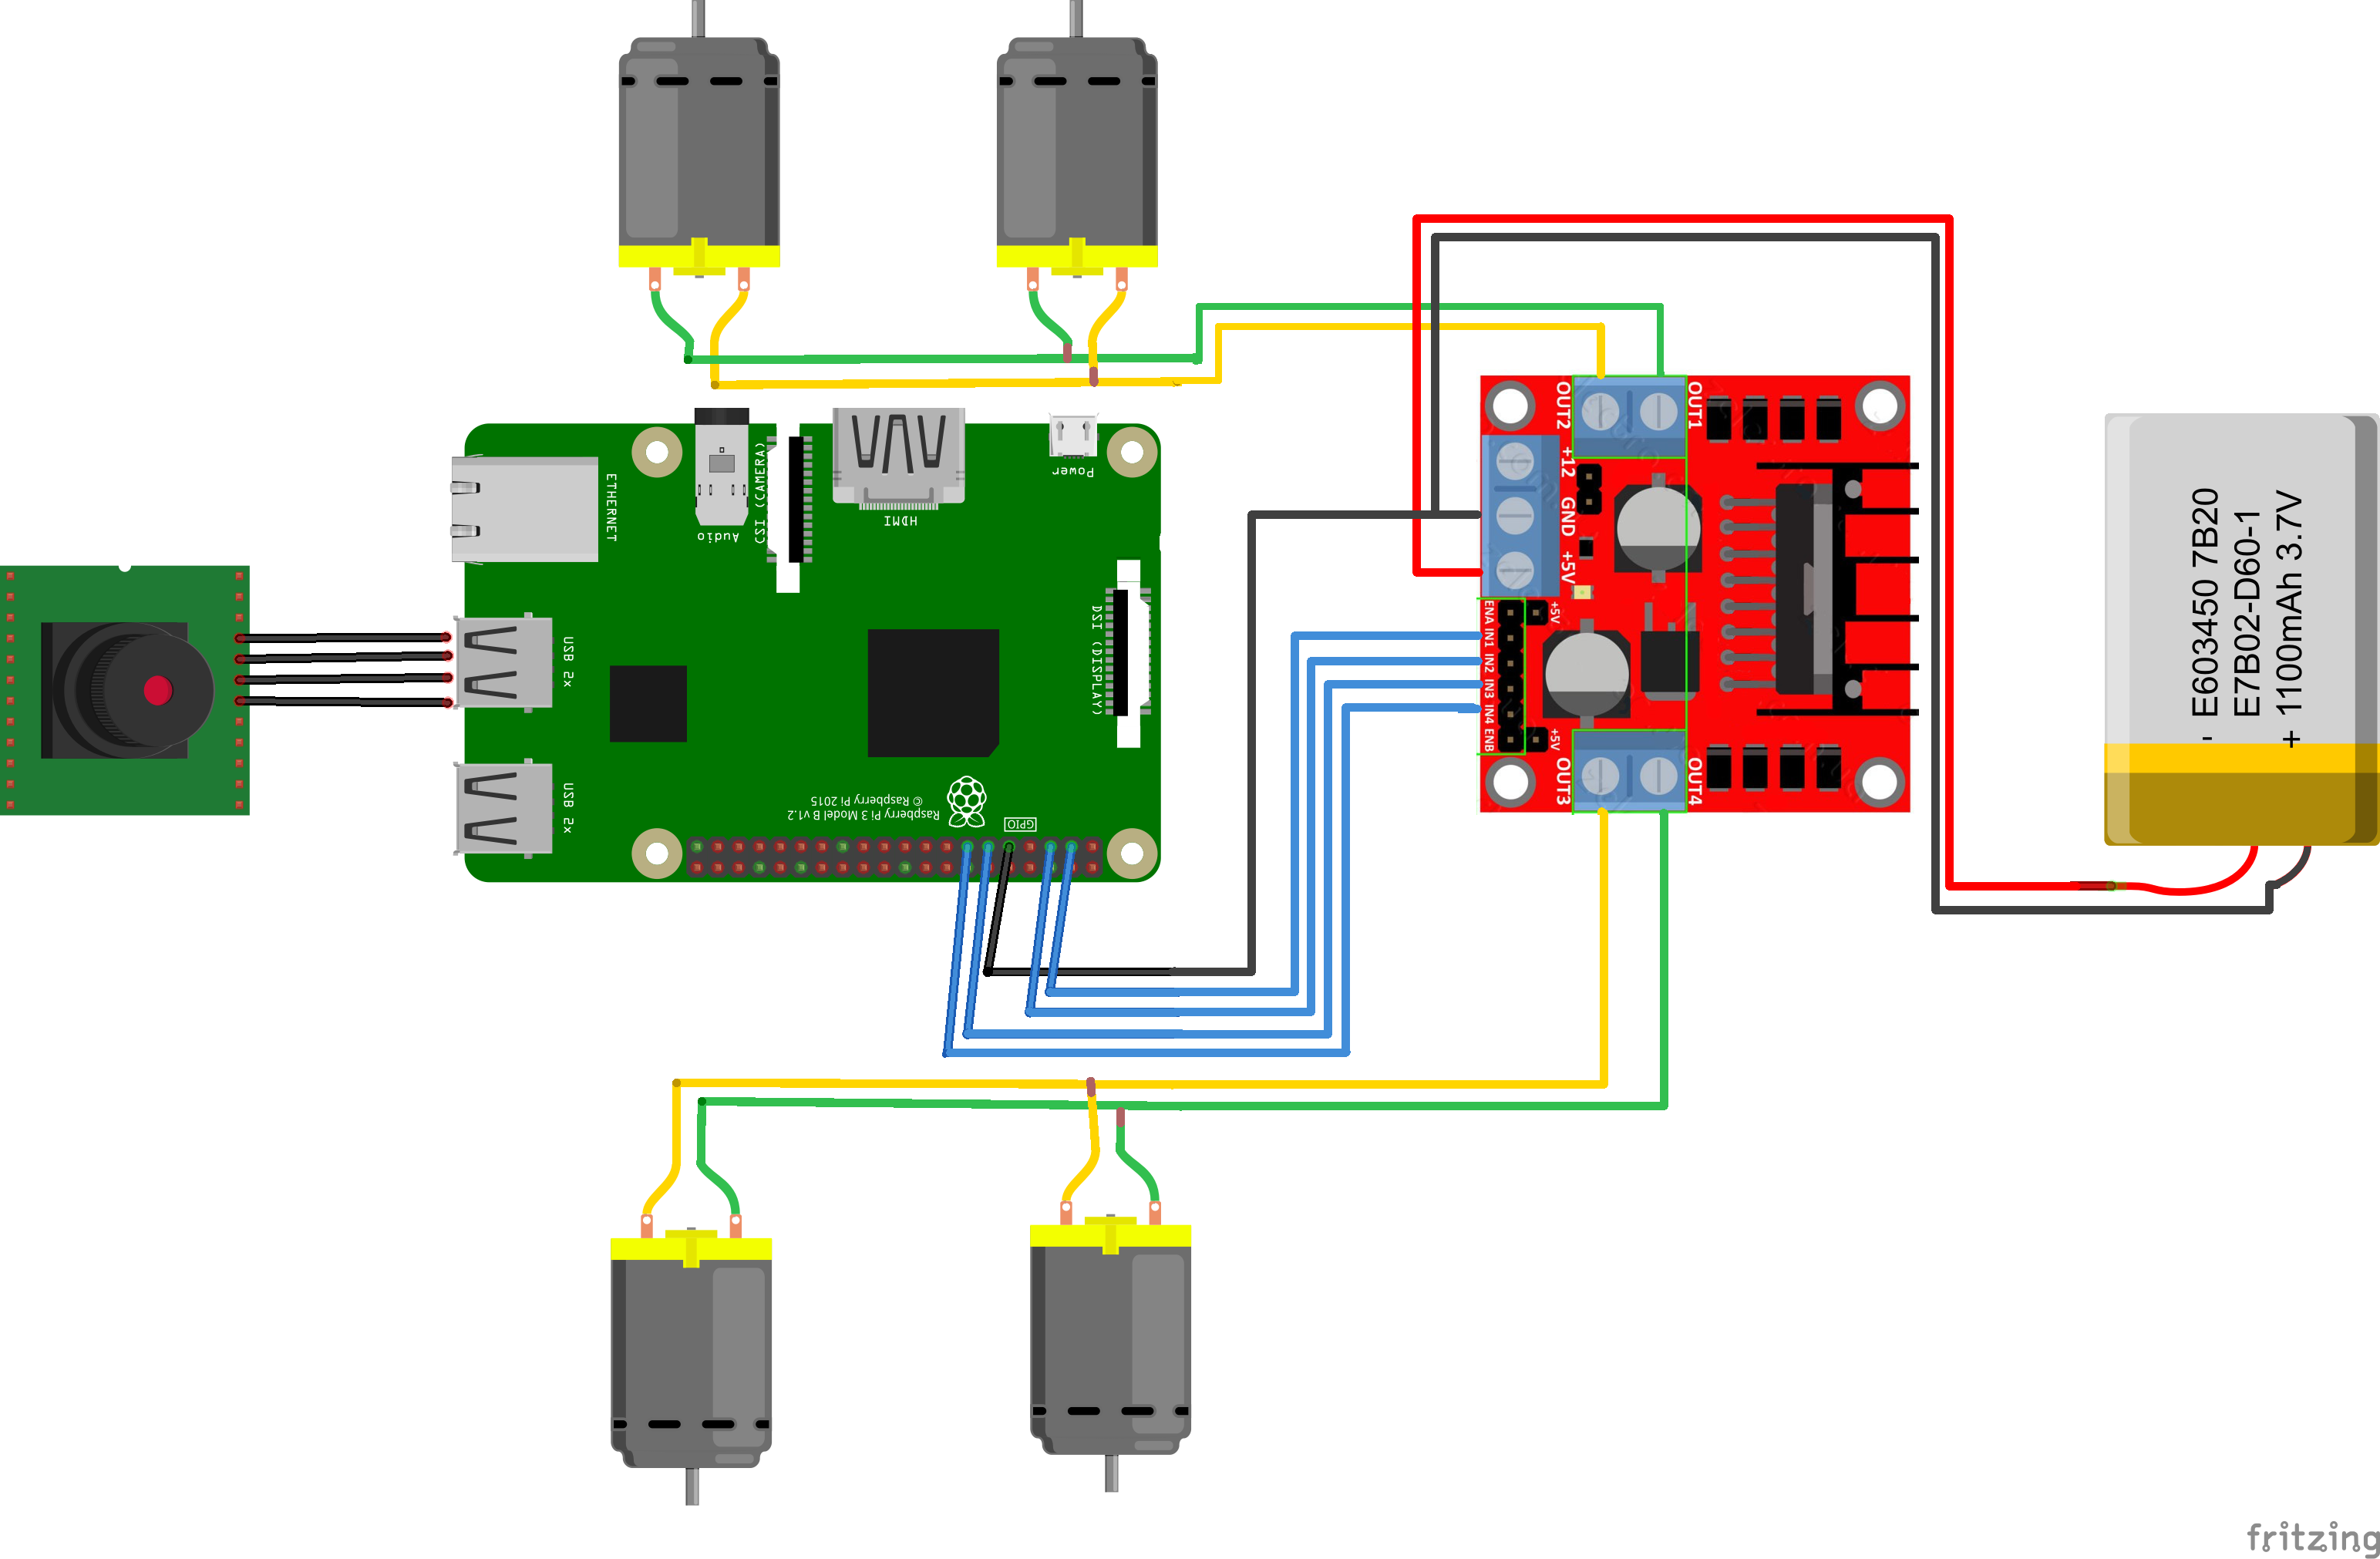
\includegraphics[scale=0.65,angle=270]{imagenes/robot/robot-esquema2.png}}
  \caption{Esquema de conexiones del robot de pruebas.}
  \label{diagrama:esquema-conexiones}
\end{figure}

    
\section{Software de control}
  

Para la programación del robot se ha empleado el lenguaje de programación JavaScript en un entorno de ejecución Node.js. A continuación se describirá aquellos aspectos más importantes
referentes al código desarrollado para el control del robot.\\

Primeramente se ha realizado la carga de librerías necesarias, entre ellas encontramos:

\begin{itemize}
 \item \emph{pigpio}: Módulo para la comunicación y control de los pines GPIO.
 \item \emph{child process}: El módulo child\_process proporciona la capacidad de generar procesos secundarios. Se ha empleado para la captura de vídeo mediante el lanzado de comandos ffmpeg.
 \item \emph{socket.io}: Biblioteca que establece enlaces bidireccionales en tiempo real y en comunicación basada por eventos.
\end{itemize}


\subsection{Entrada/Salida}

En segundo lugar se han definido los diferentes pines GPIO a utilizar y si serán empleados como pines de entrada o de salida:

\begin{table}[H]
  \begin{center}
    \begin{tabular}{|p{2.5cm}|p{2.5cm}|p{4.5cm}|}
      \hline
      {\textbf{GPIO}} & \textbf{ Modo } & \textbf{ Control }\\
      \hline
      {\textbf{ 2 }} & { OUTPUT } & { Motores lado izquierdo }  \\
     \hline
      {\textbf{ 3 }} & { OUTPUT } & { Motores lado izquierdo } \\
      \hline
      {\textbf{ 17 }} & { OUTPUT } & {  Motores lado derecho } \\
      \hline
      {\textbf{ 27 }} & { OUTPUT } & { Motores lado derecho } \\
     \hline   
    \end{tabular}
  \end{center}
\caption{ Configuración establecida para los puertos GPIO. }
\end{table}


Si para el vehículo que deseemos programar resultan necesarios más pines para la utilización de servos, sensores o cualquier otro elemento, tan solo debemos inicializarlos e indicar si van a ser pines de entrada
o de salida. Si existen dudas al respecto se puede acceder a la documentación de la biblioteca \emph{pigpio} en el siguiente enlace: \url{https://www.npmjs.com/package/pigpio}.
Para el caso de este proyecto, la inicialización de los pines se ha realizado mediante las siguientes instrucciones:

\begin{lstlisting}[language=JavaScript]
  // Carga del módulo.
  var Gpio = require('pigpio').Gpio;

  // Pines utilizados. Motores izquierdos: 2 y 3, motores derechos: 17 y 27
  var gpio2 = new Gpio(2, {mode: Gpio.OUTPUT}),
    gpio3 = new Gpio(3, {mode: Gpio.OUTPUT}),
    gpio17 = new Gpio(17, {mode: Gpio.OUTPUT}),
    gpio27 = new Gpio(27, {mode: Gpio.OUTPUT});
\end{lstlisting}


\subsection{Sockets}

Ahora bien, una vez definidos los pines que activarán nuestros motores necesitamos que éstos sean activados cuando desde una red externa lo indiquemos. Para ello emplearemos la biblioteca Socket.io. 
La cual debemos incluir en nuestro proyecto.

Para la creación del socket basta con la siguiente instrucción, la cual recibe un puerto que utilizará para mantenerse a la escucha: 

\begin{lstlisting}[language=JavaScript]
  var io = require('./node_modules/socket.io').listen(8085, { log: false });
\end{lstlisting}


Con la finalidad de ir capturando los diferentes eventos, se han definido las siguientes funciones para la conexión y desconexión de los clientes:

\begin{lstlisting}[language=JavaScript]

io.sockets.on('connection', function (socket)
{

  //Almacenamiento del número total de clientes conectados.
  sockets[socket.id] = socket;
  console.log("Total clientes conectados : ", Object.keys(sockets).length);
  
  //Envío de un saludo.
  socket.emit('robotmsg', {msg: "!!!HOLA!!!"});


  //Salida de un cliente.
  socket.on('disconnect', function() {
    console.log('Bye!');
    stopStreaming(socket);
  });  
  
}
\end{lstlisting}

Cuando un evento \emph{action} es recibido se activada la función que procesa el comando recibido y activa las salidas correspondientes, la cual establece los pines necesarios a los valores
1 o 0 según el parámetro establecido. La tabla \ref{table:table-pin-out} muestra las diferentes combinaciones de salidas y su acción correspondiente:

\begin{table}[H]
  \begin{center}
    \begin{tabular}{|p{2.5cm}|p{2.5cm}|p{2.5cm}|p{2.5cm}|p{2.5cm}|}
      \hline
      {\textbf{Acción}} & \textbf{ GPIO 2 } & \textbf{ GPIO 3 } & \textbf{  GPIO 17 } & \textbf{ GPIO 27 }\\
      \hline
      { \textbf{ UP } } & { 1 } & { 0 }  & { 1 }  & { 0 }  \\
      \hline
      { \textbf{ DOWN } } & { 0 } & { 1 }  & { 0 }  & { 1 } \\
      \hline
      { \textbf{ LEFT } } & { 1 } & { 0 }  & { 0 }  & { 0 } \\
      \hline
      { \textbf{ RIGHT } } & { 0 } & { 0 }  & { 1 }  & { 0 } \\
      \hline
      { \textbf{ STOP } } & { 0 } & { 0 }  & { 0 }  & { 0 }  \\
     \hline   
    \end{tabular}
  \end{center}
\caption{ Combinaciones de salida para los puertos GPIO y su acción correspondiente. }
\label{table:table-pin-out}
\end{table}

A continuación se muestra el ejemplo desarrollado para la activación de los motores en sentido de giro y dirección según la tabla anterior:\\

\begin{lstlisting}[language=JavaScript]
  // Escucha de comandos.  
  socket.on('action', function (data){

    console.log('Comando recibido: ' + data);

    switch(data) {
      case 'UP':
        gpio2.digitalWrite(1);
        gpio3.digitalWrite(0);
        gpio17.digitalWrite(1);
        gpio27.digitalWrite(0);
        console.log('UP');
        break;

      case 'RIGHT':
        gpio2.digitalWrite(0);
        gpio3.digitalWrite(0);
        gpio17.digitalWrite(1);
        gpio27.digitalWrite(0);
        console.log('UP');
        break;

      case 'LEFT':
        gpio2.digitalWrite(1);
        gpio3.digitalWrite(0);
        gpio17.digitalWrite(0);
        gpio27.digitalWrite(0);
        console.log('UP');
        break;

      case 'DOWN':
        gpio2.digitalWrite(0);
        gpio3.digitalWrite(1);
        gpio17.digitalWrite(0);
        gpio27.digitalWrite(1);
        console.log('UP');
        break;

      case 'STOP':
        gpio2.digitalWrite(0);
        gpio3.digitalWrite(0);
        gpio17.digitalWrite(0);
        gpio27.digitalWrite(0);
        console.log('UP');
        break;

      default:
        console.log('command not found');
    }

  })
    
\end{lstlisting}



\subsection{ Streaming de vídeo }

Para realizar la transferencia de vídeo desde el robot hacia el cliente se ha realizado empleado las librerías FFmpeg haciendo uso de su herramienta de línea de comandos.\\

El procedimiento de captura de vídeo y su posterior transmisión es realizado mediante la siguiente instrucción de Ffmpeg:\\

\begin{lstlisting}[language=bash]
  ffmpeg -f video4linux2 -i /dev/video0 -s 300x150 -f mjpeg pipe:1 -b:v 28k -bufsize 28k
\end{lstlisting}

En los puntos sucesivos analizaremos qué es lo que realiza la instrucción anterior y por qué resulta clave en todo el proceso de difusión, comprendido desde la captura del 
vídeo hasta su posterior transmisión al usuario que está controlando el robot.\\

Nada prodríamos transmitir si no disponemos inicialmente de los datos que queremos difundir. De ahí que inicialmente debamos realizar la captura de las diferentes imágenes a partir de la cámara
USB conectada a la Raspberry Pi. Para ello se utiliza la API de captura de vídeo video4linux2 \footnote{ Video4Linux o V4L es una API de captura de video para Linux. Muchas webcams USB, sintonizadoras
de tv, y otros periféricos son soportados. Video4Linux está integrado con el núcleo Linux. V4L está en su segunda versión (V4L2). El V4L original fue incluido en el ciclo 2.1.X de desarrollo del
núcleo Linux. Video4Linux2 arregla algunos fallos y apareció en los núcleos 2.5.X. } (o simplemente v4l2) la cual dispone las bibliotecas de Ffmpeg. Tan solo debemos especificar el dispositivo de 
captura.\\

El nombre del dispositivo de captura es un nodo de dispositivo de archivo, por lo general los sistemas Linux tienden a crear automáticamente estos nodos cuando el dispositivo
está conectado al sistema, y ​​tiene un nombre del tipo /dev/videoN, donde N es un número asociado al dispositivo.\\ 


Para proceder a la captura de las imágenes nos bastaría con introducir el siguiente comando:

\begin{lstlisting}[language=bash]
  ffmpeg -f video4linux2 -i /dev/video0 -s 300x150 -f mjpeg video_out.mpeg
\end{lstlisting}

Ahora bien, el comando anterior toma las imágenes de la cámara y las almacena en el archivo especificado \emph{ video\_out.mpeg} especificando una resolución de salida de 300x150 píxeles
empleando la opción -s. Pero nosotros no deseamos exactamente ese comportamiento. Debemos canalizar esos datos capturados hacia el socket creado con la finalidad de ir transmitiendo los 
diferentes frames y no almacenándolos en disco tal y como realiza la instrucción anterior.\\


Para resolver este problema podemos emplear el sistema de tuberías que implementan los sistemas UNIX \footnote{ Una tubería (pipe, cauce o '|') consiste en una cadena de 
procesos conectados de forma tal que la salida de cada elemento de la cadena es la entrada del próximo. Permiten la comunicación y sincronización entre procesos. Es común el uso de
buffer de datos entre elementos consecutivos. }.

En cualquier sistema Unix se puede hacer que la salida de una determinada orden sea la entrada estándar de otra, lo que le confiere a las órdenes Unix una enorme potencia.
Para realizar dicha "canalización`` debemos utilizar las siguientes opciones:\\

\begin{lstlisting}[language=bash]
  pipe:1 -b:v 28k -bufsize 28k
\end{lstlisting}


Con la opción \emph{pipe:1} accedemos al protocolo pipe de UNIX, el cual lee y escribe de las \emph{tuberias} UNIX siendo el número 1 la tubería correspondiente a la salida estándar 
stdout ( 0 para stdin y 2 para stderr), la cual podría ser omitida puesto que es la salida por defecto.\\

La opción \emph{-b:v 28k} establece la tasa de transferencia, en nuestro caso una tasa de 28 kbit/s.\\

La opción \emph{-bufsize 28k} establece un tamaño de buffer \footnote{Un buffer de datos es un espacio de la memoria en un disco o en un instrumento digital reservado para el almacenamiento
temporal de información digital, mientras que está esperando ser procesada.} de 28 kbits.\\

A continuación mostramos el código de transmisión de vídeo al completo junto con la captura de los diferentes eventos cuando se producen salida de datos por cada una de las salidas estándar:\\

\begin{lstlisting}[language=JavaScript]

  function startStreaming(socket) {
    //ffmpeg -f video4linux2 -i /dev/video0 -s 300x150 -f mjpeg pipe:1 -b:v 28k -bufsize 28k

    if (running_camera == false){
      console.log('Starting streaming....');
      var args = ["-f", "video4linux2", "-i", "/dev/video0", "-s", "300x150","-f","mjpeg", "pipe:1", "-b:v 28k", "-bufsize 28k"]
      ffmpeg_command = require('child_process').spawn("ffmpeg", args);
      running_camera = true
    }

    ffmpeg_command.on('error', function(err, stdout, stderr) {
      console.log("ffmpeg stdout:\n" + stdout);
      console.log("ffmpeg stderr:\n" + stderr);
      running_camera = false
    });


    ffmpeg_command.on('close', function (code) {
      console.log('ffmpeg exited' + code );
      running_camera = false
    });


    ffmpeg_command.stderr.on('data', function (data) {
      //console.log('stderr: ' + data);
    });

    ffmpeg_command.on('end', function() {
      console.log('Finished');
      running_camera = false
    });

    ffmpeg_command.stdout.on('data', function (data) {
      //console.log('stdout: ' + data);
      var frame = new Buffer(data).toString('base64');
      socket.emit('canvas',frame);
    });
  }

\end{lstlisting}



\subsection{Código de ejemplo completo}

Finalmente se muestra el código completo para el robot de pruebas desarrollado. Dicho código puede emplearse como guía de referencia para futuros proyectos con la idea de integrarlos en la aplicación RobotUI.\\


\begin{lstlisting}[language=JavaScript]
// Inicia servidor socket.io en el puerto 8085.
var io = require('./node_modules/socket.io').listen(8085, { log: false });

// Carga de módulos necesarios.
var ffmpeg_command, running_camera = false, Gpio = require('pigpio').Gpio, child_process = require('child_process');

// Pines utilizados. Motores izquierdos: 2 y 3, motores derechos: 17 y 27
var gpio2 = new Gpio(2, {mode: Gpio.OUTPUT}),
  gpio3 = new Gpio(3, {mode: Gpio.OUTPUT}),
  gpio17 = new Gpio(17, {mode: Gpio.OUTPUT}),
  gpio27 = new Gpio(27, {mode: Gpio.OUTPUT});


console.log('Esperando conexión...');

var sockets = {};

io.sockets.on('connection', function (socket)
{

  sockets[socket.id] = socket;
  console.log("Clientes totales conectados: ", Object.keys(sockets).length);

  socket.on('disconnect', function() {
    console.log('¡Adios!');
    //stopStreaming(socket);
  });


  socket.on('start-stream', function() {
    startStreaming(socket);
  });

  socket.emit('robotmsg', {msg: "¡¡¡Bienvenido!!!"});
  console.log('emitiendo: ' + "¡¡¡Bienvenido!!!");

  socket.on('action', function (data){

    console.log('Comando recibido: ' + data);

    switch(data) {
      case 'UP':
        gpio2.digitalWrite(1);
        gpio3.digitalWrite(0);
        gpio17.digitalWrite(1);
        gpio27.digitalWrite(0);
        console.log('UP');
        break;

      case 'RIGHT':
        gpio2.digitalWrite(0);
        gpio3.digitalWrite(0);
        gpio17.digitalWrite(1);
        gpio27.digitalWrite(0);
        console.log('UP');
        break;

      case 'LEFT':
        gpio2.digitalWrite(1);
        gpio3.digitalWrite(0);
        gpio17.digitalWrite(0);
        gpio27.digitalWrite(0);
        console.log('UP');
        break;

      case 'DOWN':
        gpio2.digitalWrite(0);
        gpio3.digitalWrite(1);
        gpio17.digitalWrite(0);
        gpio27.digitalWrite(1);
        console.log('UP');
        break;

      case 'STOP':
        gpio2.digitalWrite(0);
        gpio3.digitalWrite(0);
        gpio17.digitalWrite(0);
        gpio27.digitalWrite(0);
        console.log('UP');
        break;

      default:
        console.log('command not found');
    }

  })
});

function stopStreaming(socket) {
  delete sockets[socket.id];
  // no more sockets, kill the stream
  if (Object.keys(sockets).length == 0) {
    if (ffmpeg_command){
      ffmpeg_command.kill();
      running_camera = false;
      console.log('Stop streaming');
    }
  }
}

function startStreaming(socket) {
  //ffmpeg -f video4linux2 -i /dev/video0 -s 300x150 -f mjpeg pipe:1 -b:v 28k -bufsize 28k

  if (running_camera == false){
    console.log('Starting streaming....');
    var args = ["-f", "video4linux2", "-i", "/dev/video0", "-s", "300x150","-f","mjpeg", "pipe:1", "-b:v 28k", "-bufsize 28k"]
    ffmpeg_command = child_process.spawn("ffmpeg", args);
    running_camera = true
  }

  ffmpeg_command.on('error', function(err, stdout, stderr) {
    console.log("ffmpeg stdout:\n" + stdout);
    console.log("ffmpeg stderr:\n" + stderr);
    running_camera = false
  });


  ffmpeg_command.on('close', function (code) {
    console.log('ffmpeg exited' + code );
    running_camera = false
  });


  ffmpeg_command.stderr.on('data', function (data) {
    //console.log('stderr: ' + data);
  });

  ffmpeg_command.on('end', function() {
    console.log('Fin');
    running_camera = false
  });

  ffmpeg_command.stdout.on('data', function (data) {
    //console.log('stdout: ' + data);
    var frame = new Buffer(data).toString('base64');
    socket.emit('canvas',frame);
  });

}

\end{lstlisting}


Para la ejecución del código introducimos el siguiente comando:

\begin{lstlisting}[language=bash]
  sudo node raspberry.js
\end{lstlisting}

Siendo \emph{raspberry.js} el nombre del archivo que contiene nuestro código.


\chapter{Organización temporal}
\label{chap:planificación}

La planificación general del proyecto siguiendo un modelo SCRUM, empleando para ello el panel de tareas Trello; un gestor de proyectos que permite aplicar una metodología de desarrollo ágil.\\

El panel se encuentra accesible en el siguiente enlace: \url{https://trello.com/b/SpIbFI7k/robotui}.

\begin{figure}[H]
\hspace*{-.2in}{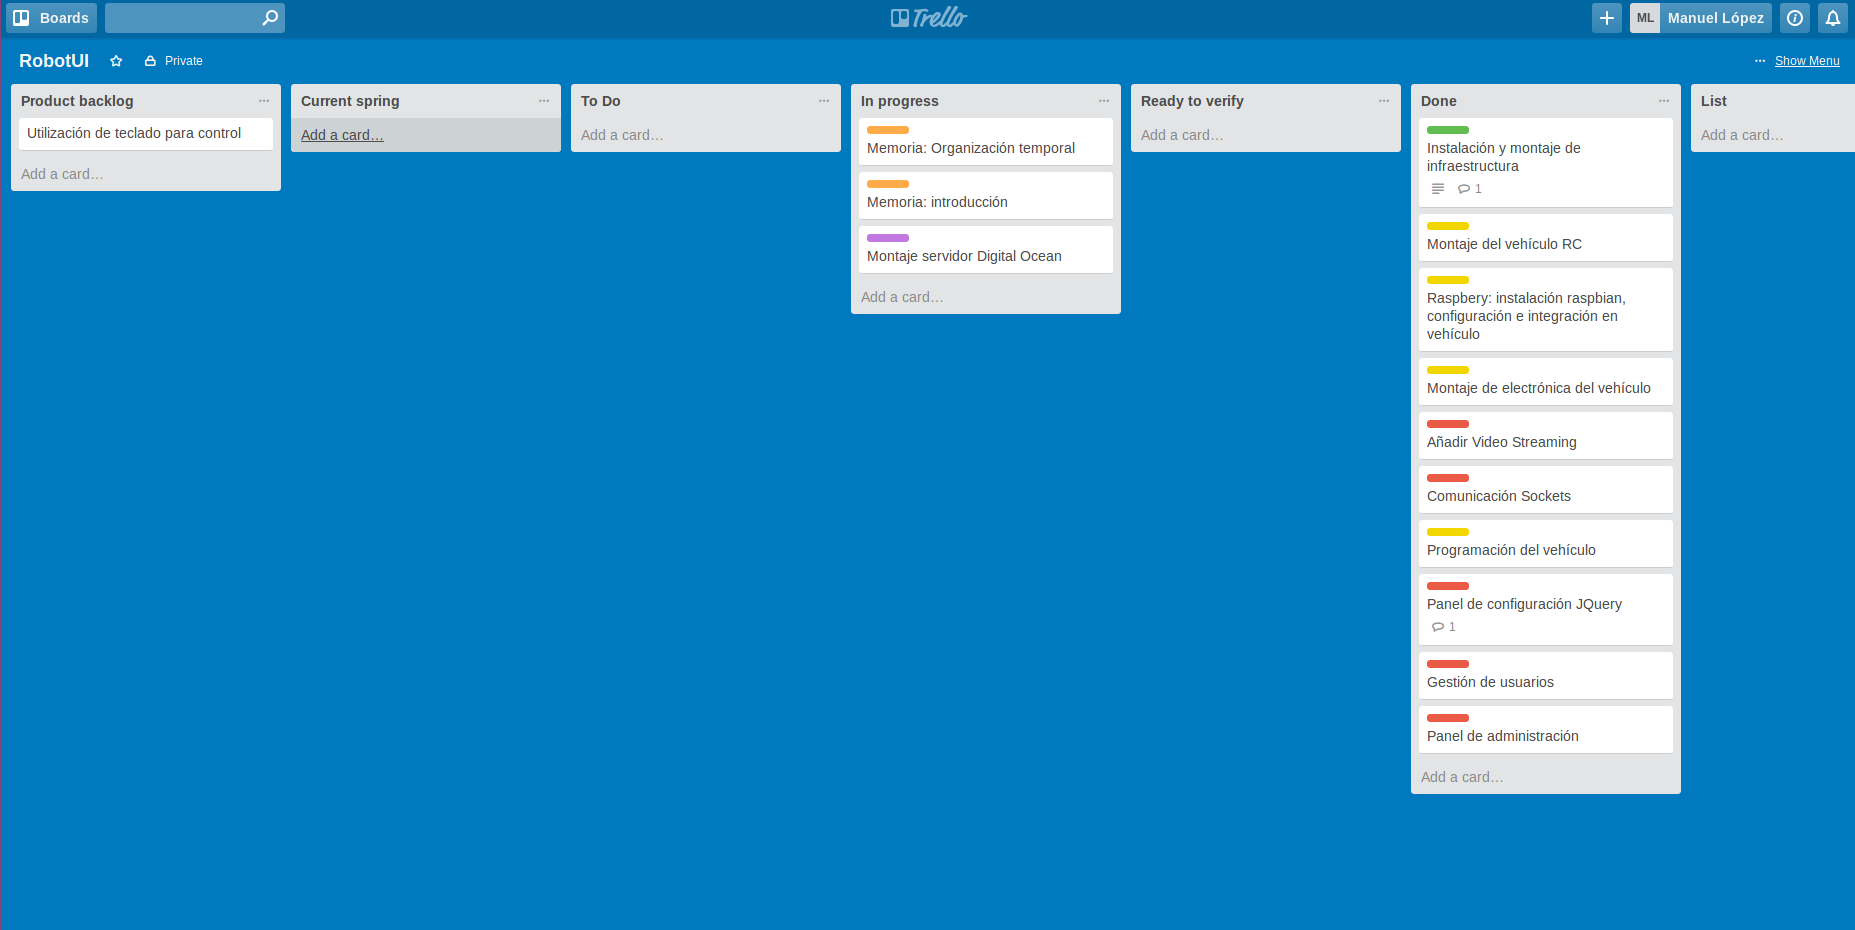
\includegraphics[scale=0.25]{imagenes/panel-trello.png}}
\caption{Panel de actividades - Trello}
\end{figure}


Cabe destacar que para el desarrollo de RobotUI ha sido necesario emplear varias herramientas, utilidades y bibliotecas. Algunas de ellas ya habían sido utilizadas en ciertas ocasiones, bien sea en el ámbito estudiantil o profesional. 
Sin embargo, otras han requerido un periodo de formación previo, en el que se han adquirido los conocimientos necesarios para poder desarrollar el presente proyecto.\\

La mayor parte del proceso de investigación fue dedicado al estudio de las diferentes tecnologías existentes para la programación web en tiempo real. Todo ello ha implicado un esfuerzo bastante considerable en el uso, 
aprendizaje e investigación de las diferentes tecnologías existentes y comprobar su potencial.\\

Una vez determinadas las diferentes herramientas a utilizar se comenzó con la implementación de la aplicación, siendo seleccionada como herramienta principal el framework Sails.js. Un framework MVC en 
tiempo real para Node.js, el cual está muy enfocado al propósito de este proyecto.\\

Finalmente, tras la necesidad de probar la aplicación en un entorno real, se optó por elaborar un robot de pruebas, un pequeño vehículo elaborado con una Raspberry Pi con la finalidad de probar, testear y hacer 
demostraciones de la aplicación.

La figura \ref{gantt:tareas01} y \ref{gantt:tareas02} muestran una visión de las diferentes tareas desarrolladas para la elaboración del proyecto junto con la descomposición de cada una de ellas:\\

\begin{figure}
  \begin{center}
    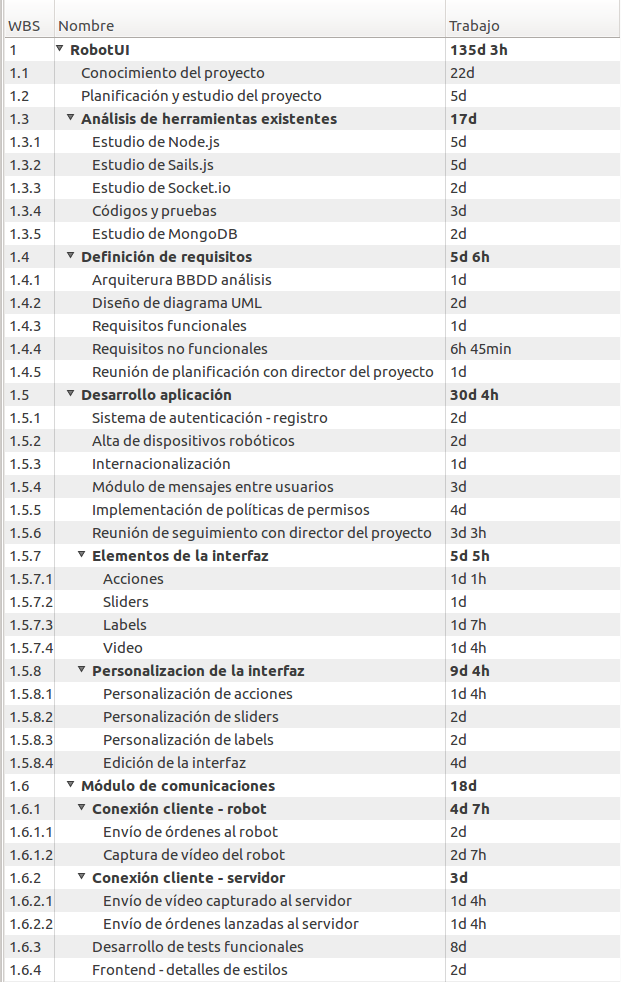
\includegraphics[scale=0.6]{imagenes/planificacion/descomposicion_tareas01.png}
  \end{center}
  \caption{Descomposición de las tareas implicadas en el desarrollo del proyecto (Primera Parte).}
  \label{gantt:tareas01}
\end{figure}


\begin{figure}
  \begin{center}
    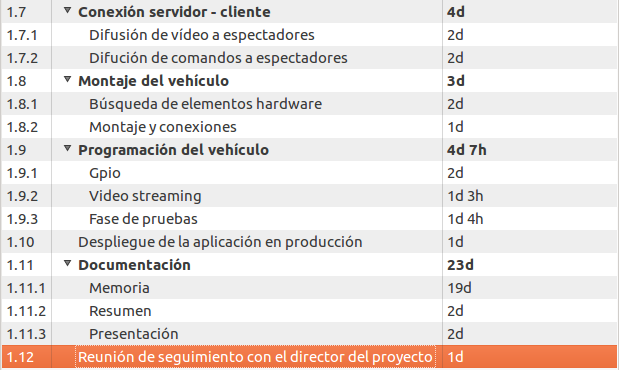
\includegraphics[scale=0.6]{imagenes/planificacion/descomposicion_tareas02.png}
  \end{center}
  \caption{Descomposición de las tareas implicadas en el desarrollo del proyecto (Segunda parte).}
  \label{gantt:tareas02}
\end{figure}

Los puntos más importantes del proyecto se han dividido en hitos, así como entregas que se definieron en cada reunión que se realizaba con el director del proyecto. 
También se ha definido una planificación temporal del desarrollo del proyecto mediante un diagrama de Gantt con la duración de las tareas recogidas en el panel de actividades de Trello.\\
\newpage


\section{Planificación temporal de tareas}

A continuación se definirán los diferentes hitos que componen el diagrama de Gantt divididos en las diferentes subtareas principales de cada uno de ellos:\\

\subsection{Hito 1: Planificación y análisis }
\label{subsec:hito1}

En esta primera etapa de desarrollo del proyecto final de carrera se realizaron los estudios previos necesarios para abordar cualquier proyecto de cierta envergadura.

Este hito se descompone en las siguientes tareas principales:

\begin{enumerate}
 \item Planificación y estudio del proyecto. En esta fase se centró en la elaboración de un documento, a modo borrador, con la idea a desarrollar, objetivos del proyecto y su alcance.
 \item Análisis de herramientas existentes, de las tecnologías a implementar, la arquitectura del sistema, las tecnologías de BD, visualización, para la selección de las herramientas más adecuadas 
 para afrontar el desarrollo con garantías y no sea necesaria una ``vuelta atrás'' por necesidad imperiosa de cambio de tecnología. En definitiva se buscaba una herramienta libre, con un respaldo de una comunidad importante
 y que resuelva la problemática o necesidad de trabajar con eventos en tiempo real.
\end{itemize}

\subsection{Hito 2: Definición de requisitos }
\label{subsec:hito2}

Este segundo hito queda dividido en las siguientes etapas:

\begin{enumerate}
 \item Elaboración de un documento formal con la propuesta de proyecto definiendo sus objetivos y alcance, para la aprobación por parte del director del proyecto.
 \item Se definen las clases del sistema, el modelo de la base de datos y la definición de requisitos funcionales y no funcionales. 
\end{enumerate}

\subsection{Hito 3: Comienzo de desarrollo de la aplicación}
\label{subsec:hito3}

En este tercer hito, uno de los de mayor magnitud, se comienza con el desarrollo de la aplicación, el cual queda dividido en las siguientes módulos.

\begin{enumerate}
 \item Implementación del módulo \emph{Usuario} con las funciones de registro, autenticación, configuraciones de idioma, entre otras.
 \item Implementación del módulo central de la aplicación \emph{Robot}
 \item Implementación del módulo de mensajes.
 \item Implementación del módulo de políticas de permisos.
\end{enumerate}


\subsection{ Hito 4: Desarrollo de la aplicación, módulo componentes }
\label{subsec:hito4}

En este hito, se trabaja en el desarrollo de los diferentes elementos que compondrán la interfaz de control. Tanto su parte de configuración y personalización. 
Cada elemento integrante de la interfaz lo denominamos componentes.\\

En definitiva, el hito queda dividido en el desarrollo de los siguientes componentes:

\begin{enumerate}
 \item \emph{Acciones}
 \item \emph{Sliders}
 \item \emph{Labels}
 \item \emph{Vídeo}
\end{enumerate}


\subsection{Hito 5: Desarrollo de la aplicación, módulo interfaz }
\label{subsec:hito5}

En este hito, se realiza la elaboración de la interfaz de control. Tanto su parte de configuración y personalización como la de visualización para su control. Este hito quedó dividido 
en las siguientes etapas:

\begin{enumerate}
 \item Impementación de la funcionalidad de configuración
 \item Implementación de la funcionalidad de control
\end{enumerate}


\subsection{Hito 6: Desarrollo del módulo de comunicaciones }
\label{subsec:hito6}

El presente hito, clasificado como crítico debido a su importancia. Debía realizar la integración de todos los módulos anteriores y dotarlos de la funcionalidad principal para la que han sido diseñados. Estar interconectados 
entre sí además de la elaboración de los test funcionales.

\begin{enumerate}
 \item Impementación de la conexión cliente - robot.
 \item Implementación de la conexión cliente - servidor.
 \item Desarrollo de test funcionales.
\end{enumerate}


\subsection{Hito 7: Construcción del vehículo de pruebas }
\label{subsec:hito6}

Se realiza la construcción y montaje e instalación software del vehículo de pruebas y comprobación de las diferentes conexiones.

\subsection{Hito 8: Programación del vehículo de pruebas }
\label{subsec:hito6}

Se realiza la programación del vehículo y se realizan pruebas de todo el conjunto junto con las correcciones necesarias.


\subsection{Hito 9: Documentación }
\label{subsec:hito6}

Se finaliza la memoria para la revisión por parte del director del proyecto y su posterior impresión. Se prepara la presentación para la defensa ante tribunal.


\section{Diagrama de Gantt}

A continuación se muestra el diagrama de Gantt donde quedan reflejados los diferentes hitos descritos en el punto anterior.

\begin{figure}
  \hspace*{.8in}{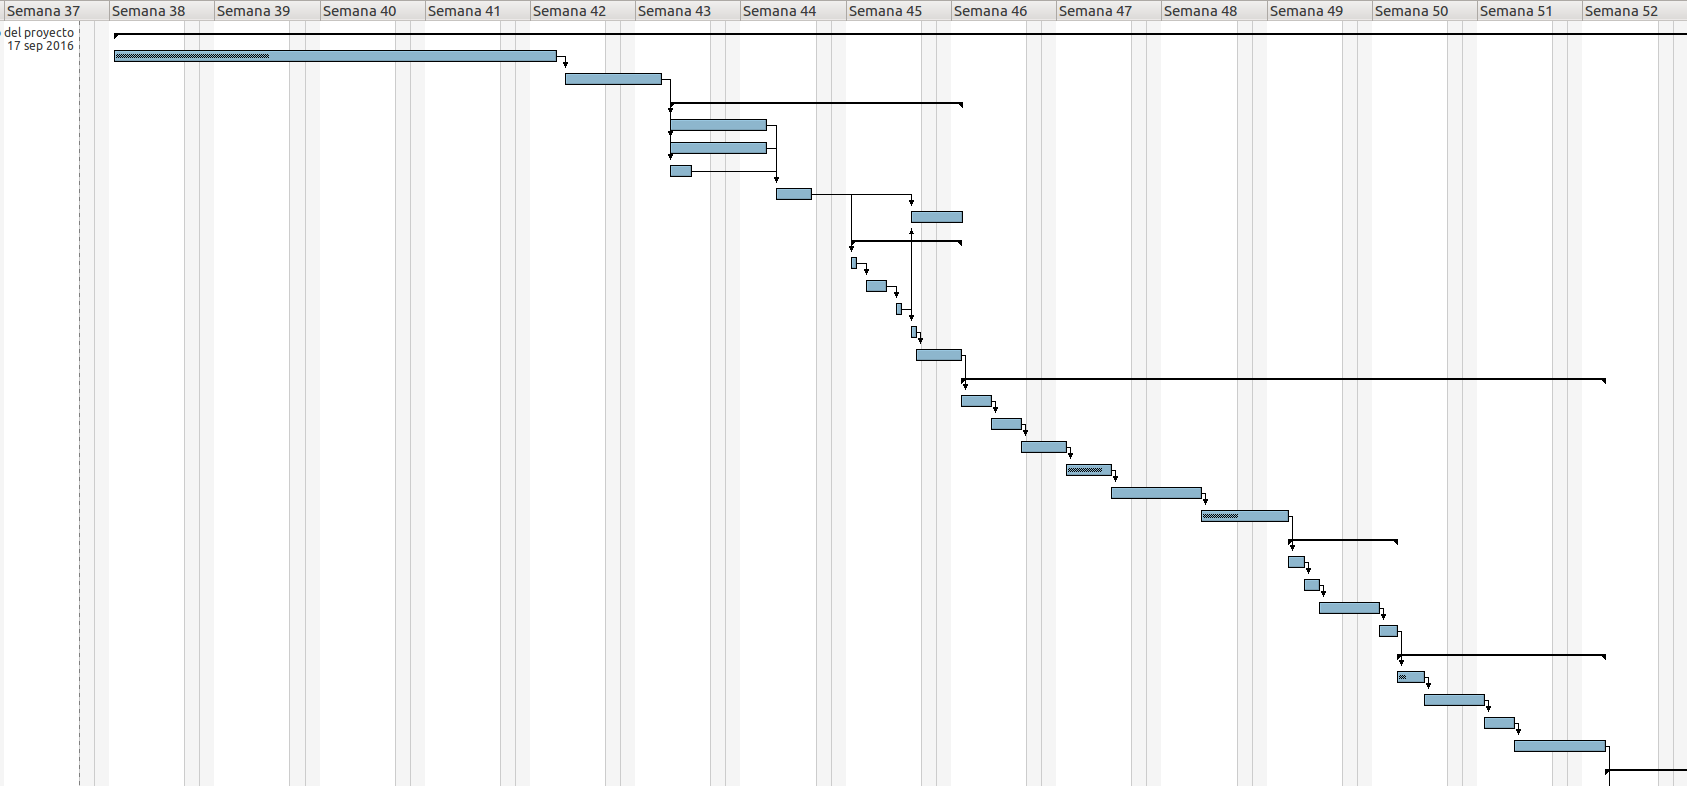
\includegraphics[scale=0.38,angle=270]{imagenes/planificacion/gantt01.png}}
  \caption{Diagrama de Gantt 1. Desarrollo del proyecto.}
\end{figure}

\begin{figure}
  \hspace*{.8in}{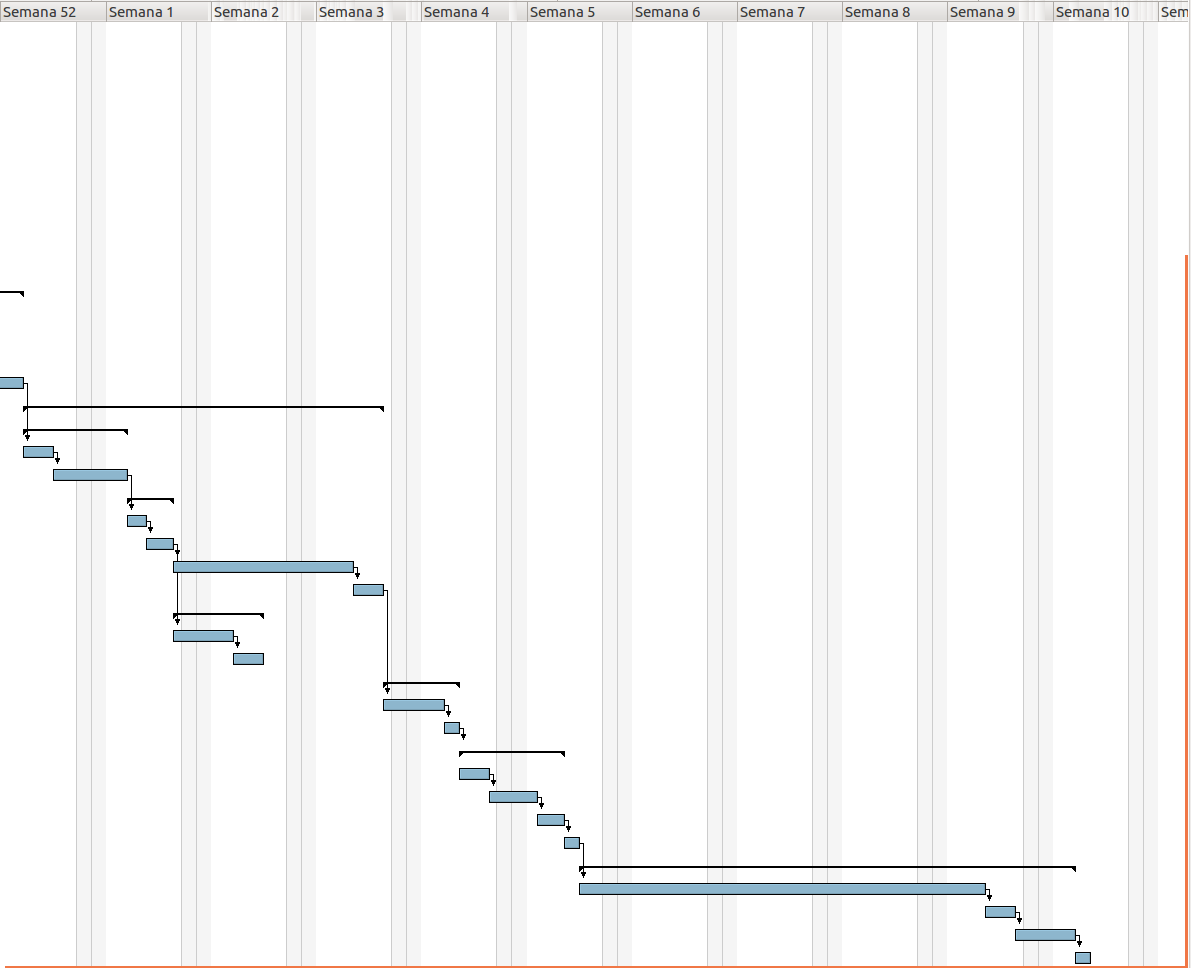
\includegraphics[scale=0.38,angle=270]{imagenes/planificacion/gantt02.png}}
  \caption{Diagrama de Gantt 2. Desarrollo del proyecto.}
\end{figure}

\newpage


\chapter{ Guía de Usuario}
\label{chap:manual-usuario}

La aplicación RobotUI ha sido creada por Manuel López Urbina para el proyecto fin de carrera de la titulación de Ingeniería Informática de la Universidad de Cádiz.\\

Resulta de vital importancia consultar esta guía antes y/o durante la utilización de los diferentes elementos tanto hardware, robot de pruebas desarrollado, como software del presente proyecto ya 
que le proporcionará una guía paso a paso en el manejo correcto de la aplicación.\\

La resolución recomendada para la aplicación debe ser superior o igual a 1024x768 (Estándar XGA), aunque es adaptable a cualquier resolución debido a su diseño web responsive.\\

RobotUI ha sido elaborado con un claro propósito; el de  proporcionar a los usuarios un medio donde compartir sus dispositivos robóticos con el resto de usuarios. Esto es posible gracias a una serie de
herramientas desarrolladas para que, sin necesidad de tener grandes conocimientos en programación, puedan configurar un entorno para el manejo de sus proyectos robóticos y tener 
posibilidad de compartir sus dispositivos y experiencias con el resto de usuarios.\\

La particularidad de RobotUI es que el usuario propietario del robot tiene la posibilidad de permitir el manejo de sus dispositivos robóticos al resto de usuarios que él mismo considere de una 
manera controlada o, por otra parte, permitir que otros usuarios visualicen, como si de espectadores se tratase, el control que un determinado usuario realiza de un determinado robot.
Todo ello en tiempo real.\\

Por tanto, tras esta breve introducción en el ámbito de la aplicación, en este manual se describen los diferentes pasos a realizar para configurar sus dispositivos correctamente en el sistema
y abrirlo a toda una comunidad de usuarios. Además de tener abierto el acceso a otros muchos dispositivos de otras personas.\\

\subsection{Objetivo de esta guía}

Esta guía tiene como objetivo proporcionar al usuario un soporte de ayuda e iniciación a la utilización de RobotUI.\\

Esta sección comprende:\\

\begin{itemize}
 \item Introducción.
 \item Guía de acceso al código fuente de la aplicación.
 \item Guía de uso de la aplicación.
 \item Guía para la puesta en marcha y programación de un robot.
\end{itemize}

\subsection{Dirigido a}

Esta guía esta dirigida al usuario final del proyecto SensorRS. Tiene la finalidad de proporcionar una guía descriptiva de los procedimientos de creación, configuración y utilización de los diferentes dispositivos 
robóticos en sus dos modalidades disponibles, la de control y la de visualización.

\subsection{Obtener SensorRS}

El código fuente junto con la presente memoria se encuentra disponible en el repositorio GitHub en el enlace \url{https://github.com/lopomaster/SensorRS} o usando la herramienta
Git, escribiendo en la consola el siguiente comando:\\

\begin{lstlisting}[language=bash]
 git clone git@github.com:lopomaster/SensorRS.git 
\end{lstlisting}


\section{ Uso de SensorRS }
\label{sec:uso-sensorrs}


\subsection{ Configuración }
\label{sec:configuracion}

Para la puesta en funcionamiento es necesario establecer una series de configuraciones en el código del robot con la finalidad de conectarlo a la aplicación RobotUI.\\

El manual de usuario de RobotUI se encuentra accesible en el respositorio del proyecto localizado en \url{ https://github.com/lopomaster/SAILS-RobotUI }
Para acceder a la aplicación, el usuario deberá acceder al siguiente enlace: \url{www.robotui.com}. \\

Al acceder podrá ver el portal de entrada a la aplicación. En él puede acceder al resto de funcionalidades identificándose con sus credenciales y acceder a los formularios de registro
de usuario.\\

\begin{figure}[H]
  \begin{center}
    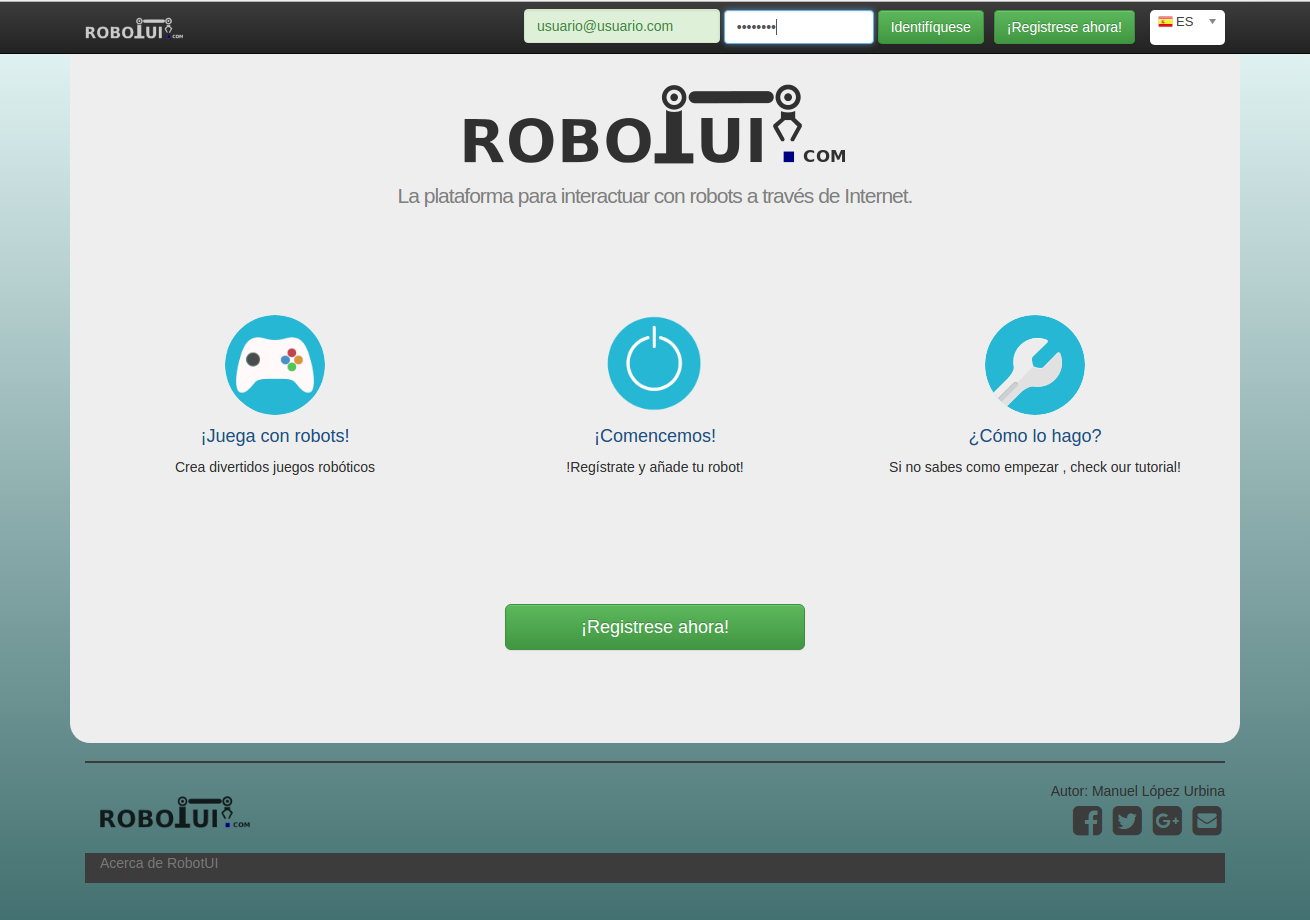
\includegraphics[scale=0.3]{imagenes/manual-usuario/pagina-principal.png}
  \end{center}
  \caption{Página principal RobotUI.}
  \label{website:pagina-principal}
\end{figure}


\subsection{ Programa tu robot }
\label{sec:programacion-robot}

NOTA: Esta guía comprende una serie de pasos para realizar la programación de un dispositivo robótico para la aplicación RobotUI. En este caso particular, el robot empleado posee como base una placa 
Raspberry Pi, la cual emplea para la conexión de sensores y motores haciendo uso de su sistema de Entrada/Salida Gpio.\\

El sistema es compatible con cualquier dispositivo, no solo limitado a las placas Raspberry. La única diferencia radica en que se deberán emplear a nivel de programación las bibliotecas adecuadas 
para la activación o lectura de las Entadas/Salidas correspondientes al modelo de placa utilizado.\\

Antes de proceder con la programación de nuestro robot debemos de realizar su creación en la aplicación RobotUI como queda descrito en el punto \ref{sec:creacion-robot} y 
tomar nota del identificador único que la aplicación proporciona para dicho robot y que posteriormente necesitaremos.\\	

\begin{figure}[H]
  \begin{center}
    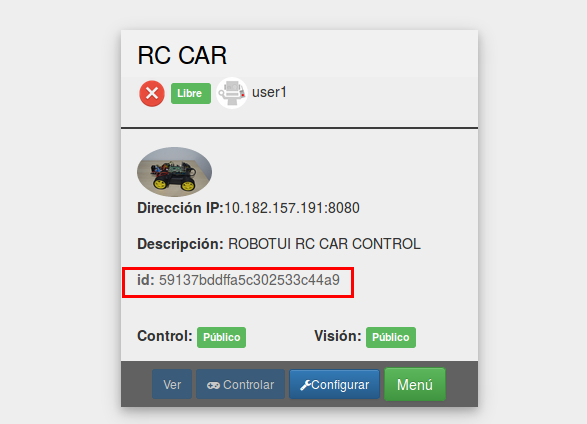
\includegraphics[scale=.6]{imagenes/manual-usuario/identificador.png}
  \end{center}
  \caption{Panel informativo de un robot donde se aprecia su identificador.}
  \label{website:pagina-principal}
\end{figure}

Una vez creado el robot y configurada su interfaz, añadiendo los diferentes elementos disponibles como acciones, vídeo, etiquetas, etcétera, recogidos en el punto \ref{subsec:configuracion-interfaz}: Configuración de la interfaz.
Podemos comenzar con la programación del robot.\\

Para ello debemos seguir una serie de pasos:\\

\begin{enumerate}
  \item Generar una archivo de extensión .js, con el código base mostrado en el punto \ref{codigo:base}.
  \item Reemplazar en el código la palabra \emph{IDENTIFICADOR} por el identificador único de nuestro robot obtenido en la vista informativa del mismo.
  Por ejemplo: 59188631c8e94ba54f7a4bdc.
  \item Indicar el puerto en el que el robot permanecerá a la escucha. Para ello debemos reemplazar palabra \emph{PUERTO} del código inferior por el puerto deseado. Por ejemplo 8085. 
  \item El siguiente paso es es determinar qué puertos GPIO necesitaremos y si van a ser utilizado en modo Entrada, Salida o Entrada/Salida dentro de la sección \emph{PINES} de la plantilla.
  En este caso se ha empleando la biblioteca \emph{pigpio} cuya documentación se encuentra disponible en el siguiente enlace: \url{https://www.npmjs.com/package/pigpio}.
  \item Definir el funcionamiento de los diferentes eventos dentro de la sección \emph{EVENTOS}.
\end{enumerate}


\subsubsection{código base}
\label{codigo:base}

\begin{lstlisting}[language=JavaScript]

var io_client = require('./node_modules/socket.io-client');
var sails_client = require('./node_modules/sails.io.js');
var io_server = sails_client(io_client);
io_server.sails.url = 'http://46.101.102.33:80';
io_server.socket.get('/robot/changetoonline/', {robot: 'IDENTIFICADOR', online: true});

// Inicia servidor socket.io en el puerto PUERTO.
var io =io_client.listen( PUERTO, { log: false });

var ffmpeg_command, running_camera = false, child_process = require('child_process');

var Gpio = require('pigpio').Gpio;


// SECCION PINES 

// EJEMPLO: 
//      var gpio2 = new Gpio(2, {mode: Gpio.OUTPUT}),
//	    gpio3 = new Gpio(3, {mode: Gpio.OUTPUT}),
//	    gpio17 = new Gpio(17, {mode: Gpio.OUTPUT}),
//	    gpio27 = new Gpio(27, {mode: Gpio.OUTPUT});


// FIN SECCION PINES


console.log('Esperando conexión...');

var sockets = {};

io.sockets.on('connection', function (socket)
{

    // SECCION EVENTOS

    // FIN SECCION EVENTOS
});

function stopStreaming(socket) {
  delete sockets[socket.id];
  // no more sockets, kill the stream
  if (Object.keys(sockets).length == 0) {
    if (ffmpeg_command){
      ffmpeg_command.kill();
      running_camera = false;
      console.log('Stop streaming');
    }
  }
}

function startStreaming(socket) {
  if (running_camera == false){
    console.log('Starting streaming....');
    var args = ["-f", "video4linux2", "-i", "/dev/video0", "-s", "300x150","-f","mjpeg", "pipe:1", "-b:v 28k", "-bufsize 28k"]
    ffmpeg_command = child_process.spawn("ffmpeg", args);
    running_camera = true
  }

  ffmpeg_command.on('error', function(err, stdout, stderr) {
    console.log("ffmpeg stdout:\n" + stdout);
    console.log("ffmpeg stderr:\n" + stderr);
    running_camera = false
  });


  ffmpeg_command.on('close', function (code) {
    console.log('ffmpeg exited' + code );
    running_camera = false
  });


  ffmpeg_command.stderr.on('data', function (data) {
    //console.log('stderr: ' + data);
  });

  ffmpeg_command.on('end', function() {
    console.log('Fin');
    running_camera = false
  });

  ffmpeg_command.stdout.on('data', function (data) {
    //console.log('stdout: ' + data);
    var frame = new Buffer(data).toString('base64');
    socket.emit('canvas',frame);
  });

}

\end{lstlisting}

A continuación mostramos dos posibles eventos para añadir al código base superior a modo orientativo:\\

El primer fragmento de cógigo se activa al recibir un evento tipo \emph{action} (evento lanzado desde la interfaz al presionar cualquier botón generado por el usuario), captura el comando recibido,
y si es igual a \emph{UP}, entonces habilita el pin gpio1 con el valor 1. Pin inicializado previamente en la sección de pines del código base.\\

\begin{lstlisting}[language=JavaScript]

socket.on('action', function (data){
    if (data == 'UP') {
        gpio1.digitalWrite(1);
    }
});

\end{lstlisting}

El segundo fragmento de código devuelve la lectura del pin \emph{gpio2} cada vez que recibe el comando \emph{READ} y mandando al cliente el valor de lectura obtenido:\\

\begin{lstlisting}[language=JavaScript]

  socket.on('action', function (data){
      if (data == 'READ') {
	var temp =  gpio2.digitalRead(1);
	socket.emit('robot_temp', {msg: temp});
    }
  });
\end{lstlisting}
 

En la parte referente a la interfaz de control de la aplicación RobotUI, para lanzar o capturar los comandos correspondientes a los ejemplos superiores, en el primer caso, debemos crear un botón 
cuyo código a emitir sea \emph{UP} y para el segundo, debemos añadir un botón cuyo código de emisión sea \emph{READ} y una etiqueta cuyo nombre de evento se corresponda con \emph{robot\_temp}.\\

Una vez generado el código para nuestro robot debemos copiarlo a la placa Raspberry Pi o computador que actuará como Robot para nuestra aplicación y ejecutarlo. Para la ejecución del código
introducimos el siguiente comando:\\

\begin{lstlisting}[language=bash]
  sudo node raspberry.js
\end{lstlisting}

Siendo \emph{raspberry.js} el nombre del archivo que contiene nuestro código.

Obteniendo el siguiente resultado:

\begin{figure}[H]
  \begin{center}
    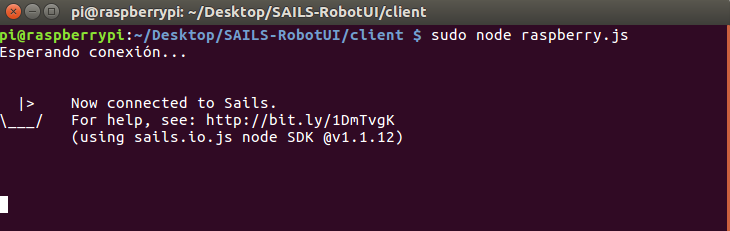
\includegraphics[scale=.6]{imagenes/manual-usuario/espera-conexion.png}
  \end{center}
  \caption{ Robot a la espera de conexión entrante.}
  \label{website:pagina-principal}
\end{figure}



% Este archivo es parte de la memoria del proyecto fin de carrera
% de Manuel López Urbina. Protegida bajo la licencia GFDL.
% Para más información, la licencia completa viene incluida en el
% fichero fdl-1.3.tex

% Copyright (C) 2017 Manuel López Urbina

\chapter{Comentarios finales}
\label{chap:conclusiones}

\section{Presupuesto}


\begin{table}[H]
  \begin{center}
    \begin{tabular}{|p{8cm}|p{2cm}|p{2cm}|p{2cm}|}
      \hline
      \vspace{+0.2in}{\textbf{Descripción}} & {\textbf{Unidades}} & {\textbf{Precio \EUR{} unidad }} & {\textbf{Total \EUR{}}}\\
      \hline
      \vspace{+0.2in}{Raspberry Pi 3 Modelo B} &  \vspace{+0.2in}{1} &  \vspace{+0.2in}{38,70} &  \vspace{+0.2in}{38,70}\\
      \hline
      \vspace{+0.2in}{Cámara USB alta definición} &  \vspace{+0.2in}{1} &  \vspace{+0.2in}{39,90} &  \vspace{+0.2in}{39,90}\\
      \hline
      \vspace{+0.2in}{Tarjeta de expansión con batería de Litio para Raspberry Pi} &  \vspace{+0.2in}{1} &  \vspace{+0.2in}{16,99} &  \vspace{+0.2in}{16,99}\\
      \hline
      \vspace{+0.2in}{Lipo batería (3.7v, 600mAh Lipo) } & \vspace{+0.2in}{1} & \vspace{+0.2in}{13,99} & \vspace{+0.2in}{13,99}\\
      \hline
      \vspace{+0.2in}{Indicador Tester de baterías Lipo} & \vspace{+0.2in}{1} & \vspace{+0.2in}{8,90} & \vspace{+0.2in}{8,90}\\
      \hline      
      \vspace{+0.2in}{Cargador baterías Lipo} & \vspace{+0.2in}{1} & \vspace{+0.2in}{21,90} & \vspace{+0.2in}{21,90}\\
      \hline
      \vspace{+0.2in}{Chasis vehículo Radiocontrol} & \vspace{+0.2in}{1} & \vspace{+0.2in}{54} & \vspace{+0.2in}{54}\\
      \hline
      \vspace{+0.2in}{Droplet DigitalOcean} & \vspace{+0.2in}{2 meses} & \vspace{+0.2in}{5/mes} & \vspace{+0.2in}{10}\\
      \hline        
      \vspace{+0.2in}{Horas de programación} & \vspace{+0.2in}{350 horas} & \vspace{+0.2in}{50/hora} & \vspace{+0.2in}{17500}\\
      \hline
    \end{tabular}
  \end{center}
\end{table}

\begin{table}[H]
  \begin{flushright}
    \begin{tabular}{p{8cm}p{2cm}}
      \vspace{+0.1in}\textbf{Total bruto:} &\vspace{+0.1in}{\EUR{17745,38}}\\
      \vspace{+0.1in}\textbf{I.V.A. \%: } & \vspace{+0.1in}{21\%}\\
      \vspace{+0.2in}\textbf{Total presupuesto:} & \vspace{+0.2in}{\EUR{21471,91}}\\
    \end{tabular}
  \end{flushright}
\end{table}


\section{Conclusiones}

La elaboración de este proyecto ha resultado muy gratificante a nivel personal. Uno de los motivos principales ha sido la necesidad de trabajar en numerosas áreas de conocimiento entre las que 
encontramos, por un lado la programación web, haciendo uso del framework Sails js, junto con el empleo de una base de datos no relacional. 
Todo ello combinado con la robótica. Algunas de las plataformas mencionadas eran desconocidas al inicio del desarrollo de proyecto y han sido adquiridas tras una amplia labor de investigación.\\

Entre los elementos desarrollados se destaca:

\begin{itemize}
 \item La elaboración de un vehículo de pruebas haciendo uso de una Raspberry Pi 3 Modelo B
 \item Aprendizaje a la utilización del framework Sails.js
 \item Aprendizaje al trabajo con eventos en tiempo real mediante el empleo de WebSockets, tecnología nunca utilizada por mí hasta la fecha
 \item Empleo de una base de datos no relacional como Mongo DB.
 \item Transmisión de gran cantidad de datos entre cliente servidor y servidor cliente. Streaming de vídeo y emisión de comandos entre otros datos.
\end{itemize}


Pienso que el resultado final del proyecto es ideal para aquellas personas aficionadas a la robótica y programación proporcionando una herramienta sea utilizable por la gran comunidad poseedora 
de cualquier proyecto robótico y que puedan compartirlo con el resto del mundo.\\

Una vez presentado podré continuar añadiendo mejoras y muchas cosas que tengo pensadas y que, posiblemente, se realicen para el proyecto del máster de Ingeniería de Sistemas y Computación que me 
encuentro realizando en la actualidad.

\section{Mejoras futuras}

La aplicación puede mejorarse en diversos aspectos. A continuación, se citan algunas de las mejoras que pueden llevarse a cabo:

\begin{itemize}

\item Incorporación de advertencias acústicas tras la detección de una señal de tráfico.

\item Mejora del diseño de la interfaz gráfica.

\item Permitir la definición de las teclas de control del teclado e incorporación de dispositivos tales como gamepads o joysticks.

\item Elaborar un generador de código para la exportación en los dispositivos robóticos, reduciendo por tanto las labores de programación.

\end{itemize}




%\backmatter % Apéndices, bibliografía ...

\backmatter


%\nocite{*}
\appendix
% Este archivo es parte de la memoria del proyecto fin de carrera
% de Manuel López Urbina. Protegida bajo la licencia GFDL.
% Para más información, la licencia completa viene incluida en el
% fichero fdl-1.3.tex

% Copyright (C) 2017 Manuel López Urbina

\newpage

\begin{appendix}
\backmatter

\chapter{Anexos}
\label{appendix:anexos}


Anexos con las instrucciones para la instalación de todos los componentes software empleados en el desarrollo del proyecto.\\

\section{Instalación de Node.js}


Instalación de los prerrequisitos:\\

\begin{lstlisting}[language=bash]
sudo apt-get install python-software-properties python g++ make
\end{lstlisting}


Si está utilizando Ubuntu 16.04, necesitará hacer los siguiente:\\

\begin{lstlisting}[language=bash]
sudo apt-get install software-properties-common
\end{lstlisting}


Añadimos el repositorio:\\

\begin{lstlisting}[language=bash]
sudo add-apt-repository ppa:chris-lea/node.js
\end{lstlisting}

Actualizamos la lista de paquetes:\\

\begin{lstlisting}[language=bash]
sudo apt-get update
\end{lstlisting}

Instalación de  Node.js:\\

\begin{lstlisting}[language=bash]
sudo apt-get install nodejs
\end{lstlisting}




\section{Instalación Sails.js}

Esta guía proporciona las pautas necesarias para la configuración de un entorno de trabajo para el desarrollo de aplicaciones Sails. Esta guía no cubre la instalación de en un entorno de producción.\\

\subsection{Prerrequisitos}

Partiendo de que se encuentra Node.js correctamente instalado en una máquina con Ubuntu 16.04.2 LTS. Ubuntu es una plataforma muy popular y utilizada en el desarrollo de Sails.js, al igual que otros sistemas operativos basados en Unix, como Mac OS X. La instalación es relativamente fácil y existe multitud de información gracias a su amplia comunidad de desarrolladores.\\

\begin{itemize}

\item{Una máquina con Ubuntu 16.04.2 LTS }
\item{Node js instalado.}


\end{itemize}

\subsection{Instalación}

A continuación detallaremos los pasos para la instalación de Sails. Lo primero que haremos es instalar Sails haciendo uso de npm, el gestor de paquetes que viene con el propio Node. Para ello, lo que vamos a hacer es ir directamente a la terminal y e introducir lo siguiente:\\

\begin{lstlisting}[language=bash]
sudo npm install sails -g
\end{lstlisting}

La opción -g, qe significa global, lo que hace es instalar Sails a nivel global, la cual nos permitirá acceder a las funcionalidades de Sails que emplearemos para la creación de nuestros proyectos.\\

Es posible que necesite permisos de administrador para instalar Sails a nivel global.\\

Para comprobar que la instalación se realizó correctamente, crearemos un proyecto inicial y levantaremos el servidor. Para ello introducimos en la terminal:\\

\begin{lstlisting}[language=bash]
sails new my_first_app
\end{lstlisting}

Cambiamos de directorio (cd) al nuevo directorio creado, en el cual nos aseguraremos de que Sails está correctamente instalado. Para ello arrancaremos el servidor y comprobaremos en nuestro navegador en localhost 1337 (localhost: 1337) que Sails está funcionando correctamente.\\


\begin{lstlisting}[language=bash]
cd my_fisrt_app
sails lift
\end{lstlisting}


Tras introducir en nuestro navegador \emph{localhost: 1337} debemos obtener el siguiente resultado:


\begin{figure}[H]
  \begin{center}
    \includegraphics[scale=0.3]{imagenes/running_sails.png}
  \end{center}
  \label{fig:logo}
 \caption{Iniciando Sails.}
\end{figure}


Y en nuestro navegador:\\

\begin{figure}[H]
  \begin{center}
    \includegraphics[scale=0.3]{imagenes/browser_sails.png}
  \end{center}
  \label{fig:logo}
 \caption{Sails en funcionamiento \protect\footnotemark.}
\end{figure}



\section{Instalación de MongoDB}

MongoDB es una base de datos libre y de código abierto NoSQL utilizada comúnmente en aplicaciones web modernas. Esta guía le ayudará a configurar MongoDB en su máquina para un entorno de aplicación de producción.\\

\subsection{Prerrequisitos}

Para seguir esta guía es necesario:
\begin{itemize}

\item{Una máquina con Ubuntu 14.04.}
\item{Un usuario con permisos de administrador (no root).}
\end{itemize}

\subsection{Instalación}


Para la instalación de MongoDB se puede optar con la versión disponible en los repositorios de paquetes de Ubuntu a pesar de que no sea la última versión disponible. Los repositorios propios de MongoDB proporcionan
la versión más actualizada siendo la forma recomendada de instalación. Para la instalación desde repositorios externos, Ubuntu garantiza la autenticidad de los paquetes de software al verificar que están firmados
con las claves GPG, por lo que primero tenemos que importar la clave para el repositorio oficial de MongoDB.\\

Para ello, debemos ejecutar:\\

\begin{lstlisting}[language=bash]
sudo apt-key adv --keyserver hkp://keyserver.ubuntu.com:80 --recv 7F0CEB10
\end{lstlisting}


Después de importar con éxito la clave, obtendremos el siguiente:\\

\begin{lstlisting}[language=bash]
Gpg: Número total procesado: 1
Gpg: importado: 1 (RSA: 1)
\end{lstlisting}

A continuación, tenemos que actualizar los detalles del repositorio de MongoDB para que APT sepa de dónde descargar los paquetes.\\

Introduzca el siguiente comando para crear un archivo de lista para MongoDB.\\

\begin{lstlisting}[language=bash]
echo "deb http://repo.mongodb.org/apt/ubuntu "\$(lsb_release -sc)"/mongodb-org/3.0 multiverse" | sudo tee /etc/apt/sources.list.d/mongodb-org-3.0.list
\end{lstlisting}

Después de agregar los detalles del repositorio, necesitamos actualizar la lista de paquetes.\\

\begin{lstlisting}[language=bash]
sudo apt-get update
\end{lstlisting}


Ahora podemos instalar el propio paquete MongoDB.\\

\begin{lstlisting}[language=bash]
sudo apt-get install -y mongodb-org
\end{lstlisting}

Este comando instalará varios paquetes que contengan la última versión estable de MongoDB junto con útiles herramientas de administración para el servidor MongoDB.\\

Después de la instalación del paquete, MongoDB se iniciará automáticamente. Puede comprobarlo ejecutando el siguiente comando.\\

\begin{lstlisting}[language=bash]
service mongodb status
\end{lstlisting}

Si MongoDB se está ejecutando, se mostrará una salida como la siguiente (con un ID de proceso diferente).\\

\begin{lstlisting}[language=bash]
 mongodb.service - An object/document-oriented database
   Loaded: loaded (/lib/systemd/system/mongodb.service; enabled; vendor preset: enabled)
   Active: active (running) since sáb 2017-02-04 13:07:01 CET; 11h ago
     Docs: man:mongod(1)
 Main PID: 807 (mongod)
    Tasks: 10
   Memory: 84.8M
      CPU: 4min 7.494s
   CGroup: /system.slice/mongodb.service
            - 807 /usr/bin/mongod --config /etc/mongodb.conf
\end{lstlisting}

También es posible detener, iniciar y reiniciar MongoDB utilizando los siguientes comandos:\\

\begin{lstlisting}[language=bash]
service mongodb stop
service mongodb start
\end{lstlisting}


\section{Instalación del control de versiones Git}

Para seguir esta guía es necesario disponer de una máquina con Ubuntu 14.04.\\

La forma más sencilla de tener Git instalado y configurado para su utilización es mediante el uso de los repositorios predeterminados de Ubuntu. 
Este es el método más rápido, pero, por contra puede ser que la versión disponible no sea la más reciente. 
Si necesita la última versión, deberá seguir los pasos para compilar Git desde el origen.\\

Si no necesitamos disponer de la última versión podemos instalarlo desde el repositorio de Ubuntu. Para ello introducimos los siguientes comandos en una terminal:\\

\begin{lstlisting}[language=bash]
sudo apt-get update
sudo apt-get install git
\end{lstlisting}

Esto descargará e instalará Git en el sistema. A continuación se describe los pasos para su configuración.

\subsection{Configuración}

Una vez que disponemos de Git instalado, necesitamos realizar una serie de pasos para añadir nuestros datos de acceso de nuestro repositorio.\\

La forma más sencilla de hacerlo es a través del comando \emph{git config} proporcionando nuestro nombre y dirección de correo electrónico. Esto es debido a que Git incorpora esta información en cada commit
que hacemos. Por ejemplo, si nuestro nombre es \emph{RobotUI} y nuestro email \emph{email@robotui.com}, los comandos de configuración serían los siguientes:\\

\begin{lstlisting}[language=bash]
 git config --global user.name "RobotUI"
 git config --global user.email "email@robotui.com"
\end{lstlisting}

Finalmente podemos comprobar todos los valores de configuración establecidos escribiendo:\\

\begin{lstlisting}[language=bash]
git config --list
\end{lstlisting}

Existen muchas más opciones configurables pero estos son los dos esenciales necesarios.\\

\section{Despliegue de una aplicación Sails}

Para el despliegue de la aplicación se a empleado una serie de herramientas y procedimientos que se encuentran recogidos en el recurso bibliográfico \cite{book:Deploying}, una referencia de gran 
utilidad para la puesta en producción de aquellas aplicaciones desarrolladas en cualquier framework Node.js. Caso del presente proyecto.\\

A continuación se describe una guía elemental, la cual ha sido seguida para la puesta en producción de RobotUI y que ha sido elaborada a partir de la citada referencia.\\

Primeramente, debemos definir el entorno de producción para nuestra aplicación Sails. Para ello editamos el fichero \emph{/config/env/production.js} introduciendo los siguientes datos:\\

\begin{itemize}
 \item Nombre de nuestra conexión de la base de datos la cual hemos definido en nuestro archivo \emph{config/connections.js}
 \item Dirección IP de nuestro servidor.
 \item Puerto por el que queremos correr nuestra aplicación.
\end{itemize}
  
Un ejemplo de configuración es el siguiente:

\begin{lstlisting}[language=JavaScript]
/**
 * Production environment settings
 *
 * This file can include shared settings for a production environment,
 * such as API keys or remote database passwords.  If you're using
 * a version control solution for your Sails app, this file will
 * be committed to your repository unless you add it to your .gitignore
 * file.  If your repository will be publicly viewable, don't add
 * any private information to this file!
 *
 */

module.exports = {

  /********************************************************************
   * Set the default database connection for models in the production *
   * environment (see config/connections.js and config/models.js )    *
   ********************************************************************/

  models: {
    connection: 'MongodbServer'
  },

  /********************************************************************
   * Set the port in the production environment to 80                 *
   ********************************************************************/

  port: 1337,

  /********************************************************************
   * Set the log level in production environment to "silent"          *
   ********************************************************************/

  log: {
    level: "silent"
  }

  proxyHost: '46.101.102.33',
  proxyPort: 1337

};
\end{lstlisting}

En el servidor de producción se ha utilizado Nginx \footnote{Nginx es un servidor web/proxy inverso ligero de alto rendimiento y un proxy para protocolos de correo electrónico (IMAP/POP3)} 
con la siguiente configuración:\\

\begin{lstlisting}[language=bash]

server {
  listen        80;
  server_name   46.101.102.33;


   listen 443 ssl;

   ssl_certificate /etc/nginx/ssl/nginx.crt;
   ssl_certificate_key /etc/nginx/ssl/nginx.key;

   location / {
        proxy_pass         http://46.101.102.33:1337/;

	proxy_http_version 1.1;
	proxy_set_header Upgrade $http_upgrade;
	proxy_set_header Connection "upgrade";
	proxy_set_header Host $host;

    }

}

\end{lstlisting}

Para arrancar la aplicación, se ha hecho uso del gestor de procesos Pm2, se introduce la siguiente orden: \\

\begin{lstlisting}[language=bash]
  sudo pm2 start app.js -x -- --prod
\end{lstlisting}


Para monitorizar la aplicación, Pm2 incorpora una herramienta de gestión de procesos. Para visualizarlo introducimos en una terminal:\\

\begin{lstlisting}[language=bash]
  sudo pm2 monit
\end{lstlisting}


Obteniendo un resultado similar al siguiente:

\begin{figure}[H]
  \begin{center}
    \includegraphics[scale=0.8]{imagenes/pm2-monit.jpg}\\
    \caption{Utilización del gestor de procesos Pm2 en el entorno de producción.}
  \end{center}
\end{figure}



\end{appendix}







\clearpage


\nocite{*}
\bibliography{robotui}{}
\bibliographystyle{plain}

\clearpage
\phantomsection  % so hyperref creates bookmarks

 \begin{center}

       Version 1.3, 3 November 2008


 Copyright \copyright{} 2000, 2001, 2002, 2007, 2008  Free Software Foundation, Inc.
 
 \bigskip
 
     \url{http://fsf.org/}
  
 \bigskip
 
 Everyone is permitted to copy and distribute verbatim copies
 of this license document, but changing it is not allowed.
\end{center}


\begin{center}
{\bf\large Preamble}
\end{center}

The purpose of this License is to make a manual, textbook, or other
functional and useful document ``free'' in the sense of freedom: to
assure everyone the effective freedom to copy and redistribute it,
with or without modifying it, either commercially or noncommercially.
Secondarily, this License preserves for the author and publisher a way
to get credit for their work, while not being considered responsible
for modifications made by others.

This License is a kind of ``copyleft'', which means that derivative
works of the document must themselves be free in the same sense.  It
complements the GNU General Public License, which is a copyleft
license designed for free software.

We have designed this License in order to use it for manuals for free
software, because free software needs free documentation: a free
program should come with manuals providing the same freedoms that the
software does.  But this License is not limited to software manuals;
it can be used for any textual work, regardless of subject matter or
whether it is published as a printed book.  We recommend this License
principally for works whose purpose is instruction or reference.


\begin{center}
{\Large\bf 1. APPLICABILITY AND DEFINITIONS\par}
\phantomsection
\addcontentsline{toc}{section}{1. APPLICABILITY AND DEFINITIONS}
\end{center}

This License applies to any manual or other work, in any medium, that
contains a notice placed by the copyright holder saying it can be
distributed under the terms of this License.  Such a notice grants a
world-wide, royalty-free license, unlimited in duration, to use that
work under the conditions stated herein.  The ``\textbf{Document}'', below,
refers to any such manual or work.  Any member of the public is a
licensee, and is addressed as ``\textbf{you}''.  You accept the license if you
copy, modify or distribute the work in a way requiring permission
under copyright law.

A ``\textbf{Modified Version}'' of the Document means any work containing the
Document or a portion of it, either copied verbatim, or with
modifications and/or translated into another language.

A ``\textbf{Secondary Section}'' is a named appendix or a front-matter section of
the Document that deals exclusively with the relationship of the
publishers or authors of the Document to the Document's overall subject
(or to related matters) and contains nothing that could fall directly
within that overall subject.  (Thus, if the Document is in part a
textbook of mathematics, a Secondary Section may not explain any
mathematics.)  The relationship could be a matter of historical
connection with the subject or with related matters, or of legal,
commercial, philosophical, ethical or political position regarding
them.

The ``\textbf{Invariant Sections}'' are certain Secondary Sections whose titles
are designated, as being those of Invariant Sections, in the notice
that says that the Document is released under this License.  If a
section does not fit the above definition of Secondary then it is not
allowed to be designated as Invariant.  The Document may contain zero
Invariant Sections.  If the Document does not identify any Invariant
Sections then there are none.

The ``\textbf{Cover Texts}'' are certain short passages of text that are listed,
as Front-Cover Texts or Back-Cover Texts, in the notice that says that
the Document is released under this License.  A Front-Cover Text may
be at most 5 words, and a Back-Cover Text may be at most 25 words.

A ``\textbf{Transparent}'' copy of the Document means a machine-readable copy,
represented in a format whose specification is available to the
general public, that is suitable for revising the document
straightforwardly with generic text editors or (for images composed of
pixels) generic paint programs or (for drawings) some widely available
drawing editor, and that is suitable for input to text formatters or
for automatic translation to a variety of formats suitable for input
to text formatters.  A copy made in an otherwise Transparent file
format whose markup, or absence of markup, has been arranged to thwart
or discourage subsequent modification by readers is not Transparent.
An image format is not Transparent if used for any substantial amount
of text.  A copy that is not ``Transparent'' is called ``\textbf{Opaque}''.

Examples of suitable formats for Transparent copies include plain
ASCII without markup, Texinfo input format, LaTeX input format, SGML
or XML using a publicly available DTD, and standard-conforming simple
HTML, PostScript or PDF designed for human modification.  Examples of
transparent image formats include PNG, XCF and JPG.  Opaque formats
include proprietary formats that can be read and edited only by
proprietary word processors, SGML or XML for which the DTD and/or
processing tools are not generally available, and the
machine-generated HTML, PostScript or PDF produced by some word
processors for output purposes only.

The ``\textbf{Title Page}'' means, for a printed book, the title page itself,
plus such following pages as are needed to hold, legibly, the material
this License requires to appear in the title page.  For works in
formats which do not have any title page as such, ``Title Page'' means
the text near the most prominent appearance of the work's title,
preceding the beginning of the body of the text.

The ``\textbf{publisher}'' means any person or entity that distributes
copies of the Document to the public.

A section ``\textbf{Entitled XYZ}'' means a named subunit of the Document whose
title either is precisely XYZ or contains XYZ in parentheses following
text that translates XYZ in another language.  (Here XYZ stands for a
specific section name mentioned below, such as ``\textbf{Acknowledgements}'',
``\textbf{Dedications}'', ``\textbf{Endorsements}'', or ``\textbf{History}''.)  
To ``\textbf{Preserve the Title}''
of such a section when you modify the Document means that it remains a
section ``Entitled XYZ'' according to this definition.

The Document may include Warranty Disclaimers next to the notice which
states that this License applies to the Document.  These Warranty
Disclaimers are considered to be included by reference in this
License, but only as regards disclaiming warranties: any other
implication that these Warranty Disclaimers may have is void and has
no effect on the meaning of this License.


\begin{center}
{\Large\bf 2. VERBATIM COPYING\par}
\phantomsection
\addcontentsline{toc}{section}{2. VERBATIM COPYING}
\end{center}

You may copy and distribute the Document in any medium, either
commercially or noncommercially, provided that this License, the
copyright notices, and the license notice saying this License applies
to the Document are reproduced in all copies, and that you add no other
conditions whatsoever to those of this License.  You may not use
technical measures to obstruct or control the reading or further
copying of the copies you make or distribute.  However, you may accept
compensation in exchange for copies.  If you distribute a large enough
number of copies you must also follow the conditions in section~3.

You may also lend copies, under the same conditions stated above, and
you may publicly display copies.


\begin{center}
{\Large\bf 3. COPYING IN QUANTITY\par}
\phantomsection
\addcontentsline{toc}{section}{3. COPYING IN QUANTITY}
\end{center}


If you publish printed copies (or copies in media that commonly have
printed covers) of the Document, numbering more than 100, and the
Document's license notice requires Cover Texts, you must enclose the
copies in covers that carry, clearly and legibly, all these Cover
Texts: Front-Cover Texts on the front cover, and Back-Cover Texts on
the back cover.  Both covers must also clearly and legibly identify
you as the publisher of these copies.  The front cover must present
the full title with all words of the title equally prominent and
visible.  You may add other material on the covers in addition.
Copying with changes limited to the covers, as long as they preserve
the title of the Document and satisfy these conditions, can be treated
as verbatim copying in other respects.

If the required texts for either cover are too voluminous to fit
legibly, you should put the first ones listed (as many as fit
reasonably) on the actual cover, and continue the rest onto adjacent
pages.

If you publish or distribute Opaque copies of the Document numbering
more than 100, you must either include a machine-readable Transparent
copy along with each Opaque copy, or state in or with each Opaque copy
a computer-network location from which the general network-using
public has access to download using public-standard network protocols
a complete Transparent copy of the Document, free of added material.
If you use the latter option, you must take reasonably prudent steps,
when you begin distribution of Opaque copies in quantity, to ensure
that this Transparent copy will remain thus accessible at the stated
location until at least one year after the last time you distribute an
Opaque copy (directly or through your agents or retailers) of that
edition to the public.

It is requested, but not required, that you contact the authors of the
Document well before redistributing any large number of copies, to give
them a chance to provide you with an updated version of the Document.


\begin{center}
{\Large\bf 4. MODIFICATIONS\par}
\phantomsection
\addcontentsline{toc}{section}{4. MODIFICATIONS}
\end{center}

You may copy and distribute a Modified Version of the Document under
the conditions of sections 2 and 3 above, provided that you release
the Modified Version under precisely this License, with the Modified
Version filling the role of the Document, thus licensing distribution
and modification of the Modified Version to whoever possesses a copy
of it.  In addition, you must do these things in the Modified Version:

\begin{itemize}
\item[A.] 
   Use in the Title Page (and on the covers, if any) a title distinct
   from that of the Document, and from those of previous versions
   (which should, if there were any, be listed in the History section
   of the Document).  You may use the same title as a previous version
   if the original publisher of that version gives permission.
   
\item[B.]
   List on the Title Page, as authors, one or more persons or entities
   responsible for authorship of the modifications in the Modified
   Version, together with at least five of the principal authors of the
   Document (all of its principal authors, if it has fewer than five),
   unless they release you from this requirement.
   
\item[C.]
   State on the Title page the name of the publisher of the
   Modified Version, as the publisher.
   
\item[D.]
   Preserve all the copyright notices of the Document.
   
\item[E.]
   Add an appropriate copyright notice for your modifications
   adjacent to the other copyright notices.
   
\item[F.]
   Include, immediately after the copyright notices, a license notice
   giving the public permission to use the Modified Version under the
   terms of this License, in the form shown in the Addendum below.
   
\item[G.]
   Preserve in that license notice the full lists of Invariant Sections
   and required Cover Texts given in the Document's license notice.
   
\item[H.]
   Include an unaltered copy of this License.
   
\item[I.]
   Preserve the section Entitled ``History'', Preserve its Title, and add
   to it an item stating at least the title, year, new authors, and
   publisher of the Modified Version as given on the Title Page.  If
   there is no section Entitled ``History'' in the Document, create one
   stating the title, year, authors, and publisher of the Document as
   given on its Title Page, then add an item describing the Modified
   Version as stated in the previous sentence.
   
\item[J.]
   Preserve the network location, if any, given in the Document for
   public access to a Transparent copy of the Document, and likewise
   the network locations given in the Document for previous versions
   it was based on.  These may be placed in the ``History'' section.
   You may omit a network location for a work that was published at
   least four years before the Document itself, or if the original
   publisher of the version it refers to gives permission.
   
\item[K.]
   For any section Entitled ``Acknowledgements'' or ``Dedications'',
   Preserve the Title of the section, and preserve in the section all
   the substance and tone of each of the contributor acknowledgements
   and/or dedications given therein.
   
\item[L.]
   Preserve all the Invariant Sections of the Document,
   unaltered in their text and in their titles.  Section numbers
   or the equivalent are not considered part of the section titles.
   
\item[M.]
   Delete any section Entitled ``Endorsements''.  Such a section
   may not be included in the Modified Version.
   
\item[N.]
   Do not retitle any existing section to be Entitled ``Endorsements''
   or to conflict in title with any Invariant Section.
   
\item[O.]
   Preserve any Warranty Disclaimers.
\end{itemize}

If the Modified Version includes new front-matter sections or
appendices that qualify as Secondary Sections and contain no material
copied from the Document, you may at your option designate some or all
of these sections as invariant.  To do this, add their titles to the
list of Invariant Sections in the Modified Version's license notice.
These titles must be distinct from any other section titles.

You may add a section Entitled ``Endorsements'', provided it contains
nothing but endorsements of your Modified Version by various
parties---for example, statements of peer review or that the text has
been approved by an organization as the authoritative definition of a
standard.

You may add a passage of up to five words as a Front-Cover Text, and a
passage of up to 25 words as a Back-Cover Text, to the end of the list
of Cover Texts in the Modified Version.  Only one passage of
Front-Cover Text and one of Back-Cover Text may be added by (or
through arrangements made by) any one entity.  If the Document already
includes a cover text for the same cover, previously added by you or
by arrangement made by the same entity you are acting on behalf of,
you may not add another; but you may replace the old one, on explicit
permission from the previous publisher that added the old one.

The author(s) and publisher(s) of the Document do not by this License
give permission to use their names for publicity for or to assert or
imply endorsement of any Modified Version.


\begin{center}
{\Large\bf 5. COMBINING DOCUMENTS\par}
\phantomsection
\addcontentsline{toc}{section}{5. COMBINING DOCUMENTS}
\end{center}


You may combine the Document with other documents released under this
License, under the terms defined in section~4 above for modified
versions, provided that you include in the combination all of the
Invariant Sections of all of the original documents, unmodified, and
list them all as Invariant Sections of your combined work in its
license notice, and that you preserve all their Warranty Disclaimers.

The combined work need only contain one copy of this License, and
multiple identical Invariant Sections may be replaced with a single
copy.  If there are multiple Invariant Sections with the same name but
different contents, make the title of each such section unique by
adding at the end of it, in parentheses, the name of the original
author or publisher of that section if known, or else a unique number.
Make the same adjustment to the section titles in the list of
Invariant Sections in the license notice of the combined work.

In the combination, you must combine any sections Entitled ``History''
in the various original documents, forming one section Entitled
``History''; likewise combine any sections Entitled ``Acknowledgements'',
and any sections Entitled ``Dedications''.  You must delete all sections
Entitled ``Endorsements''.

\begin{center}
{\Large\bf 6. COLLECTIONS OF DOCUMENTS\par}
\phantomsection
\addcontentsline{toc}{section}{6. COLLECTIONS OF DOCUMENTS}
\end{center}

You may make a collection consisting of the Document and other documents
released under this License, and replace the individual copies of this
License in the various documents with a single copy that is included in
the collection, provided that you follow the rules of this License for
verbatim copying of each of the documents in all other respects.

You may extract a single document from such a collection, and distribute
it individually under this License, provided you insert a copy of this
License into the extracted document, and follow this License in all
other respects regarding verbatim copying of that document.


\begin{center}
{\Large\bf 7. AGGREGATION WITH INDEPENDENT WORKS\par}
\phantomsection
\addcontentsline{toc}{section}{7. AGGREGATION WITH INDEPENDENT WORKS}
\end{center}


A compilation of the Document or its derivatives with other separate
and independent documents or works, in or on a volume of a storage or
distribution medium, is called an ``aggregate'' if the copyright
resulting from the compilation is not used to limit the legal rights
of the compilation's users beyond what the individual works permit.
When the Document is included in an aggregate, this License does not
apply to the other works in the aggregate which are not themselves
derivative works of the Document.

If the Cover Text requirement of section~3 is applicable to these
copies of the Document, then if the Document is less than one half of
the entire aggregate, the Document's Cover Texts may be placed on
covers that bracket the Document within the aggregate, or the
electronic equivalent of covers if the Document is in electronic form.
Otherwise they must appear on printed covers that bracket the whole
aggregate.


\begin{center}
{\Large\bf 8. TRANSLATION\par}
\phantomsection
\addcontentsline{toc}{section}{8. TRANSLATION}
\end{center}


Translation is considered a kind of modification, so you may
distribute translations of the Document under the terms of section~4.
Replacing Invariant Sections with translations requires special
permission from their copyright holders, but you may include
translations of some or all Invariant Sections in addition to the
original versions of these Invariant Sections.  You may include a
translation of this License, and all the license notices in the
Document, and any Warranty Disclaimers, provided that you also include
the original English version of this License and the original versions
of those notices and disclaimers.  In case of a disagreement between
the translation and the original version of this License or a notice
or disclaimer, the original version will prevail.

If a section in the Document is Entitled ``Acknowledgements'',
``Dedications'', or ``History'', the requirement (section~4) to Preserve
its Title (section~1) will typically require changing the actual
title.


\begin{center}
{\Large\bf 9. TERMINATION\par}
\phantomsection
\addcontentsline{toc}{section}{9. TERMINATION}
\end{center}


You may not copy, modify, sublicense, or distribute the Document
except as expressly provided under this License.  Any attempt
otherwise to copy, modify, sublicense, or distribute it is void, and
will automatically terminate your rights under this License.

However, if you cease all violation of this License, then your license
from a particular copyright holder is reinstated (a) provisionally,
unless and until the copyright holder explicitly and finally
terminates your license, and (b) permanently, if the copyright holder
fails to notify you of the violation by some reasonable means prior to
60 days after the cessation.

Moreover, your license from a particular copyright holder is
reinstated permanently if the copyright holder notifies you of the
violation by some reasonable means, this is the first time you have
received notice of violation of this License (for any work) from that
copyright holder, and you cure the violation prior to 30 days after
your receipt of the notice.

Termination of your rights under this section does not terminate the
licenses of parties who have received copies or rights from you under
this License.  If your rights have been terminated and not permanently
reinstated, receipt of a copy of some or all of the same material does
not give you any rights to use it.


\begin{center}
{\Large\bf 10. FUTURE REVISIONS OF THIS LICENSE\par}
\phantomsection
\addcontentsline{toc}{section}{10. FUTURE REVISIONS OF THIS LICENSE}
\end{center}


The Free Software Foundation may publish new, revised versions
of the GNU Free Documentation License from time to time.  Such new
versions will be similar in spirit to the present version, but may
differ in detail to address new problems or concerns.  See
http://www.gnu.org/copyleft/.

Each version of the License is given a distinguishing version number.
If the Document specifies that a particular numbered version of this
License ``or any later version'' applies to it, you have the option of
following the terms and conditions either of that specified version or
of any later version that has been published (not as a draft) by the
Free Software Foundation.  If the Document does not specify a version
number of this License, you may choose any version ever published (not
as a draft) by the Free Software Foundation.  If the Document
specifies that a proxy can decide which future versions of this
License can be used, that proxy's public statement of acceptance of a
version permanently authorizes you to choose that version for the
Document.


\begin{center}
{\Large\bf 11. RELICENSING\par}
\phantomsection
\addcontentsline{toc}{section}{11. RELICENSING}
\end{center}


``Massive Multiauthor Collaboration Site'' (or ``MMC Site'') means any
World Wide Web server that publishes copyrightable works and also
provides prominent facilities for anybody to edit those works.  A
public wiki that anybody can edit is an example of such a server.  A
``Massive Multiauthor Collaboration'' (or ``MMC'') contained in the
site means any set of copyrightable works thus published on the MMC
site.

``CC-BY-SA'' means the Creative Commons Attribution-Share Alike 3.0
license published by Creative Commons Corporation, a not-for-profit
corporation with a principal place of business in San Francisco,
California, as well as future copyleft versions of that license
published by that same organization.

``Incorporate'' means to publish or republish a Document, in whole or
in part, as part of another Document.

An MMC is ``eligible for relicensing'' if it is licensed under this
License, and if all works that were first published under this License
somewhere other than this MMC, and subsequently incorporated in whole
or in part into the MMC, (1) had no cover texts or invariant sections,
and (2) were thus incorporated prior to November 1, 2008.

The operator of an MMC Site may republish an MMC contained in the site
under CC-BY-SA on the same site at any time before August 1, 2009,
provided the MMC is eligible for relicensing.


\begin{center}
{\Large\bf ADDENDUM: How to use this License for your documents\par}
\phantomsection
\addcontentsline{toc}{section}{ADDENDUM: How to use this License for your documents}
\end{center}

To use this License in a document you have written, include a copy of
the License in the document and put the following copyright and
license notices just after the title page:

\bigskip
\begin{quote}
    Copyright \copyright{}  YEAR  YOUR NAME.
    Permission is granted to copy, distribute and/or modify this document
    under the terms of the GNU Free Documentation License, Version 1.3
    or any later version published by the Free Software Foundation;
    with no Invariant Sections, no Front-Cover Texts, and no Back-Cover Texts.
    A copy of the license is included in the section entitled ``GNU
    Free Documentation License''.
\end{quote}
\bigskip
    
If you have Invariant Sections, Front-Cover Texts and Back-Cover Texts,
replace the ``with \dots\ Texts.'' line with this:

\bigskip
\begin{quote}
    with the Invariant Sections being LIST THEIR TITLES, with the
    Front-Cover Texts being LIST, and with the Back-Cover Texts being LIST.
\end{quote}
\bigskip
    
If you have Invariant Sections without Cover Texts, or some other
combination of the three, merge those two alternatives to suit the
situation.

If your document contains nontrivial examples of program code, we
recommend releasing these examples in parallel under your choice of
free software license, such as the GNU General Public License,
to permit their use in free software.

%---------------------------------------------------------------------


\end{document}

